\documentclass[fleqn,usenatbib]{mnras}
%
%\hypersetup{draft}  %%% only for draft

%\usepackage{natbib}
\usepackage{xr-hyper}

%from mnras:
\usepackage{hyperref}	% Hyperlinks
\hypersetup{colorlinks=true,linkcolor=blue,citecolor=blue,filecolor=blue,urlcolor=blue}

\usepackage[russian]{babel}
\usepackage[utf8]{inputenc}

\usepackage{mathptmx}
\usepackage[T1]{fontenc}
\usepackage{ae,aecompl}
\usepackage{graphicx}	% Including figure files
\usepackage{amsmath}	% Advanced maths commands
\usepackage{amssymb}	% Extra maths symbols
\usepackage{multicol}   % Multi-column entries in tables
\usepackage{bm}         % Bold maths symbols, including upright Greek
\usepackage{pdflscape}  % Landscape pages
\usepackage{enumitem}
\usepackage{xspace}
\usepackage{hhline}
\def\beq#1{\begin{equation}\label{#1}}
\def\eeq{\end{equation}}

\usepackage{comment}

% for referecnes in tables
\usepackage{array}
\usepackage{etoolbox}
\usepackage{multirow}

\usepackage{color}
\newcommand{\red}[1]{\textcolor{red}{#1}}
\newcommand{\blue}[1]{\textcolor{blue}{#1}}
\newcommand{\green}[1]{\textcolor{green}{#1}}
\newcommand{\achtung}[1]{\textcolor{red}{//#1//}}

% for newpage
\usepackage{titlesec}
\newcommand{\sectionbreak}{\newpage}
\newcommand{\subsectionbreak}{\newpage}

\title[ShortTitle]{Title}
\author[Borisov et al.]{Victor Borisov, Alexander Meshcheryakov %\newauthor 
}
\date{September 2020}

%%%%%%%%%%%%%%%%%%%%
%DO NOT CHANGE
\makeatletter
\newcommand*{\addFileDependency}[1]{% argument=file name and extension
  \typeout{(#1)}
  \@addtofilelist{#1}
  \IfFileExists{#1}{}{\typeout{No file #1.}}
}
\makeatother

\newcommand*{\myexternaldocument}[1]{%
    \externaldocument{#1}%
    \addFileDependency{#1.tex}%
    \addFileDependency{#1.aux}%
}
%%%%%%%%%%%%%%%%%%%%
%CHANGE
%\myexternaldocument{pdf_figures}
%%%%%%%%%%%%%%%%%%%

\usepackage{pdflscape}
\begin{document}

% for references in tables
\newcounter{rowcntr}[table]
\renewcommand{\therowcntr}{\arabic{rowcntr}}
% A new columntype to apply automatic stepping
\newcolumntype{N}{>{\refstepcounter{rowcntr}\therowcntr}c}
% Reset the rowcntr counter at each new tabular
\AtBeginEnvironment{tabular}{\setcounter{rowcntr}{0}}

\newcommand{\expnumber}[2]{{#1}\mathrm{e}{#2}}

\maketitle
\begin{abstract}
Проведено исследование, построение и сравнение моделей вероятностных прогнозов фотометрических красных смещений (photo-z) на основе алгоритма случайного леса  с использованием данных современных астрономических обзоров SDSS, PanStarrs и DESI Legacy Survey для построения трехмерной карты квазаров.

Предложена модель photo-z, значительно превосходящая (в ~2 раза) по точности (метрики точечных прогнозов — нормализованное медианное абсолютное отклонение NMAD и доля выбросов n>0.15) лучшие модели (SOTA) известные в литературе. Для рентгеновских источников в тестовой области неба Stripe82X получена точность NMAD = 0.034 / 0.064 / 0.067 и n>0.15 = 0.079 / 0.170 / 0.163 для предложенной модели / шаблонной модели Ananna, 2017 / нейросетевой модели Brescia, 2019, соответственно.
\end{abstract}

% ===============================================================================
% ===============================================================================
% ===============================================================================


\section{Inctoduction}

On July 13, 2019 the SRG X-ray observatory
was launched from the Baikonur cosmodrome. On Dec. 8th, 2019 SRG started its first All-Sky Survey, which will consist of 8 repeated six month long scans of the entire sky. eROSITA telescope \citep{2020arXiv201003477P} onboard SRG operates in the soft X-ray band (0.3–8\,keV) and will detect $\sim3$ millions X-ray AGNs at the end of survey. In order to construct a large-scale structure map of X-ray Universe with eROSITA, accurate measurements of cosmological redshifts for extragalactic X-ray sources (mostly quasars) are needed.

Redshift measurement methods \citep{2019NatAs...3..212S} can be divided into spectroscopic (spec-z, $z_{sp}$) and photometric (photo-z, $\hat{z}_{ph}$). Spec-z's are time consuming task for faint optical objects ($r\gtrsim22^{mag}$). On the other hand, photo-z measurements can be based on data from modern large photometric sky surveys, it is much cheaper in observational resources than spec-z but also less accurate. 

В задаче измерения photo-z возникает проблема мультимодальности прогнозов. На рисунке (тут нужен хороший рисунок с примерами двух спектров и прогнозами) представлен пример спектров двух галактик, находящихся на разном красном смещении. Видно, что в некотором диапазоне излучения их спектры сильно похожи, и, как следствие, сильно похожи фотометрические признаки (отмечены черными точками на графике). Таким образом получается неоднозначное соответствие прогнозов признакам, и точечная оценка, построенная на основе этих признаков, скорее всего, будет неверной. Поэтому необходимо прогнозировать не само значение красного смещения объекта, а распределение значения красного смещения объекта. Такой прогноз называется вероятностным фотометрическим красным смещением (вероятностный photo-z). Вероятностный photo-z позволит вычислять доверительные интервалы, оценивать надежность прогнозов.

In this work we present machine learning models for X-ray sources probabilistic photo-z predictions, based on photometric data from 4 modern sky surveys (SDSS, Pan-STARRS1, DESI Legacy Imaging Survey, and WISE).

\subsection{Related works}
Общие подходы к решению задачи прогноза photo-z описываются в \cite{bib:nature_photoz}. Все решения, предлагаемые для решения данной задачи можно разделить на 2 группы: основанные на использовании физических моделей (Physically motivated methods, шаблонные модели) и основанные на использовании данных (Data driven methods), т.е. с применением технологий машинного обучения.

Суть методов на основе шаблонов состоит в использовании спектров типовых объектов различных классов. На основе спектра строится шаблон -- физическая модель предсказывающая значение фотометрических признаков по значению красного смещения, составляется библиотека шаблонов. Далее производится поиск оптимального шаблона, на котором достигается минимальная ошибка между предсказанными фотометрическими признаками и измеренными, путем минимизации критерия \(\mathcal{X}^2\)
\begin{equation}
    \mathcal{X}^2 (z, T, A) = \sum_i^{N_{filters}} (\frac{F_{obs}^i - A~F_{pred}^i(T, z)}{\sigma_{obs}^i})^2,
\end{equation}
где \(z\) -- значение красного смещения, \(N_{filetrs}\) -- количество фильтров (фотометрических признаков), \(F_{obs}^i\) и \(\sigma_{obs}^i\) -- наблюдаемое значение \(i\)-ого признака и ошибка на него, \(F_{pred}^i(T, z)\) -- значение \(i\)-ого признака, полученное из шаблона \(T\) для красного смещения \(z\), \(A\) -- фактор нормализации. Таким образом определяется не только красное смещение объекта, но и его тип.

Такие модели представлены в пакетах ...

Однако, такие методы показывают точность хуже методов машинного обучения при наличии большой репрезентативной обучающей выборки. Основные алгоритмы, применяемые для прогнозов фотометрических красных смещений -- искусственные нейронные сети, ближайшие соседи и методы на основе ансамблей деревьев решений, которые показывают лучшую точность в данной задаче.

В пакете ANNz2 \cite{bib:annz2} реализованы методы на основе многослойного персептрона, деревьев бустинга (boosted decision trees) и регрессии k-ближайших соседей. Реализованные в пакете алгоритмы позволяют оценивать достоверность прогноза, и в качестве финального прогноза дается лучший из прогнозов ансамбля моделей или взвешенная сумма прогнозов. В сравнении использовался ансамбль из пяти многослойных персептронов с архитектурой слоёв 6:12:12:1, где на вход подавались данные шести фильтров ugrizy и на выходном слое получается прогноз photo-z. Каждый персептрон обучался со случайной инициализацией параметров.

В пакете CMNN \cite{bib:cmnn} для прогноза photo-z используется метод ближайших соседей. В качестве признаков выступают, так называемые цвета (отношение яркостей между разными фильтрами), расстоянием между соседями выступает расстояние Махалонобиса
\begin{equation}
    D_M = \sum_j^{N_{colors}} \frac{(c_{j,train} - c_{j,test})^2}{(\delta c_{j,test})^2},
\end{equation}
и в качестве прогноза дается взвешенная сумма целевых признаков соседей с весами, обратными расстояниям до них.
%\achtung{пока не очень въехал в описание. Дописать}

FlexZBoost \cite{bib:flexzboost} представляет собой набор общих методов адаптации алгоритмов оценки условного среднего для оценки условной плотности распределения целевого признака. Для этого неизвестная функция плотности раскладывается по ортонормированному базису. В статье было использовано преобразование Фурье. Далее коэффициенты Фурье вычисляются как точечная оценка с использованием выбранного алгоритма машинного обучения (в статье использовался xgboost).

Алгоритм GPz \cite{bib:gpz} основан на использовании гауссовых процессов. 

METAPhoR \cite{bib:metaphor} представляет собой алгоритм вероятностных прогнозов photo-z, позволяющий адаптировать алгоритмы регрессии для получения вероятностных оценок. По умолчанию используется многослойный персептрон обучение которого происходит квазиньютоновским алгоритмом (Multi Layer Perceptron with Quasi Newton Algorithm, MLPQNA) минимизацией ошибки MSE с применением L2-регуляризации. Для получения вероятностного прогноза признаки объекта разыгрываются в соответствии с ошибками измерений на них. Модели, реализованные в данном пакете были применены в статье Brescia для прогноза photo-z рентгеновских источников.

В пакете SkyNet \cite{bib:skynet} используются многослойный персептрон, обучаемый методом градиентного спуска второго порядка минимизацией кросс-энтропийной функции потерь, то есть решается задача классификации. Область определения целевого признака разбивается на 200 интервалов, объект принадлежит к некоторому классу, если его целевой признак принадлежит к соответствующему интервалу. Вероятностный прогноз получается из двухсот выходов выходного слоя с функцией активации softmax нейронной сети, на вход алгоритма подаются измерения и ошибки измерения шести фотометрических признаков (всего 12 входов).

В TPZ \cite{bib:tpz} используется алгоритм случайного леса без ограничения глубины. Вероятностный прогноз получается путем решения множества задач бинарной классификации: область определения целевого признака разбивается на интервалы, и для каждого интервала строится модель классификации, которая определяет, принадлежит ли значение целевого признака заданному интервалу или не принадлежит. Вероятностный прогноз представляет собой набор вероятностей принадлежности значения целевого признака тому или иному интервалу.

В \cite{bib:mesch} были предложены методы, основанные на использовании случайного леса и квантильного градиентного бустинга, для получения вероятностных прогнозов фотометрических красных смещений.

Метод, основанный на алгоритме случайного леса, заключается в получении прогноза распределения в виде независимой выборки точечных прогнозов деревьев, построенных без ограничения глубины. Независимость достигается за счет того, что деревья в методе случайного леса строятся независимо на случайных подвыборках обучающей выборки. Далее для оценки непрерывной функции плотности вероятности (для получения вероятностного прогноза) используется ядерная оценка плотности.

Метод квантильного градиентного бустинга заключается в обучении модели с квантильной функцией потерь, которую для фиксированного значения \(\alpha \in [0,1]\) можно записать следующим образом
\begin{equation}
    l(y_i, \hat{y}_{\alpha, i}) = (1-\alpha)|y_i - \hat{y}_{\alpha, i}|\mathbb{I}[y \leq \hat{y}_{\alpha, i}] + \alpha|y_i - \hat{y}_{\alpha, i}|\mathbb{I}[y > \hat{y}_{\alpha, i}],
\end{equation}
где \(y_i\) - истинное значение, \(\hat{y}_{\alpha, i}\) - предсказанное значений целевой переменной. Таким образом, вероятностный прогноз, являющийся результатом работы этого алгоритма будет представлен ансамблем заданных квантилей. Стоит заметить, что в методе градиентного бустинга каждое следующее дерево строится для антиградиента предыдущего, что делает их не независимыми, и делает невозможным получение вероятностного прогноза в представлении выборки независимых значений, как это реализовано в случайном лесе.

% ===============================================================================
% ===============================================================================
% ===============================================================================

\section{Data}
\subsection{Photometric data}
We use photometric data from SDSS DR14 \citep{2018ApJS..235...42A}, Pan-STARRS1 DR2 \citep{2018AAS...23110201C}, DESI LIS DR8 \citep{2019AJ....157..168D} sky surveys and WISE forced photometry \citep{2010AJ....140.1868W}. A brief description of each of the sky surveys is given in Table \ref{tab:catalogs_comparison}.

It is important to note that only Pan-STARRS covers the entire eastern hemisphere of the sky, so photo-z models based only on Pan-STARRS data are of particular interest to the Russian eRosita consortium.

\begin{table*}
    \caption{Comparison of photometric sky surveys from which photometric data were used by the presence of filters and the coverage area of the sky.}
    \label{tab:catalogs_comparison}
    \centering
    \begin{tabular}{|l|c|c|c|}
    \hline
        Survey & Filters & Types of fluxes & Sky coverage (square degrees) \\
    \hline
        SDSS DR16 & u,g,r,i,z,w1,w2 & PSF, cModel & 14555 (1/3 of the sky) \\
        Pan-STARRS1 DR2 & g,r,i,z,y & PSF, Kron & 30000 (3/4 of the sky) \\
        DESI LIS & g,r,z,w1,w2,w3,w4 & Model & 14000 (1/3 of the sky) \\[1ex]
        \hline
    \end{tabular}
\end{table*}

\subsection{Spectral Data}


\subsection{Features Set}
To build Photo-z models, we construct an expert set of features. To do this, we first calculate hyperbolic magnitudes from fluxes:
\begin{equation}\label{eq:asinhmag}
    mag = \Bigg[asinh\Bigg(\frac{f/f_0}{2 \times b/f_0}\Bigg) + \log(b/f_0)\Bigg] \times \Bigg(\frac{-2.5}{\log 10}\Bigg) ~,
\end{equation}
where $f~[nanomaggies]$ и $b = \sigma_{flux}~[nanomaggies]$ - value and error of flux, and (\url{https://www.legacysurvey.org/dr9/description/#photometry})
\begin{equation}
    f_0 = 1~[nanomaggie] = 10^{-(48.6+22.5)/2.5}~[erg/cm^2/Hz].
\end{equation}
Magnitudes values makes it possible to use information about objects with negative fluxes. In addition, the values calculated by this formula contain information about flux errors. It is important to outline, that in SDSS survey $b$ is a mean error for a sky section, while we take the object's flux error $b = \sigma_{flux}~[nanomaggies]$.

Описать свойства гиперболического синуса.

However, we will give all charts in more standard AB-values, which are calculated by the following formula: the formula is taken from here: \url{https://www.sdss.org/dr12/algorithms/magnitudes/} (звезда яркосьтю 1 nanomaggie имеет величину 22.5 \url{https://www.sdss.org/dr12/help/glossary/#mag_pogson})
\begin{equation}\label{eq:mag_ab}
    m_{AB} = [22.5 mag] - 2.5 \log_{10} \frac{f}{f_0}
\end{equation}

Table \ref{tab:featuressets} below provides a description of the feature sets. Different models use photometry from different surveys, so the feature set is determined primarily by the source of the photometric data and spitted into magnitudes and colors. Then, if the model uses DESI LIS model magnitudes, we exclude the attributes associated with these magnitudes from the other surveys. That is why each of SDSS and Pan-STARRS features sets are splitted into two (\ref{feats:sdss-mags-1} and \ref{feats:sdss-mags-2}, \ref{feats:sdss-colors-1} and \ref{feats:sdss-colors-2} for SDSS; \ref{feats:ps-mags-1} and \ref{feats:ps-mags-2}, \ref{feats:ps-colors-1} and \ref{feats:ps-colors-2} for Pan-STARRS). For example, if the model uses the r and g mags from DESI LIS, the model r and g mags from the SDSS survey will not be included in the model, nor will the r-g color based on the SDSS model values. However, because of the absence of PSF magnitudes in DESI LIS, colors like $r_{psf} - r_{cmodel}$ and $r_{psf} - g_{psf}$ based on SDSS magnitudes will be included. Similarly for the Kron magnitudes of the Pan-STARRS surveys.

Models are presented in Table \ref{tab:models}. In total, we present 5 models: model \ref{model:pw} based on Pan-STARRS and WISE photometry, model \ref{model:pdw} based on Pan-STARRS, DESI LIS and WISE photometry, model \ref{model:dw} based on DESI LIS and WISE photometry, model \ref{model:psw} based on SDSS, Pan-STARRS and WISE photometry and model \ref{model:spdw} based on photometry from all four sources.

We use 2 sources of WISE photometry: DESI LIS survey and forced photometry for Pan-STARRS1 survey (Burenin et.al., 202X). The second must be used primarily for model \ref{model:pw}, since using WISE from DESI LIS, which has much less coverage than Pan-STARRS, the goal of building this model -- a forecast over the entire Russian eRosita sky -- will not be achieved.

\begin{table*}
    \label{tab:featuressets}
    \caption{Description of the sets of features used. The first column contains the name of the feature set, the second column contains the feature set number, and the third column lists the magnitudes in the format $passband_{survey, type}$ (for DESI LIS magnitudes -- $passband_{LS}$) and colors based on those magnitudes in the format $mag_1 - mag_2$ that are part of the feature sets. Magnitudes are calculated by the hyperbolic sine formula \eqref{eq:asinhmag}. <<LS>> stands for <<DESI LIS>> and <<PS>> stands for Pan-STARRS1.}
    \newcounter{FeatsSetNumber}[figure] 
    \renewcommand{\theFeatsSetNumber}{\arabic{FeatsSetNumber}}
    \setcounter{FeatsSetNumber}{0}
	\begin{tabular}{ r l p{10cm} }
	\hline
	    Features sets & No. & Features \\
    \hline
        \multirow{2}{*}{SDSS mags} & \refstepcounter{FeatsSetNumber}\theFeatsSetNumber\label{feats:sdss-mags-1} & \(u_{SDSS,psf}\), \(g_{SDSS,psf}\), \(r_{SDSS,psf}\), \(i_{SDSS,psf}\), \(z_{SDSS,psf}\), \(u_{SDSS,cmodel}\), \(i_{SDSS,cmodel}\), \\
         & \refstepcounter{FeatsSetNumber}\theFeatsSetNumber\label{feats:sdss-mags-2} & \(g_{SDSS,cmodel}\), \(r_{SDSS,cmodel}\), \(z_{SDSS,cmodel}\), \\
        \multirow{2}{*}{SDSS colors} & \refstepcounter{FeatsSetNumber}\theFeatsSetNumber\label{feats:sdss-colors-1} & \(u_{SDSS,psf}-g_{SDSS,psf}\), \(u_{SDSS,psf}-r_{SDSS,psf}\), \(u_{SDSS,psf}-i_{SDSS,psf}\), \(u_{SDSS,psf}-z_{SDSS,psf}\), \(u_{SDSS,psf}-u_{SDSS,cmodel}\), \(g_{SDSS,psf}-i_{SDSS,psf}\), \(g_{SDSS,psf}-g_{SDSS,cmodel}\), \(r_{SDSS,psf}-i_{SDSS,psf}\), \(i_{SDSS,psf}-z_{SDSS,psf}\), \(i_{SDSS,psf}-i_{SDSS,cmodel}\), \\
         & \refstepcounter{FeatsSetNumber}\theFeatsSetNumber\label{feats:sdss-colors-2} & \(g_{SDSS,psf}-r_{SDSS,psf}\), \(g_{SDSS,psf}-z_{SDSS,psf}\), \(r_{SDSS,psf}-z_{SDSS,psf}\), \(r_{SDSS,psf}-r_{SDSS,cmodel}\), \(z_{SDSS,psf}-z_{SDSS,cmodel}\) \\
    \hline
        \multirow{2}{*}{Pan-STARRS mags} & \refstepcounter{FeatsSetNumber}\theFeatsSetNumber\label{feats:ps-mags-1} & \(g_{PS,psf}\), \(r_{PS,psf}\), \(i_{PS,psf}\), \(z_{PS,psf}\), \(y_{PS,psf}\), \(i_{PS,kron}\), \(y_{PS,kron}\) \\
         & \refstepcounter{FeatsSetNumber}\theFeatsSetNumber\label{feats:ps-mags-2} & \(g_{PS,kron}\), \(r_{PS,kron}\), \(z_{PS,kron}\) \\
        \multirow{2}{*}{Pan-STARRS colors} & \refstepcounter{FeatsSetNumber}\theFeatsSetNumber\label{feats:ps-colors-1} & \(g_{PS,psf}-i_{PS,psf}\), \(g_{PS,psf}-y_{PS,psf}\), \(r_{PS,psf}-i_{PS,psf}\), \(r_{PS,psf}-y_{PS,psf}\), \(i_{PS,psf}-z_{PS,psf}\), \(i_{PS,psf}-y_{PS,psf}\), \(z_{PS,psf}-y_{PS,psf}\), \(i_{PS,psf}-i_{PS,kron}\), \(y_{PS,psf}-y_{PS,kron}\) \\
         & \refstepcounter{FeatsSetNumber}\theFeatsSetNumber\label{feats:ps-colors-2} & \(g_{PS,psf}-r_{PS,psf}\) \(g_{PS,psf}-z_{PS,psf}\), \(r_{PS,psf}-z_{PS,psf}\), \(g_{PS,psf}-g_{PS,kron}\), \(r_{PS,psf}-r_{PS,kron}\), \(z_{PS,psf}-z_{PS,kron}\) \\
    \hline
        DESI LIS mags & \refstepcounter{FeatsSetNumber}\theFeatsSetNumber\label{feats:ls-mags-1} & \(g_{LS}\), \(r_{LS}\), \(z_{LS}\) \\
        DESI LIS colors & \refstepcounter{FeatsSetNumber}\theFeatsSetNumber\label{feats:ls-colors-1} & \(g_{LS}-r_{LS}\), \(g_{LS}-z_{LS}\), \(r_{LS}-z_{LS}\) \\
    \hline
        WISE mags & \refstepcounter{FeatsSetNumber}\theFeatsSetNumber\label{feats:wise-mags-1} & \(w1\), \(w2\) \\
        WISE colors & \refstepcounter{FeatsSetNumber}\theFeatsSetNumber\label{feats:wise-colors-1} & \(w1-w2\) \\
    \hline
        SDSS + DESI LIS colors & \refstepcounter{FeatsSetNumber}\theFeatsSetNumber\label{feats:sdss-ls-colors-1} & \(g_{SDSS,cmodel}-g_{LS}\), \(r_{SDSS,cmodel}-r_{LS}\), \(z_{SDSS,cmodel}-z_{LS}\) \\
        SDSS + WISE colors & \refstepcounter{FeatsSetNumber}\theFeatsSetNumber\label{feats:sdss-wise-colors-1} & \(u_{SDSS,cmodel}-w1\), \(u_{SDSS,cmodel}-w2\), \(g_{SDSS,cmodel}-w1\), \(g_{SDSS,cmodel}-w2\), \(r_{SDSS,cmodel}-w1\), \(r_{SDSS,cmodel}-w2\), \(i_{SDSS,cmodel}-w1\), \(i_{SDSS,cmodel}-w2\), \(z_{SDSS,cmodel}-w1\), \(z_{SDSS,cmodel}-w2\) \\
        Pan-STARRS + DESI LIS colors & \refstepcounter{FeatsSetNumber}\theFeatsSetNumber\label{feats:ps-ls-colors-1} & \(g_{PS,kron}-g_{LS}\), \(r_{PS,kron}-r_{LS}\), \(z_{PS,kron}-z_{LS}\) \\
        Pan-STARRS + WISE colors & \refstepcounter{FeatsSetNumber}\theFeatsSetNumber\label{feats:ps-wise-colors-1} & \(g_{PS,kron}-w1\), \(g_{PS,kron}-w2\), \(r_{PS,kron}-w1\), \(r_{PS,kron}-w2\), \(i_{PS,kron}-w1\), \(i_{PS,kron}-w2\), \(z_{PS,kron}-w1\), \(z_{PS,kron}-w2\), \(y_{PS,kron}-w1\), \(y_{PS,kron}-w2\) \\
        DESI LIS + WISE colors & \refstepcounter{FeatsSetNumber}\theFeatsSetNumber\label{feats:ls-wise-colors-1} & \(g_{LS}-w1\), \(g_{LS}-w2\), \(r_{LS}-w1\), \(r_{LS}-w2\), \(z_{LS}-w1\), \(z_{LS}-w2\) \\
    \hline
    \end{tabular}
\end{table*}

\begin{table*}
    \caption{Models description. The first column indicates the model number, the next four columns indicate the photometry sources used by the model (SDSS, Pan-STARRS, DESI LIS, and WISE, respectively). For SDSS, PS, and LS <<+>> means use of survey photometry, skip -- non-use. For WISE, <<LS>> means use of infrared data from DESI LIS, <<RB>> -- forced photometry for the Pan-STARRS survey from the paper (Burenin et.al., 202X). The last column lists the feature sets from Table \ref{tab:featuressets} used to build the models. <<LS>> stands for <<DESI LIS>> and <<PS>> stands for Pan-STARRS1.}
    \label{tab:models}
    \centering
    \newcounter{ModelNumber}[figure] 
    \renewcommand{\theModelNumber}{\arabic{ModelNumber}}
    \setcounter{ModelNumber}{0}
    \begin{tabular}{r c c c c l}
    \hline
        {}                      & \multicolumn{4}{c}{Data} & {}\\
        No. & SDSS & PS & LS & WISE & Feature sets used \\
    \hline
        \refstepcounter{ModelNumber}\theModelNumber\label{model:pw} & & + & & RB & \ref{feats:ps-mags-1}, \ref{feats:ps-mags-2}, \ref{feats:ps-colors-1}, \ref{feats:ps-colors-2}, \ref{feats:wise-mags-1}, \ref{feats:wise-colors-1}, \ref{feats:ps-wise-colors-1} \\ %Pan-STARRS mags (1 and 2) and colors (1 and 2), WISE mags and colors, Pan-STARRS + WISE colors \\
        \refstepcounter{ModelNumber}\theModelNumber\label{model:pdw} & & + & + & LS & \ref{feats:ps-mags-1}, \ref{feats:ps-colors-1}, \ref{feats:ls-mags-1}, \ref{feats:ls-colors-1}, \ref{feats:wise-mags-1}, \ref{feats:wise-colors-1}, \ref{feats:ps-ls-colors-1}, \ref{feats:ps-wise-colors-1} \\ % Pan-STARRS mags (1) and colors (1), DESI LIS mags and colors, WISE mags and colors, Pan-STARRS + DESI LIS colors, Pan-STARRS + WISE colors \\
        \refstepcounter{ModelNumber}\theModelNumber\label{model:dw} & & & + & LS & \ref{feats:ls-mags-1}, \ref{feats:ls-colors-1}, \ref{feats:wise-mags-1}, \ref{feats:wise-colors-1}, \ref{feats:ls-wise-colors-1} \\ % DESI LIS mags and colors, WISE mags and colors, DESI LIS + WISE colors \\
        \refstepcounter{ModelNumber}\theModelNumber\label{model:spw} & + & + & & RB & \ref{feats:sdss-mags-1}, \ref{feats:sdss-mags-2}, \ref{feats:ps-colors-1}, \ref{feats:ps-colors-2}, \ref{feats:wise-mags-1}, \ref{feats:wise-colors-1}, \ref{feats:sdss-wise-colors-1}, \ref{feats:ps-wise-colors-1} \\
        \refstepcounter{ModelNumber}\theModelNumber\label{model:spdw} & + & + & + & LS & \ref{feats:sdss-mags-1}, \ref{feats:sdss-colors-1}, \ref{feats:ps-mags-1}, \ref{feats:ps-colors-1}, \ref{feats:ls-mags-1}, \ref{feats:ls-colors-1}, \ref{feats:wise-mags-1}, \ref{feats:wise-colors-1}, \ref{feats:sdss-wise-colors-1}, \ref{feats:sdss-ls-colors-1}, \ref{feats:ps-wise-colors-1} \\ % SDSS mags and colors, Pan-STARRS mags (1) and colors (1), DESI LIS mags and colors, WISE mags and colors, SDSS + WISE colors, SDSS + DESI LIS colors, Pan-STARRS + WISE colors \\
    \hline
    \end{tabular}
\end{table*}


\subsection{Account for extinction}

To account for Galactic extinction, the $E(B-V)$ estimates from the DESI LIS catalog and the $A/E(B-V)$ coefficients from \citep{2011ApJ...737..103S}. The adjusted values of fluxes and errors on fluxes are calculated using the following formulas:
\begin{equation}
    flux_{ebv, pb} = flux_{pb} 10^{0.4 * dm_{pb}},
\end{equation}
\begin{equation}
    \sigma_{flux_{ebv, pb}} = \sigma_{flux_{pb}} 10^{0.4 * dm_{pb}},
\end{equation}
where $dm_{pb} = E(B-V) * [A/E(B-V)]_{pb}$, $[A/E(B-V)]_{pb}$ is coefficient from \citep{2011ApJ...737..103S} for $pb$ filter, $flux_{ebv, pb}$ и $\sigma_{flux_{ebv, pb}}$ are flux and errors on flux in $pb$ filter.

\subsection{Train sample}

The SDSS spectral catalog was used to compile a large training sample (see Table \ref{tab:samples}). Optical galaxies SDSS DR14 and quasars SDSS DR14q Paris'18 were balanced by class in order to approximate the distribution of X-ray sources. The distribution of the training sample objects was then aligned as shown in Figure 1. and the VHzQs quasars (Ross \& Corss, 20??) were added. The properties of the sample are shown in more detail in Figures \ref{fig:data_distribution} and \ref{fig:data-dist-mags-ab}.

\begin{figure*}
    \centering
    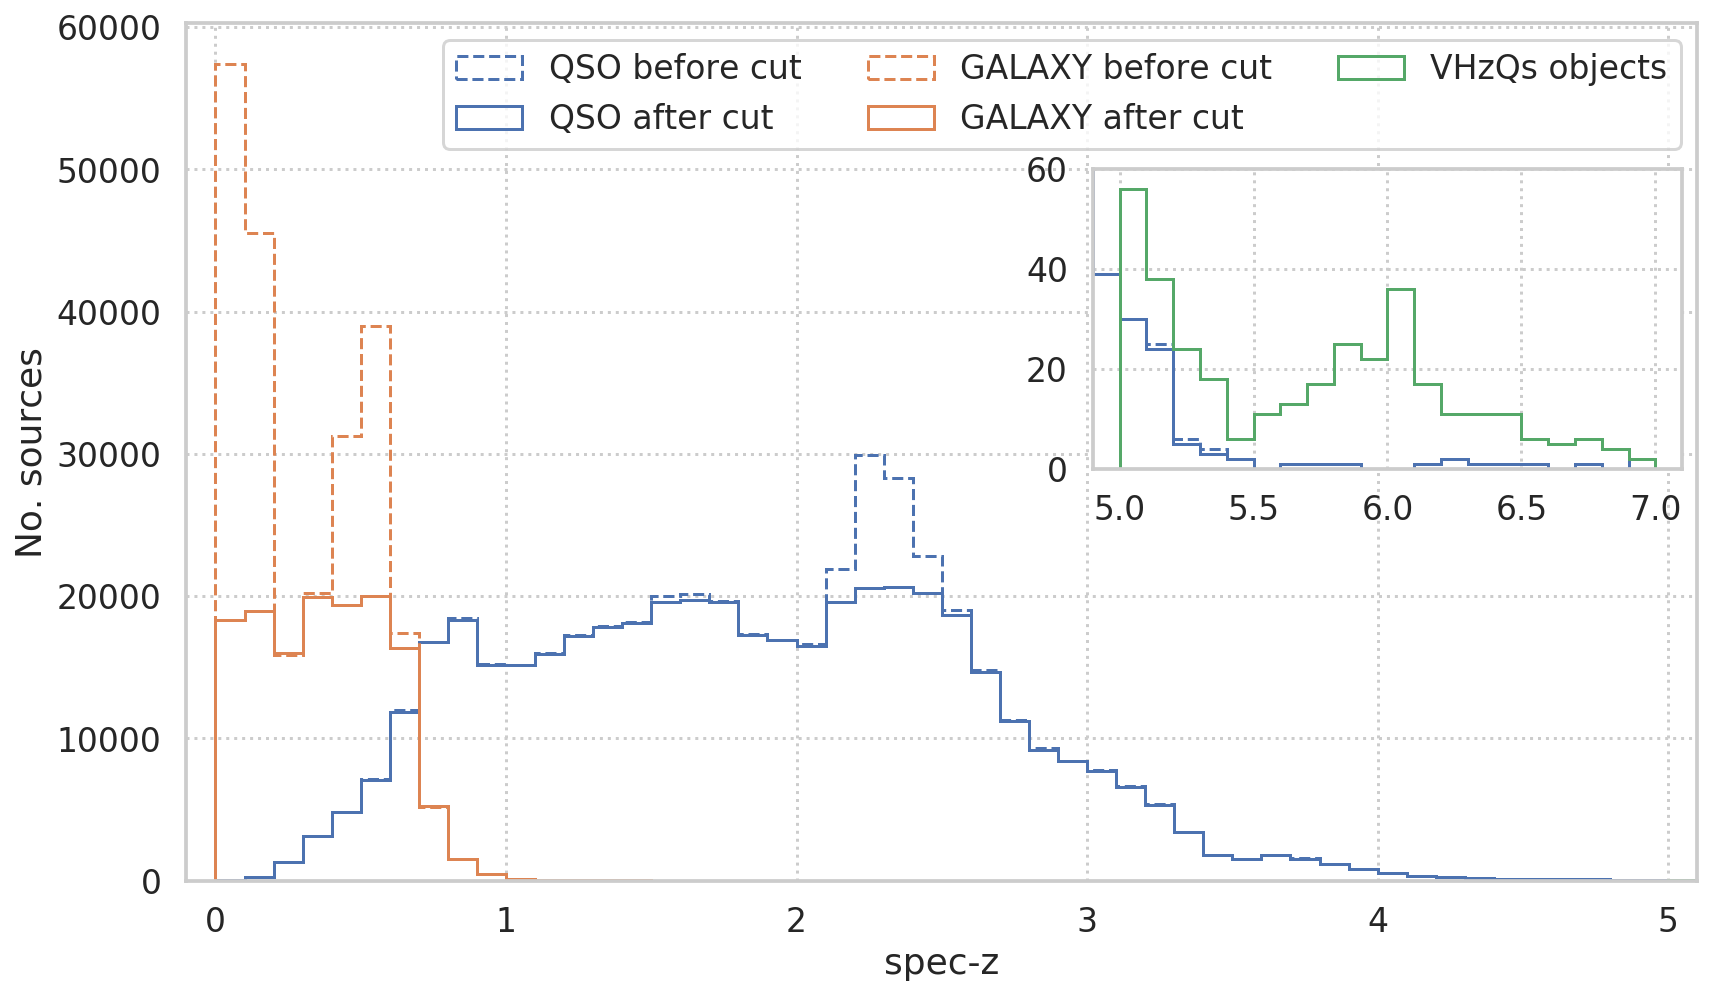
\includegraphics[width=0.95\linewidth]{images/train-peaks-cut.png}
    \caption{Pre-processing of the training sample. The histogram of the distribution of the SDSS DR14 galaxies included in the sample is shown in orange, the SDSS DR14q quasars are shown in blue, and the VHzQs quasars are shown in green. The dashed lines are the distributions before the alignment, and the solid lines are the distributions after the alignment.}
    \label{fig:train-peaks-cut}
\end{figure*}

\subsection{Stripe82X test sample}
The Stripe82X sample of X-ray objects was first presented in (Ananna, 2017). This sample is currently the largest sample of X-ray objects with a qualitative classification by spectra, and it is marked by hand, which makes it the main test sample for the comparison of photo-z X-ray object models. The results chapter will compare our models with State-Of-The-Art models: the template model (Ananna, 2017) and the neural network model (Brescia, 2019). The properties of the sample are shown in more detail in Figures \ref{fig:data_distribution} and \ref{fig:data-dist-mags-ab}.

\subsection{Test sample of DR16q objects}
For a more detailed analysis of the behavior of the models on objects with $spec-z > 3$, a test sample of quasars was compiled. The objects with the most reliably measured spectral redshifts (\texttt{Z\_CONF == 3 and SOURCEZ == VI}) were selected from the SDSS DR16q spectral catalog, and the distribution peak at $z \sim 3$ was cut off, similarly to the training sample. The properties of the sample are shown in more detail in Figures \ref{fig:data_distribution} and \ref{fig:data-dist-mags-ab}.

\begin{table*}
	\begin{tabular}{rlllllll}
            \hline
            {} & \multicolumn{3}{l}{No. sources} & \multicolumn{4}{l}{With photometry from} \\
            Sample &       Total &  Galaxy &     QSO &             DESI LIS & Pan-STARRS &    SDSS & All 3 surveys \\
            \hline
            Train                                                          &      586176 &  136428 &  449748 &               580511 &     578815 &  578650 &        577049 \\
            Stripe82X                                                      &        2909 &     648 &    1771 &                 2898 &       2434 &    2862 &          2407 \\
            Stripe82X ($\expnumber{3}{-15} <= FSoft < \expnumber{1}{-14}$) &        1160 &     297 &     656 &                 1155 &        942 &    1137 &           929 \\
            Stripe82X ($\expnumber{1}{-14} <= FSoft < \expnumber{4}{-14}$) &        1263 &     194 &     859 &                 1260 &       1082 &    1248 &          1073 \\
            Stripe82X ($FSoft > \expnumber{4}{-14}$)                       &         242 &      17 &     186 &                  240 &        211 &     238 &           209 \\
            DR16q w/o train                                                &       38091 &       0 &   38091 &                37949 &      32520 &   37877 &         32466 \\
            \hline
            \end{tabular}
            \label{tab:samples}
            \caption{Description of the samples used. The first column gives the name of the sample, the next three columns are the number of objects (total, separate galaxies, separate quasars), the next four columns are the number of objects with full DESI LIS photometry, Pan-STARRS, SDSS and all three surveys simultaneously, respectively.}
\end{table*}

\begin{figure*}
    \centering
    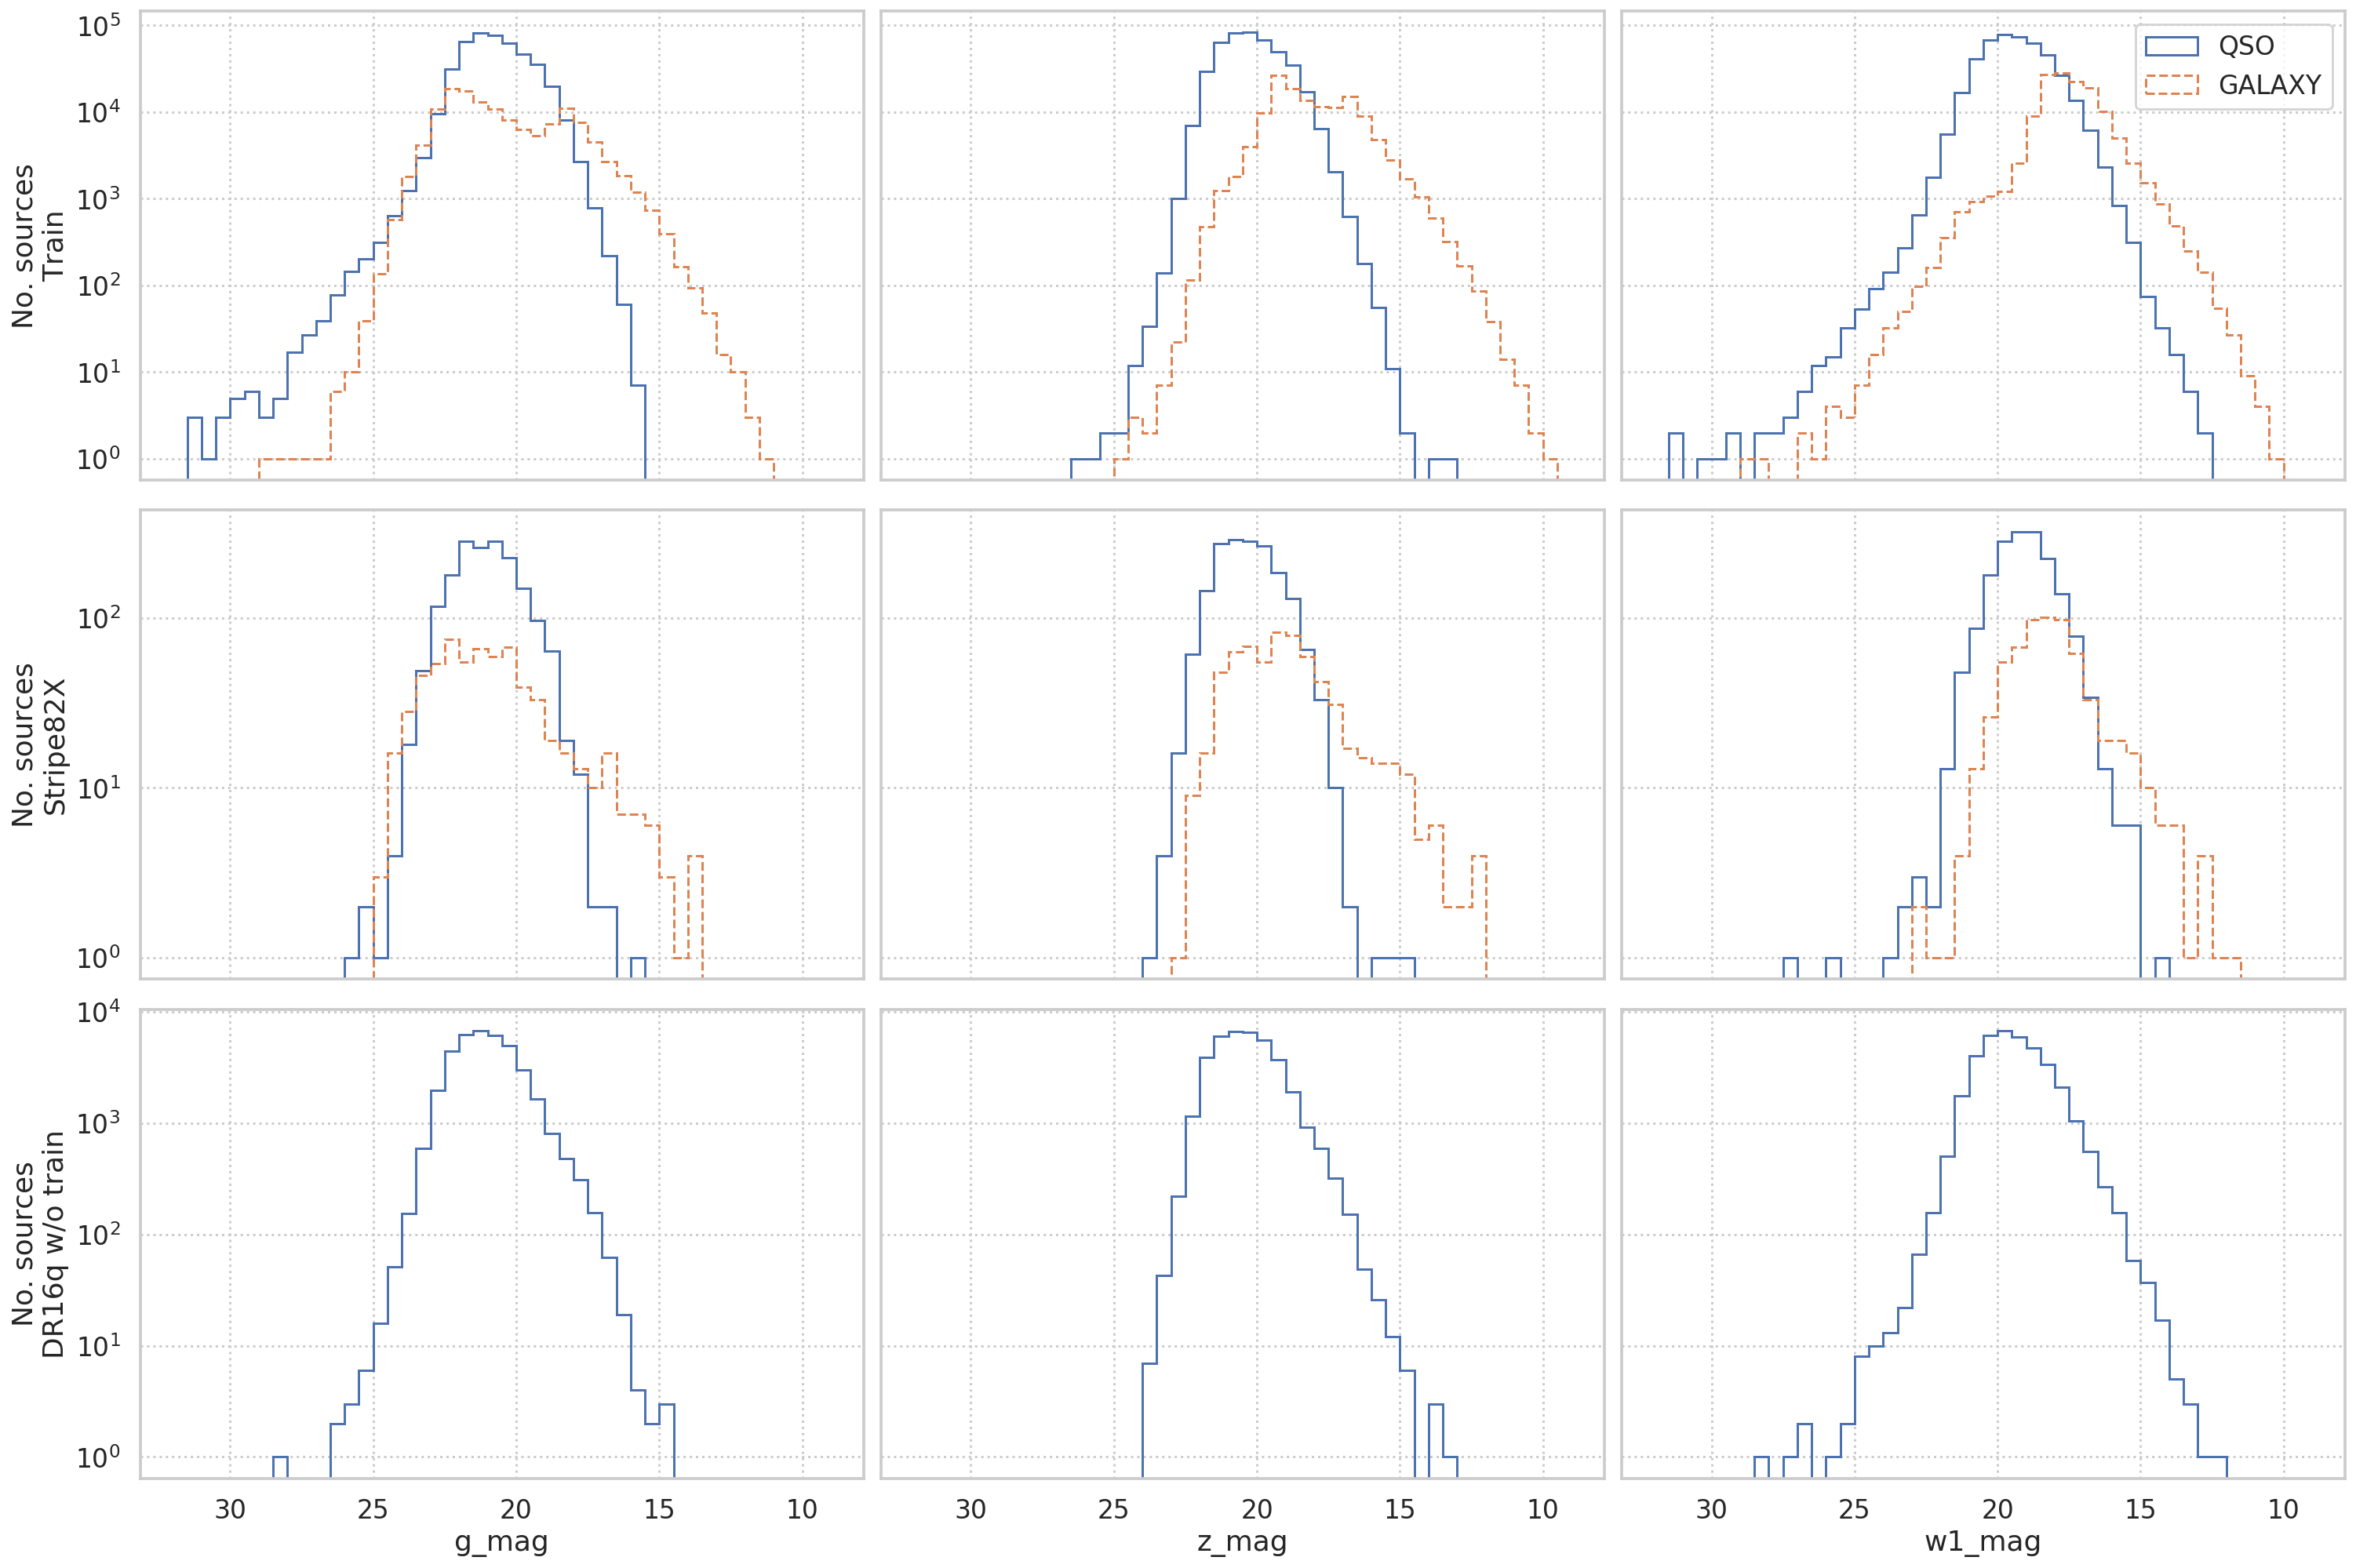
\includegraphics[width=0.9\linewidth]{images/data-dist-mags-ab.png}
    \caption{Histograms of object distributions in the samples according to the magnitude value of \eqref{eq:mag_ab} in the blue (g), red (z), and infrared (w1) filters. The first line of the graphs is the distribution of the training sample, the second line of the graphs is the distribution of the Stripe82X sample, and the third line is the distribution of the test sample of the SDSS DR16q quasars. The blue solid line shows the distribution of quasars, and the orange line shows the distribution of galaxies.}
    \label{fig:data-dist-mags-ab}
\end{figure*}

\begin{figure*}
    \centering
    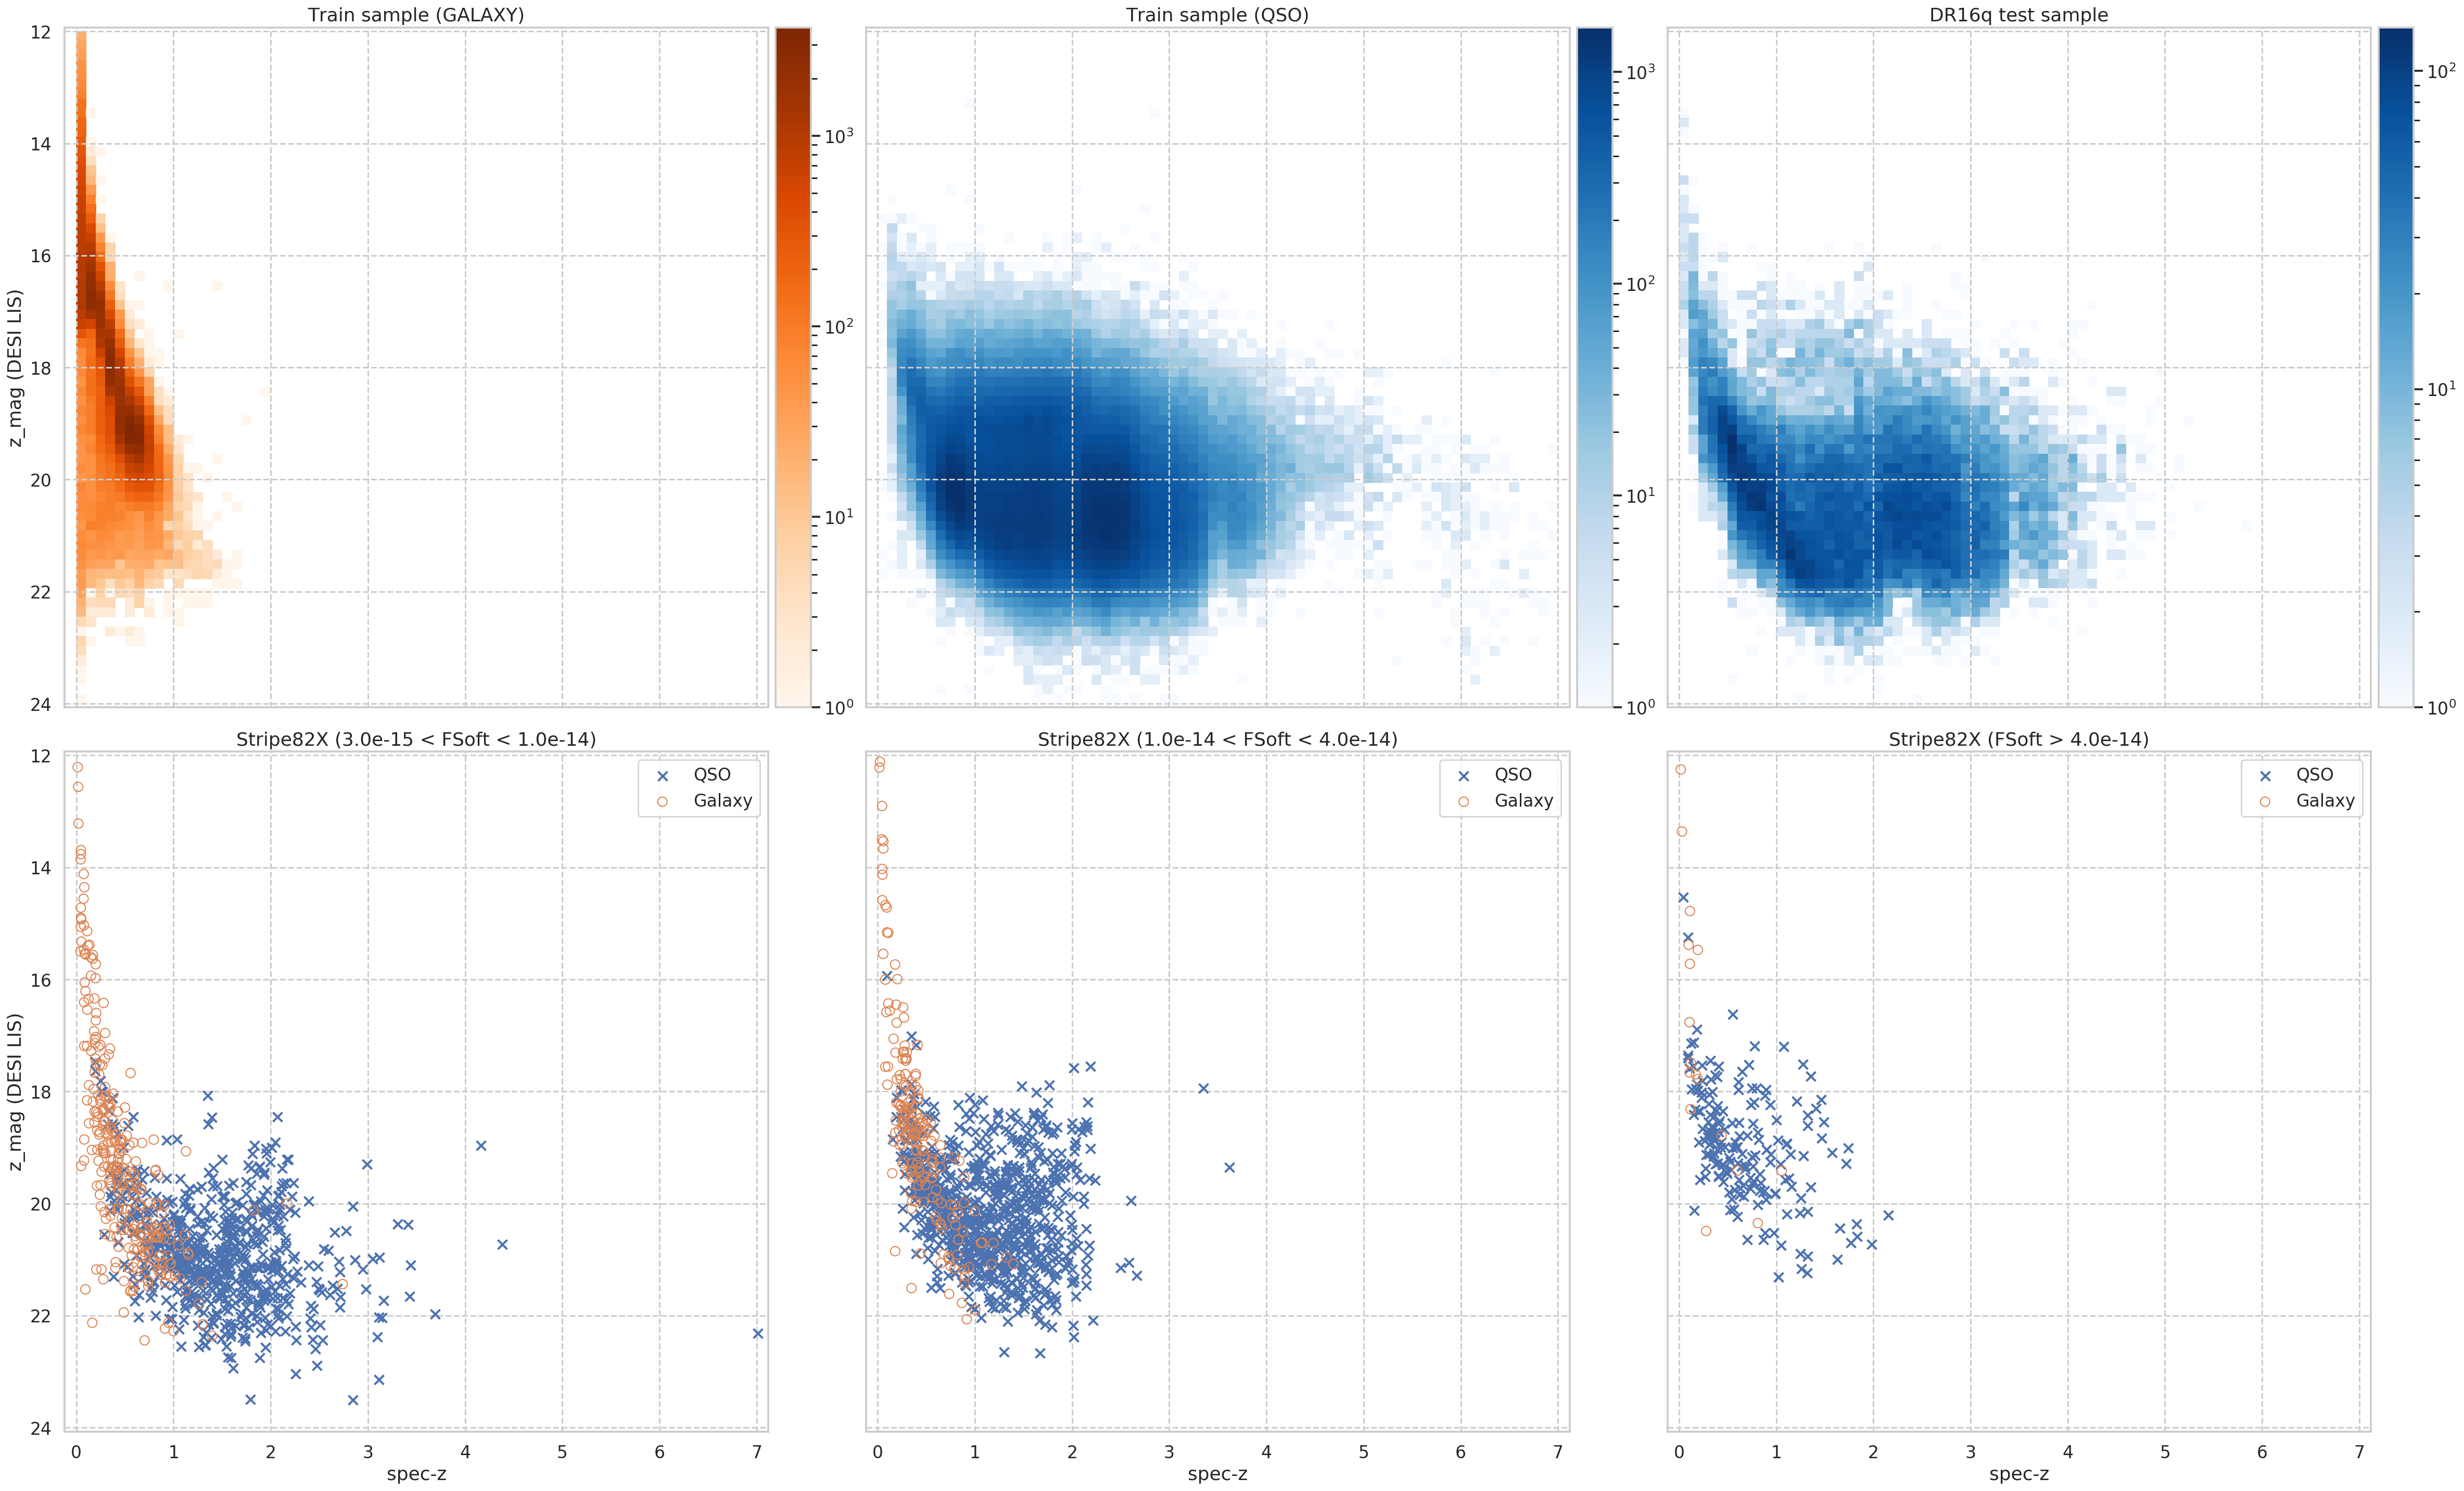
\includegraphics[width=0.95\linewidth]{images/data-dist-ab-upsidedown.png}
    \caption{The distributions of the objects in the used samples. The abscissa axis is the spectral redshift, the ordinate axis is the value \eqref{eq:mag_ab} in the $z$ filter. The upper line of the graphs, from left to right, is the distributions of galaxies and quasars in the training sample and the test sample of SDSS DR16q quasars.  The bottom line of the graphs is the distribution of Stripe82X objects with different X-ray fluxes. Orange circles show galaxies, blue crosses show quasars.}
    \label{fig:data_distribution}
\end{figure*}

% ===============================================================================
% ===============================================================================
% ===============================================================================

\section{The algorithm}

\subsection{Probabilistic regression}
To formulate a probabilistic regression problem, consider a probabilistic formulation of the regression problem. Let \(X\) be the set of object descriptions (feature space), \(Y\) be the target variable definition area. Let represent objects and target variable as random variables \(\xi : \Omega \rightarrow X, \eta : \Omega \rightarrow Y \). Then the process generating the data will be represented as a joint distribution \((\xi, \eta) \sim p(x, y)\). Let the training sample be given \(\mathcal{D}_n = (X_i, y_i)_{i=1}^n \sim p(x,y)\). Under the condition of homoscedasticity and normal distribution of errors on predictors, the regression problem is to construct an estimate of the conditional mean
\begin{equation}\label{eq:regr_classic}
     \hat{y} = \mathbb{E}[\eta | \xi = x] = \int_Y y ~ \hat{p}(y|x) ~ dy
\end{equation}

In the photometric redshift prediction problem, the errors are heteroscedastic. Moreover, the predictors are insufficiently informative (an example is to distinguish a red dwarf and a distant quasar by photometry), which generates multimodal predictive distributions $\hat{p}(y|x)$ and the estimate of the mean will be inadequate. Moreover, it is necessary to calculate confidence intervals. Therefore, it is necessary to construct a complete distribution $\hat{p}(y|x)$ for each object $x$.

Thus, the task of constructing a probabilistic regression is to train the operator \(\hat{\eta} : X \rightarrow \mathcal{P} \subset L^2\)
\begin{equation}
    \hat{\eta}(x) = \hat{p}(y|x) \in \mathcal{P},
\end{equation}
where \(\mathcal{P}\) is the set of bounded functions satisfying the properties of the probability density function, i.e.
\begin{equation}
    \forall p \in \mathcal{P}, y \in Y, x \in X \Rightarrow p(y|x) \geq 0,
\end{equation}
\begin{equation}
    \forall p \in \mathcal{P}, x \in X \Rightarrow \exists \int_{-\infty}^{+\infty} p(y|x) dy = 1.
\end{equation}

Ideally, as the training sample size \(n\) increases, the solution \(\hat{p}(y|x)\) of the problem should converge to the density function of the original generating process \(p(x|y) = \frac{p(x,y)}{p(x)}\). However, the generating process is not explicitly known: only the training sample and the test sample, on which the quality will be evaluated, are known.

The quality criteria for probabilistic predictions -- accuracy and calibration -- are described in detail in \ref{sec:metrics}.

\subsection{Random forests for probabilistic photo-z}

\subsubsection{Random forests algorithm}
Алгоритм случайного леса для решения задач регрессии классификации был впервые описан в \citep{2001MachL..45....5B} и представляет собой ансамбль деревьев решений $\{A^j\}$, которые строятся независимость. Прогноз случайного леса получается аггрегацией прогнозов всех деревьев. Например, для задачи регрессии итоговый прогноз равен среднему прогнозов деревьев.

Каждое дерево $A^j$ строит разбиение пространства признаков $X$ на непересекающиеся подпространства $A^j_i$, которые в сумме дают все пространство, то есть
\begin{equation}
    \sum_i A^j_i = X, A^j_n \cap A^j_m = \emptyset, m \neq n.
\end{equation}

Построение модели на основе алгоритма случайного леса производится следующим образом. Пусть дана обучающая выборка размера $N$:
\begin{equation}\label{eq:train_sample}
    \mathcal{D} = (\mathcal{D}_X, \mathcal{D}_y),
\end{equation}
\begin{equation}\label{eq:train_features}
    \mathcal{D}_X = (x_{i,j})_{j=1}^M,
\end{equation}
\begin{equation}\label{eq:train_target}
    \mathcal{D}_y = (y_i),
\end{equation}
где $\mathcal{D}_X$ и $\mathcal{D}_y$ признаки и разметка объектов обучающей выборки, соответственно; $i=\overline{1, N}$. Для построения очередного дерева:
\begin{itemize}
    \item бутстрепом генерируется случайная подвыборка $\mathcal{D}^j$ обучающей выборки \eqref{eq:train_sample},
    \item при каждом разбиении в $j$-ом дереве случайно выбираются случайные $m$ признаков из \eqref{eq:train_features}, $m < M$,
    \item для очередного разбиения по заданному критерию определяются оптимальный из $m$ отобранных признаков и пороговое значение,
    \item разбиения строятся пока не исчерпается вся выборка $\mathcal{D}^j$ (дерево без ограничения глубины) или до выполнения определенного условия (в каждом листе осталось не более $n_{min} \in \Theta$ объектов или достигнута заданная высота дерева $h_{max} \in \Theta$.
\end{itemize}

Впервые для задачи вероятностной регрессии был использован в работе \cite{JMLR:v7:meinshausen06a} для точечной оценки квантилей. Построение модели заключается в обучении случайного леса с квантильной функцией потерь 
\begin{equation}\label{eq:quantile_loss}
    l(y_i, \hat{q}_{\alpha, i}) = (1-\alpha)|y_i - \hat{q}_{\alpha, i}|\mathbb{I}[y_i \leq \hat{q}_{\alpha, i}] + \alpha|y_i - \hat{q}_{\alpha, i}|\mathbb{I}[y_i > \hat{q}_{\alpha, i}],
\end{equation}
% \begin{equation}\label{eq:quantile_loss}
%     l(y_i, \hat{q}_{\alpha, i}) = \left\{\begin{array}{rcl}
%          \alpha|y_i - \hat{q}_{\alpha, i}| & y_i > \hat{q}_{\alpha, i} \\
%          (1-\alpha)|y_i - \hat{q}_{\alpha, i}| & y_i \leq \hat{q}_{\alpha, i}
%     \end{array}\right.,
% \end{equation}
где $y_i$ - истинное значение, $\hat{q}_{\alpha, i}$ - предсказанное значение квантиля заданного уровня значимости $\alpha$.

(Дописать критерии разбиения!)

В работе \ref{} проводится анализ поведения случайного леса при различных параметрах рандомизации. Функцию потерь можно разложить на 2 составляющие (так называемый Bias-Variance-Tradeoff:
\begin{equation}\label{eq:bias-variance-tradeoff}
    L = Bias + Variance,
\end{equation}.
Сами по себе деревья решений являются несмещенными $Bias = 0$, но имеют высокий Variance. Путем усреднения ансамбля прогнозов удается понизить Variance.

\subsection{Случайный лес как обобщенный метод ближайших соседей}

\subsubsection{TPZ}
(Проверить!) Для задачи прогноза photo-z впервые был применен в работе \cite{bib:tpz}. Авторы предлагают 2 варианта своего метода: режим классификации и режим регрессии. В обоих режимах область определения целевого признака разбивается на конечное количество непересекающихся интервалов $[y_j, y_{j+1}]$.

В режиме классификации вероятностный прогноз строится как набор вероятностей $\hat{p}_i$ того, что целевой признак заданного объекта принадлежит тому или иному интервалу значений:
\begin{equation}
    \hat{p}_j = \mathbb{P}(y_j \leq y_i < y_{j+1}).
\end{equation}
Для каждого интервала $[y_j, y_{j+1}]$ строится модель двуклассовой классификации на основе алгоритма случайного леса, которая предсказывает вероятность $\hat{p}_j$.

В режиме регрессии производится построение одной модели регрессии на основе алгоритма случайного леса. Оценка распределения получатся нормализацией количества объектов, прогнозы которых попали в интервалы $[y_j, y_{j+1}]$.

\subsection{Random Forests adoptation for probabilistic photo-z via Gaussian KDE}
The paper (Meshcheryakov, 2018) compares probabilistic photo-z models of optical quasars based on random forest and based on gradient boosting. The random forest without depth constraint has been adapted for probabilistic predictions by applying kernel density estimation with a Gaussian kernel
\begin{equation}\label{eq:gaussian_kernel}
    K(x) = \frac{1}{\sqrt{2\pi}} * \exp{(-\frac{1}{2} x^2)}.
\end{equation}
to the ensemble of tree forecasts. Thus, the prediction is a parametric estimate of the density of the conditional distribution:
\begin{equation}\label{eq:kde}
    \hat{p}_i (y) = \hat{p}(y|x_i) = \frac{1}{n_{trees} h}\sum_{j=1}^{n_{trees}} K(\frac{y - \hat{y^{(j)}_i}}{h}),
\end{equation}
where $h$ is the kernel width parameter.

This approach has the following theoretical interpretation: the independence and randomness of the tree construction allows us to consider the ensemble of tree predictions $\{y^j_i\}_{i=1}^{n_{trees}}$ as a random sample generated by the true distribution $p(y|x_i)$. Thus \eqref{eq:kde} is an estimate of this distribution. A schematic of the method used is shown in Figure \ref{fig:qrf_scheme}.

In contrast to the random forest, each successive tree in the gradient binning builds on the previous one, which does not allow us to apply the approach described above. Instead, the model is trained with a quantile loss function \eqref{eq:quantile_loss} for different levels of significance $\alpha$, and a set of quantiles is predicted.

Based on the results of the comparison in the paper, the random forest approach showed higher accuracy than the gradient-based boosting.

% Случайный лес \cite{bib:forests_brieman} представляет собой ансамбль деревьев, основанных на одном и том же базовом алгоритме построения дерева решений, которые строятся на случайных подвыборках одной тренировочной выборки. Каждое дерево \(A^j\) задает разбиение признакового пространства \(X\) на не пересекающиеся прямоугольные подпространства \(A^j_i\), соответствующие листьям дерева, то есть
% \begin{equation}
%     X = \bigcup_i {A^j_i}; A^j_n \cap A^j_m = \emptyset, n \neq m.
% \end{equation}
% При этом каждое дерево содержит в себе некоторую случайность построения, которая контролируется вектором гиперпараметров случайного леса \(\Theta\). Например, \(\Theta\) может задавать, по какому признаку и по какому диапазону его значений будет разбиваться очередной узел. Очень важным, что будет показано ниже, является параметр, контролирующий разбиение обучающей выборки на случайные подвыборки для построения деревьев. Таким образом, деревья, входящие в случайный лес получаются разными. Для получения финального прогноза прогнозы всех деревьев усредняются, т.е., обозначив случайный лес как ансамбль деревьев \(\mathbb{V}_T = \{A^j, 1 \leq j \leq T\}\), можно записать в виде формулы
% \begin{equation}
%     \hat{\eta}_{n, \mathbb{V}_T}(x) = \frac{1}{T} \sum_{j=1}^T \hat\eta_{n, A^j}(x),
% \end{equation}
% где \(\hat\eta_{n, A^j}(x)\) - прогноз дерева \(A^j\).

% Впервые для задачи вероятностной регрессии был использован в работе Meinshausen, 2006 \cite{bib:forests_meinshausen} для точечной оценки квантилей. Построение модели заключается в обучении случайного леса с квантильной функцией потерь 
% \begin{equation}
%     l(y_i, \hat{y}_{\alpha, i}) = (1-\alpha)|y_i - \hat{y}_{\alpha, i}|\mathbb{I}[y \leq \hat{y}_{\alpha, i}] + \alpha|y_i - \hat{y}_{\alpha, i}|\mathbb{I}[y > \hat{y}_{\alpha, i}],
% \end{equation}
% где \(y_i\) - истинное значение, \(\hat{y}_{\alpha, i}\) - предсказанное значений целевой переменной.

% % Для задачи прогноза photo-z впервые был применен в работе \cite{bib:tpz}, где вероятностный прогноз строится как набор вероятностей того, что целевой признак заданного объекта принадлежит тому или иному интервалу значений. В работе \cite{bib:mesch} вероятностный прогноз представляет собой непрерывную функцию плотности вероятности, полученную применением ядерной оценки плотности к ансамблю прогнозов деревьев. Важно заметить, что в обоих алгоритмах используются леса, без ограничения глубины, т.е. когда в каждом листе каждого дерева находится один и только один элемент тренировочной выборки. 

% \subsection{Random forest adoptation for probabilistic predictions}
% Our aim was to estimate conditional redshift distribution $p(z|x)$ for each target object with photometric features $x$.
% We use Random Forest (RF) model, \citep{2001MachL..45....5B,JMLR:v7:meinshausen06a}, which is considered by many authors among the most accurate ML algorithms for photo-z measurements of galaxies \citep{2020MNRAS.499.1587S,2020arXiv200912112E} and X-ray quasars \citep{2018AstL...44..735M}. We used RF ensemble predictions in combination with gaussian Kernel Density Estimation (gKDE), to obtain $p(z|x)$. RF+gKDE model allows one to calculate photo-z point estimate $\hat{z}_{ph} = \arg\max_z p(z|x)$, confidence intervals, and $zConf = \int_{\delta z_{norm} < 0.06} p(z|x)~dz$.

% At the prediction stage we take into account uncertainties in photometric fluxes of the target object, by perturbing  fluxes (according to given uncertainties) for each regression tree in the forest

\begin{figure}
    \centering
    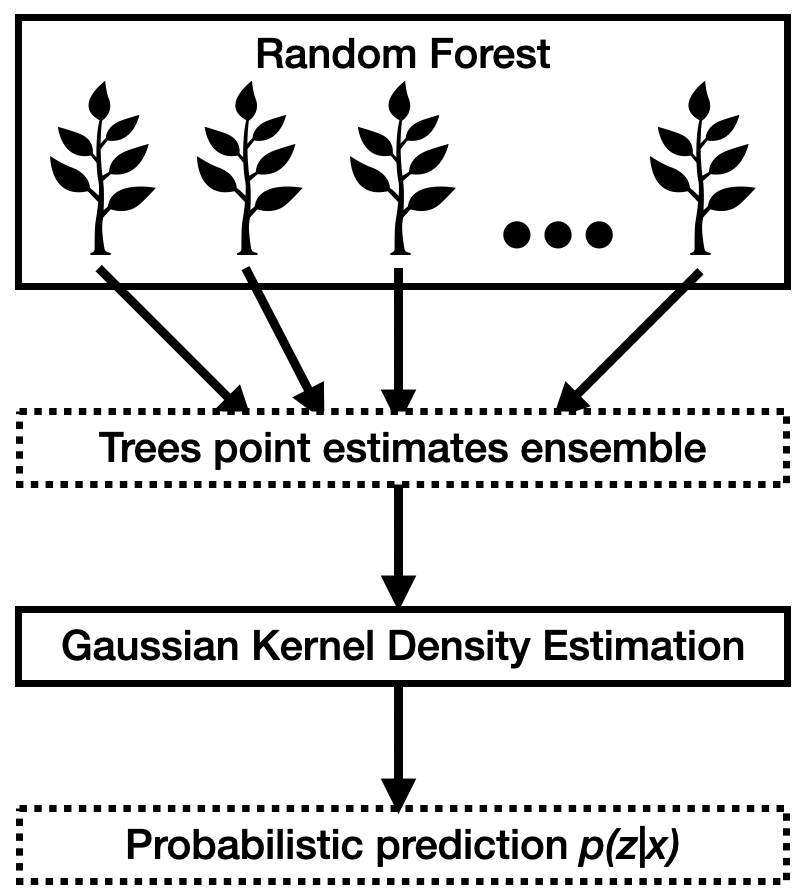
\includegraphics[width=0.95\linewidth]{images/qrf.png}
    \caption{Schematic of the random forest algorithm used, adapted to obtain probabilistic forecasts photo-z.}
    \label{fig:qrf_scheme}
\end{figure}

\section{Metrics}\label{sec:metrics}

Probabilistic predictions have 2 quality criteria -- accuracy of point predictions and calibration (matching the predicted distribution to the real one).

This section describes forecast quality metrics. Section \ref{sec:point-metrics} describes point forecast metrics, section \ref{sec:calibration-metrics} describes confidence interval and full probability forecasts calibration metrics. The \ref{sec:quality-confllict} section provides a justification for the conflict of accuracy and calibration.

\subsection{Point-estimates metrics}\label{sec:point-metrics}

To evaluate the quality of the photo-z point forecasts obtained from the probabilistic forecast, we use 2 metrics standard for the photo-z forecast problem:
\begin{itemize}
    \item normalized median absolute deviation \begin{equation}\label{eq:nmad}
        NMAD = 1.4826 \times median(|\delta z_{norm,i}|)
    \end{equation}
    \item and catastrophic outliers fraction \begin{equation}\label{eq:n015}
        n_{>0.15} = \frac{\#\{i = \overline{1, N} | \delta z_{norm, i} > 0.15\}}{N};
    \end{equation}
\end{itemize}
where \(N\) is the sample size, and the prediction error \begin{equation}\label{eq:dznorm}
    \delta z_{norm,i} = \frac{\Delta z_i}{1+z_{spec,i}} = \frac{\hat{z}_{ph,i} - z_{spec,i}}{1+z_{spec,i}}.
\end{equation}

In addition, the reliability of the prediction zConf is computed: \begin{equation}\label{eq:zconf}
    zConf = \int_{\delta z_{norm} < 0.06} p(z|x)~dz
\end{equation}

\subsection{Calibration metrics}\label{sec:calibration-metrics}

Calibration metrics can be divided into 2 types: confidence interval calibration and distribution calibration.

To assess the quality of confidence interval calibration, the theoretical and actual confidence level of 68 percent confidence intervals can be compared:
\begin{equation}\label{eq:calpha}
    C_{\alpha} = \frac{\#\{i = \overline{1, N} | z_{ph,i} \in CI_{\alpha, i}\}}{N}.
\end{equation}
A perfect calibration will achieve equality
\begin{equation}\label{eq:perfect-ci}
    C_{\alpha} = \alpha ~ \forall \alpha \in [0, 1]
\end{equation}

In this paper, we will evaluate the calibration of the 68 percent confidence intervals:
\begin{equation}\label{eq:c68}
    C_{68} - 0.68 = \frac{\#\{i = \overline{1, N} | z_{ph,i} \in CI_{68, i}\}}{N} - 0.68.
\end{equation}

To assess the calibration quality of distributions we can use Probability Inntegral Transform (PIT), which is calculated for each sample object by the formula
\begin{equation}\label{eq:pit}
PIT_i = \hat{F}_i(y_{true}); \hat{F}_i(y) = \int_{-\infty}^{y} \hat{p}_i(y|x) ~ dy
\end{equation}

If the distributions are perfectly calibrated, the PIT-values have a uniform distribution on the interval \([0,1]\), which allows using the PIT-value histogram or quantile plot for visual quality assessment (for a sample of qualitative predictions an even histogram is expected).

The quantile plot is, in a way, an integral histogram of the PIT values. A large number of too wide probability predictions (distributions) would entail a large number of PIT values around 0.5 and a convex histogram, which is a sign of "underconfidence" in the model. Conversely, a large number of too narrow distributions leads to a concave histogram, which is an indication of "overconfidence" in the model, with a large number of PIT values around 0 or around 1 indicating a large number of catastrophic outliers. 

In addition, we can use the Kolmogorov-Smirnov metric, which is the distance between the cumulative distribution function of the received PIT values \(F_{PIT}(x)\) (aka, the quantile plot) and the cumulative distribution function describing the ideal calibration, \(F_{ideal}(X)\) on the interval \([0,1]\):
\begin{equation}\label{eq:kspit}
    KS_{PIT} = \max_{x \in [0,1]}(F_{PIT}(x), F_{ideal}(x))
\end{equation}{}
\begin{equation}
    F_{PIT}(x) = \frac{\#[PIT_i < x, i=\overline{1,n}]}{N}; ~ F_{ideal} = x\mathbb{I}[0 < x \leq 1] + \mathbb{I}[x > 1]
\end{equation}{}

\subsection{Конфликт точности и калибровки}\label{sec:quality-conflict}
The quality criteria for probabilistic predictions -- accuracy and calibration -- cannot be achieved simultaneously. This is demonstrated by two dummy models.

Let us imagine that the true value of the target feature is returned as the prediction. It is 100\% accrurate, but the actual confidence level of the confidence intervals \eqref{eq:calpha} would be 1 for any confidence level values $\alpha$. All PIT values will also be equal 1.

On the other hand, we can present an example where the distribution of objects on the target attribute in the target sample is returned as a prediction for any object. In this case equality \eqref{eq:perfect-ci} will be achieved, and PIT-values will have uniform distribution on the interval [0, 1]. However, the accuracy of such a model would be quite mediocre.

% ===============================================================================
% ===============================================================================
% ===============================================================================

\section{Results}

Нашей целью является исследование поведения моделей, построенных на разных наборах признаков (прдробнее см. в \ref{}), в зависимости от наблюдаемых предикторов (величины в фильтрах r, z, рентгеновский поток) и от целевой величины (spec-z). Чтобы добиться лучшего разрешения (это особенно актуально для объектов на $z > 3$) мы используем метод двукратной перекрестной оценки и выборку оптических квазаров SDSS DR16q, описанную в разделе \ref{}. Эти наблюдения описаны в разделе \ref{subsec:cv2_results} и \ref{subsec:dr16_results}, соответственно.

В разделе \ref{subsec:s82x_results} такие же наблюдения на выборке рентгеновских объетов Stripe82X, описанной в разделе \ref{}. На этой же выборке мы приводим сранение с прогнозами моделей SOTA \ref{}.

\subsection{Результаты на кросс-валидации (галактики)}

\subsection{Результаты на кросс-валидации (квазары)}
В данном разделе рассматривается поведение моделей на двукратной кросс-валидации и на тестовой выборке оптических квазаров SDSS DR16q.

Описать преимущества двукратной кросс-валидации.

Для двукратной кросс-валидации тренировочная выборка была разделена на 2 части равномерно по spec-z. Контролировать равномерность разбиения необходимо в областях с небольшим количеством обучающих примеров (например, чтобы объекты на $z > 6$ были в обеих частях в одинаковой пропорции, а не попали в одну часть).

Прогнозы двукратной кросс-валидации можно рассматривать независиомо (как? почему? зачем это надо) в том смысле, что вложения не перекрываются при обучении очередной модели, таким образом модели двукратной кросс-валидации получаются независимыми, а кросс-валидационные прогнозы можно рассматривать как прогнозы на тестовой выборке.

В результате модели показали одинаковое поведение на обоих вложениях, поэтому кросс-валидационные прогнозы будут рассмотрены вместе (криво!).

\subsection{Результаты на тестовой выборке оптических квазаров}

На рисунке \ref{fig:dr16q_wo_train} приведены диаграммы рассеяния прогнозов разных моделей на тестовой выборке оптических квазаров SDSS DR16q. Напомним, что основное различие между моделями -- используемые наборы признаков. Количество тренировочных примеров меняется незначительно (подробнее сослаться на таблицу). По диаграммам видно, что  лучше остальных на далеких объектах ($spec-z > 3,5$) себя показывают модели использующие оба каталога Pan-STARRS и DESI LIS (прогнозы лежат ближе к диагонали, меньше прогнозов с низкой достоверностью). Лучше всего в среднем ($1 < spec-z < 3$) себя показывает модель, построенная на признаках всех используемых фотометрических обзоров.

Это подтверждается графиками зависимости метрик от целевой переменной (спектральное красное смещение, см. рис. \ref{fig:metrics-qso_spec-z}). Из графиков так же видно, что модель DESI LIS + WISE имеет точность примерно в два раза ниже остальных моделей. Интересно, точность моделей не имеет простой (например, монотонной), зависимости от красного смещения. На разных интервалах красного смещения точность может меняться как одновременно у всех моделей, так и только у некоторых моделей. Вот некоторые наблюдения, сделанные из графиков:

Кроме того была обнаружена зависимость между яркостью объектов и точностью моделей. Мы приводим график только в зависимости от величины $r$ (см. рис. \ref{fig:metrics-qso_z_mag}), однако аналогичные выводы верны, если рассматривать зависимость точности от других величин. Вот некоторые выводы, которые можно сделать:
\begin{itemize}
    \item точность моделей падает на слабых объектов (например, у модели Pan-STARRS до 2.5 раз).
    \item отсутствие фильтров $i$ и $y$ приводит к понижению точности прогнозов для ярких объектов (см. модели DESI LIS + WISE и Pan-STARRS + WISE).
\end{itemize}

\subsection{Stripe82X results}\label{subsec:s82x_results}

В данном разделе приведено описание результатов, полученных на выборке Stripe82X и сравнение с моделями (Ananna, Brescia \ref{}). В целом выводы о поведении моделей повторяют изложенное ранее в пункте \ref{}, поэтому здесь мы заострим внимание на сравнении с моделями других исследователей.

На рис. \ref{fig:s82x} показаны диаграммы рассеяния прогнозов для шести моделей. Можно видеть, что модель на основе четырех широких обзоров SDSS + Pan-STARRS + DESI LIS + WISE так же показвыает себя с лучшей стороны (прогнозы сильнее сгруппрированы вокруг диагонали, меньшая доля выбросов, точные прогнозы имеют бОльшую достоверность). Модель Ananna в свою очередь дает слишком высокую уверенность прогнозов: существенная доля катастрофических выбросов имеет $PDZbest \sim 1$.

\begin{figure}
    \centering
    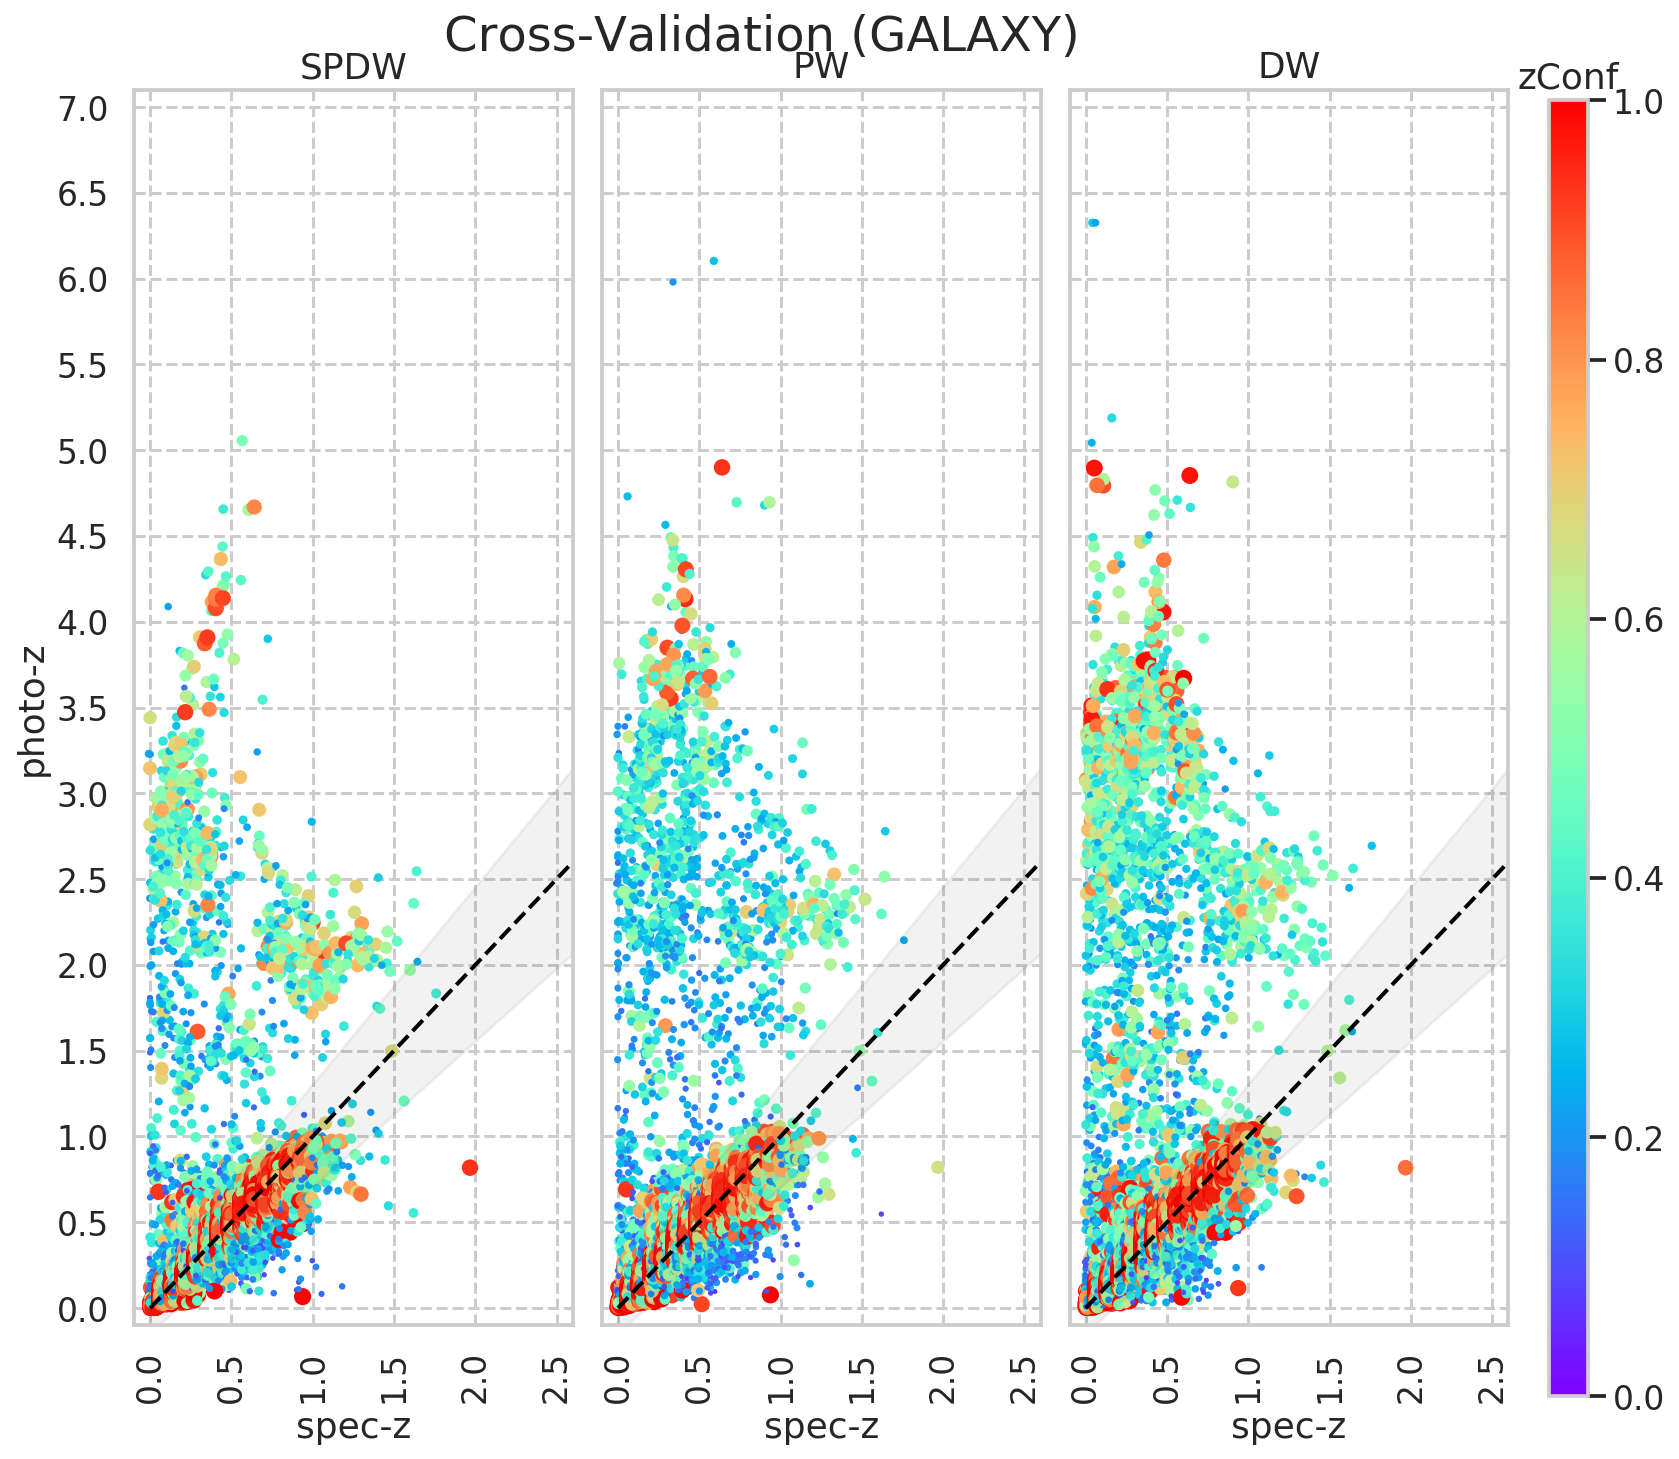
\includegraphics[width=0.9\linewidth]{images/scatterplots-cv2-gal.png}
    \caption{Scatterplots of cross-validation predictions of galaxies of three models (from left to right) -- \ref{model:spdw}, \ref{model:pw}, \ref{model:dw}. The abscissa axis shows the spectral redshift value, and the ordinate axis shows the photometric redshift prediction. The color and size of dots show the prediction reliability zConf \eqref{eq:zconf}. The gray area around the diagonal is the area of predictions that are not catastrophic emissions according to metric \eqref{eq:n015}.}
    \label{fig:metrics-cv2-gal}
\end{figure}

\begin{figure*}
    \centering
    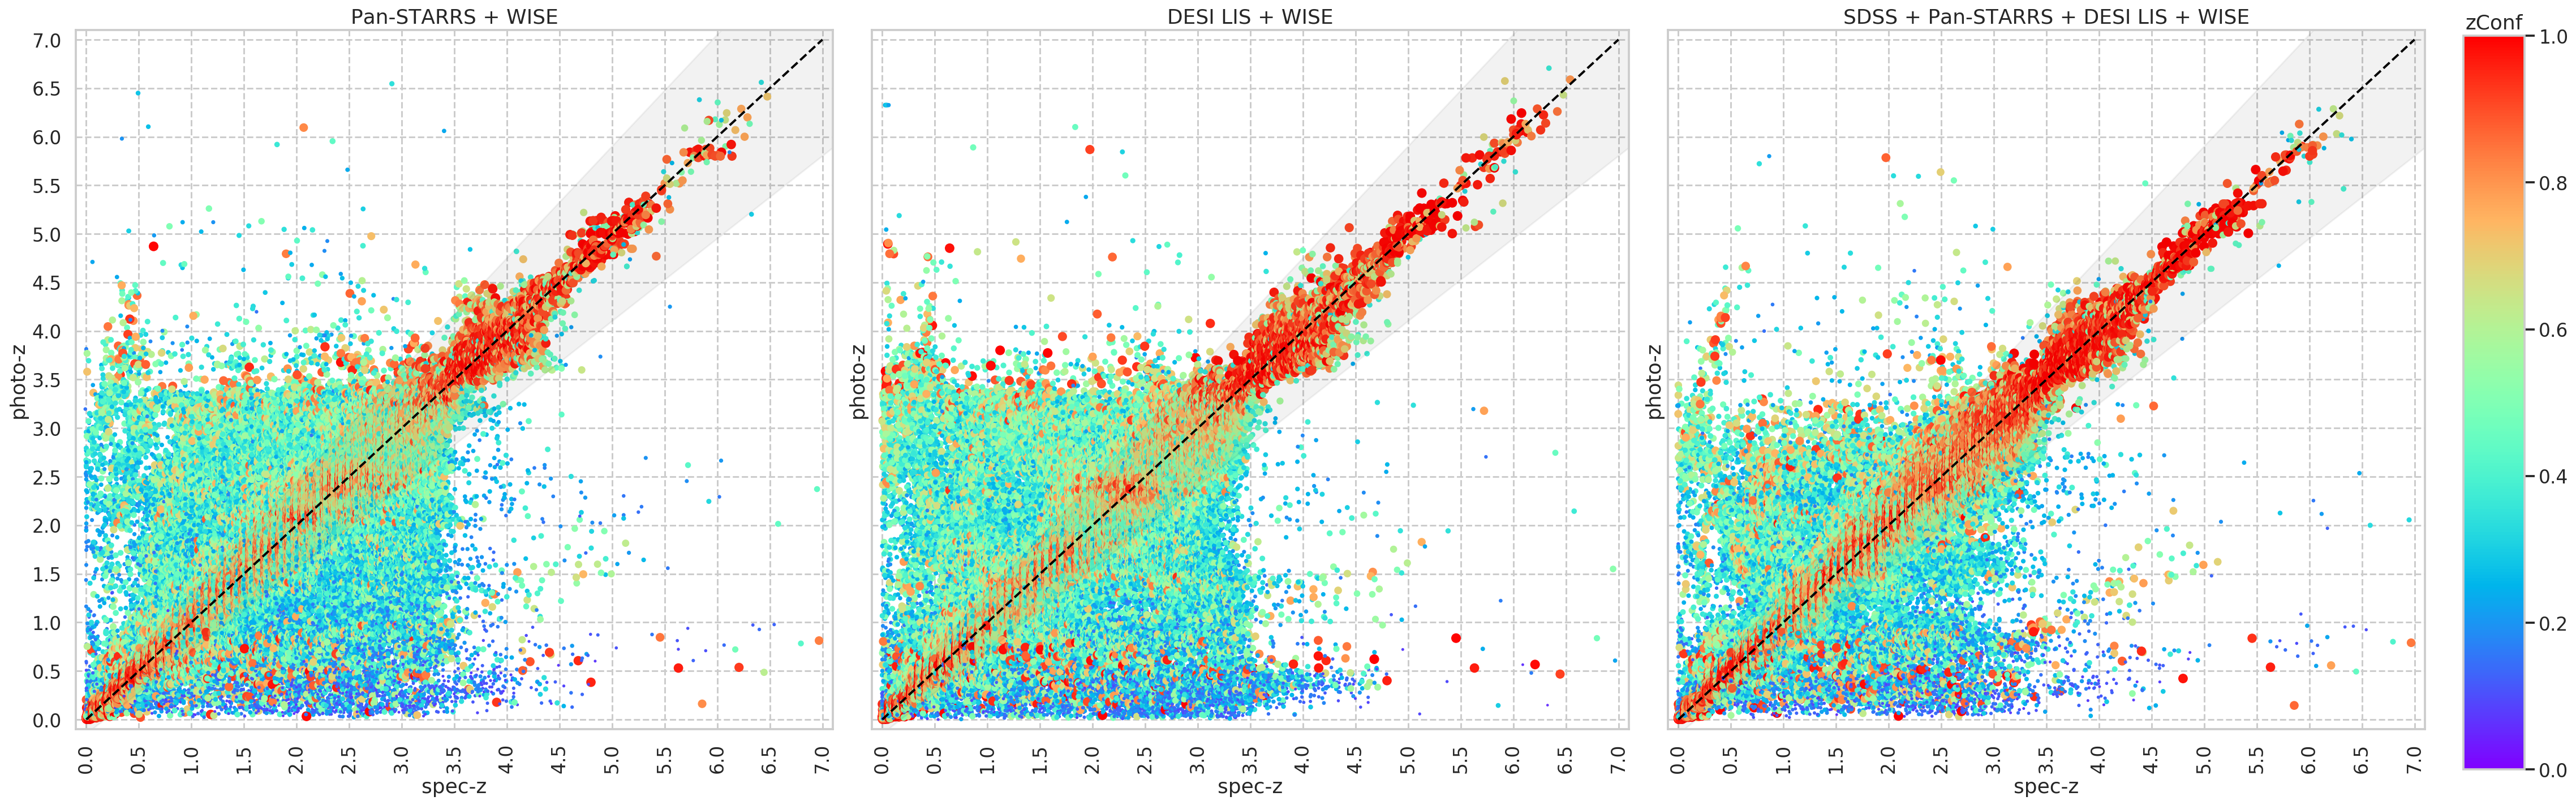
\includegraphics[width=0.9\linewidth]{images/scatterplots-cv2-total.png}
    \caption{Scatterplots of cross-validation predictions of galaxies and quasars of three models (from left to right) -- \ref{model:spdw}, \ref{model:pw}, \ref{model:dw}. The abscissa axis shows the spectral redshift value, and the ordinate axis shows the photometric redshift prediction. The color and size of dots show the prediction reliability zConf \eqref{eq:zconf}. The gray area around the diagonal is the area of predictions that are not catastrophic emissions according to metric \eqref{eq:n015}.}
    \label{fig:my_label}
\end{figure*}

\begin{figure*}
    \centering
    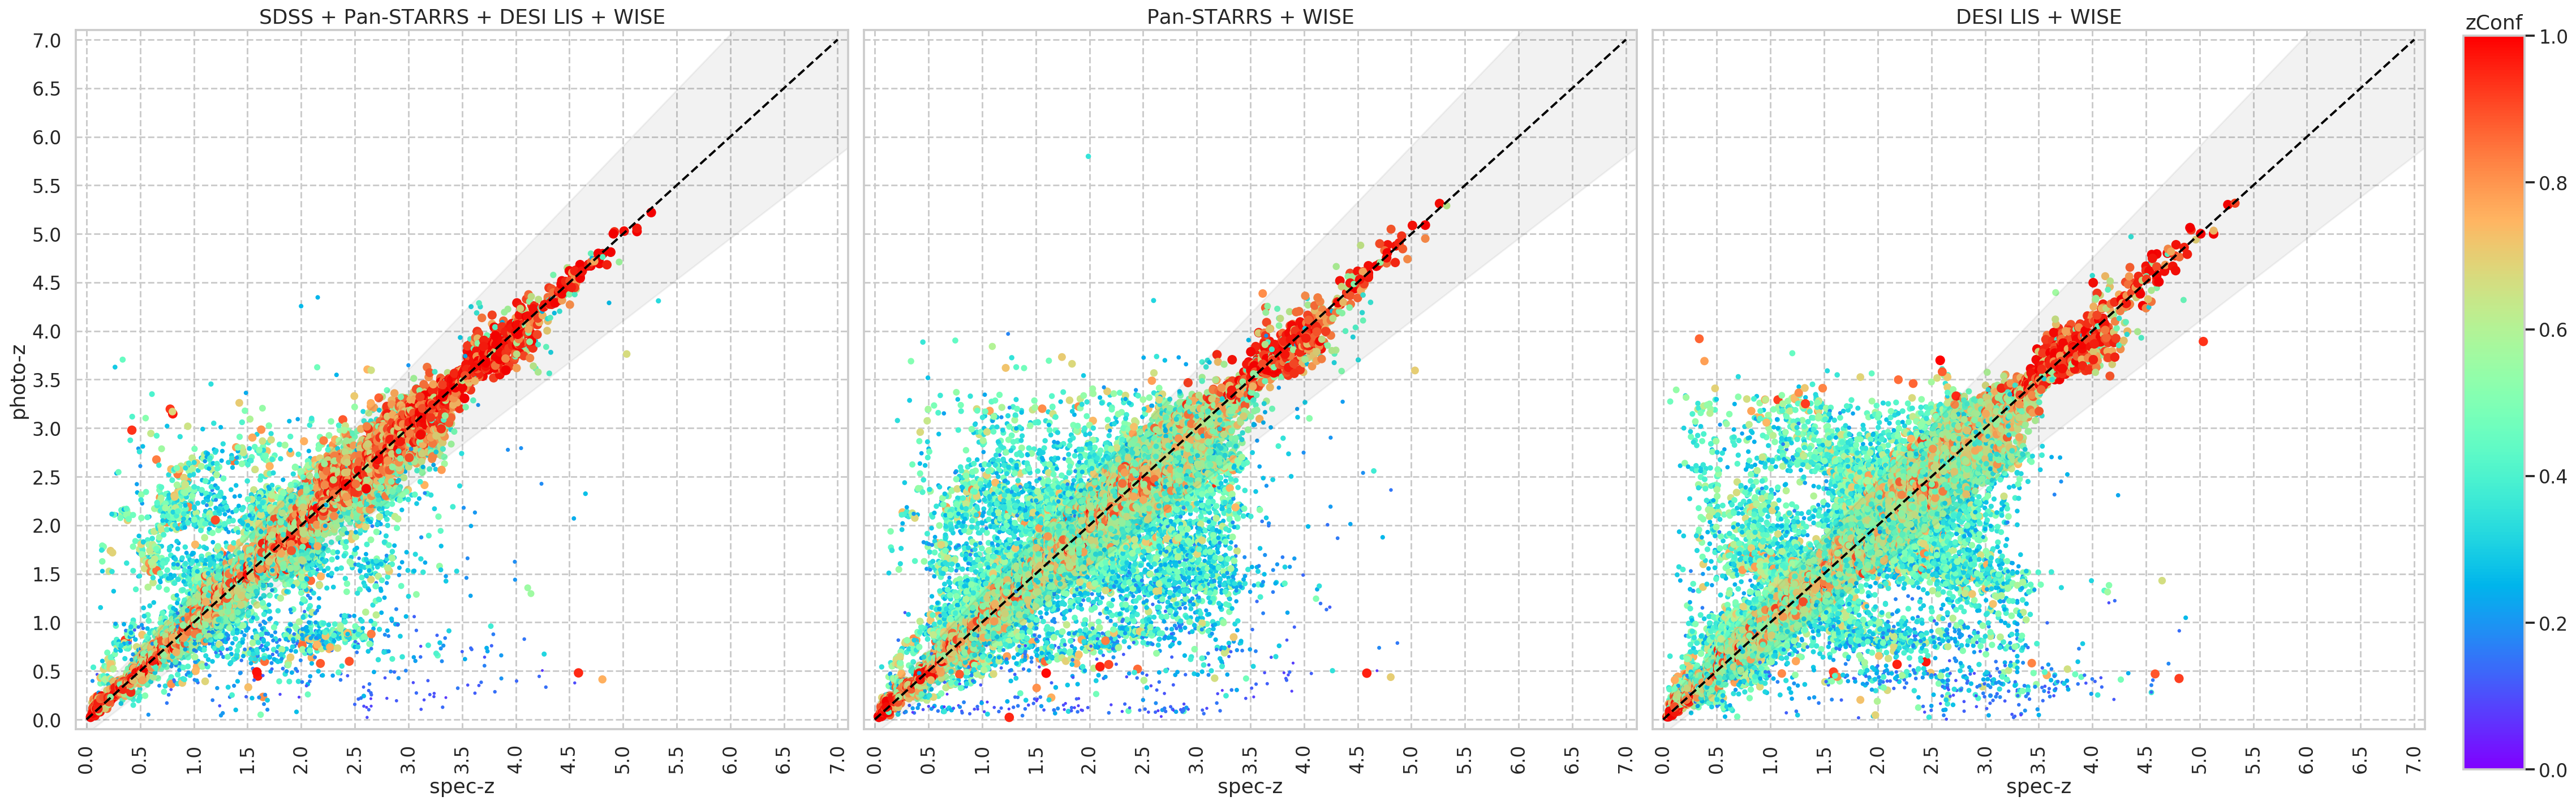
\includegraphics[width=0.9\linewidth]{images/scatterplots-dr16q-wo-train.png}
    \caption{Scatterplots of predictions on SDSS DR16 quasars test sample of three models (from left to right) -- \ref{model:spdw}, \ref{model:pw}, \ref{model:dw}. The abscissa axis shows the spectral redshift value, and the ordinate axis shows the photometric redshift prediction. The color and size of dots show the prediction reliability zConf \eqref{eq:zconf}. The gray area around the diagonal is the area of predictions that are not catastrophic emissions according to metric \eqref{eq:n015}.}
    \label{fig:dr16q_wo_train}
\end{figure*}

\begin{figure*}
    \centering
    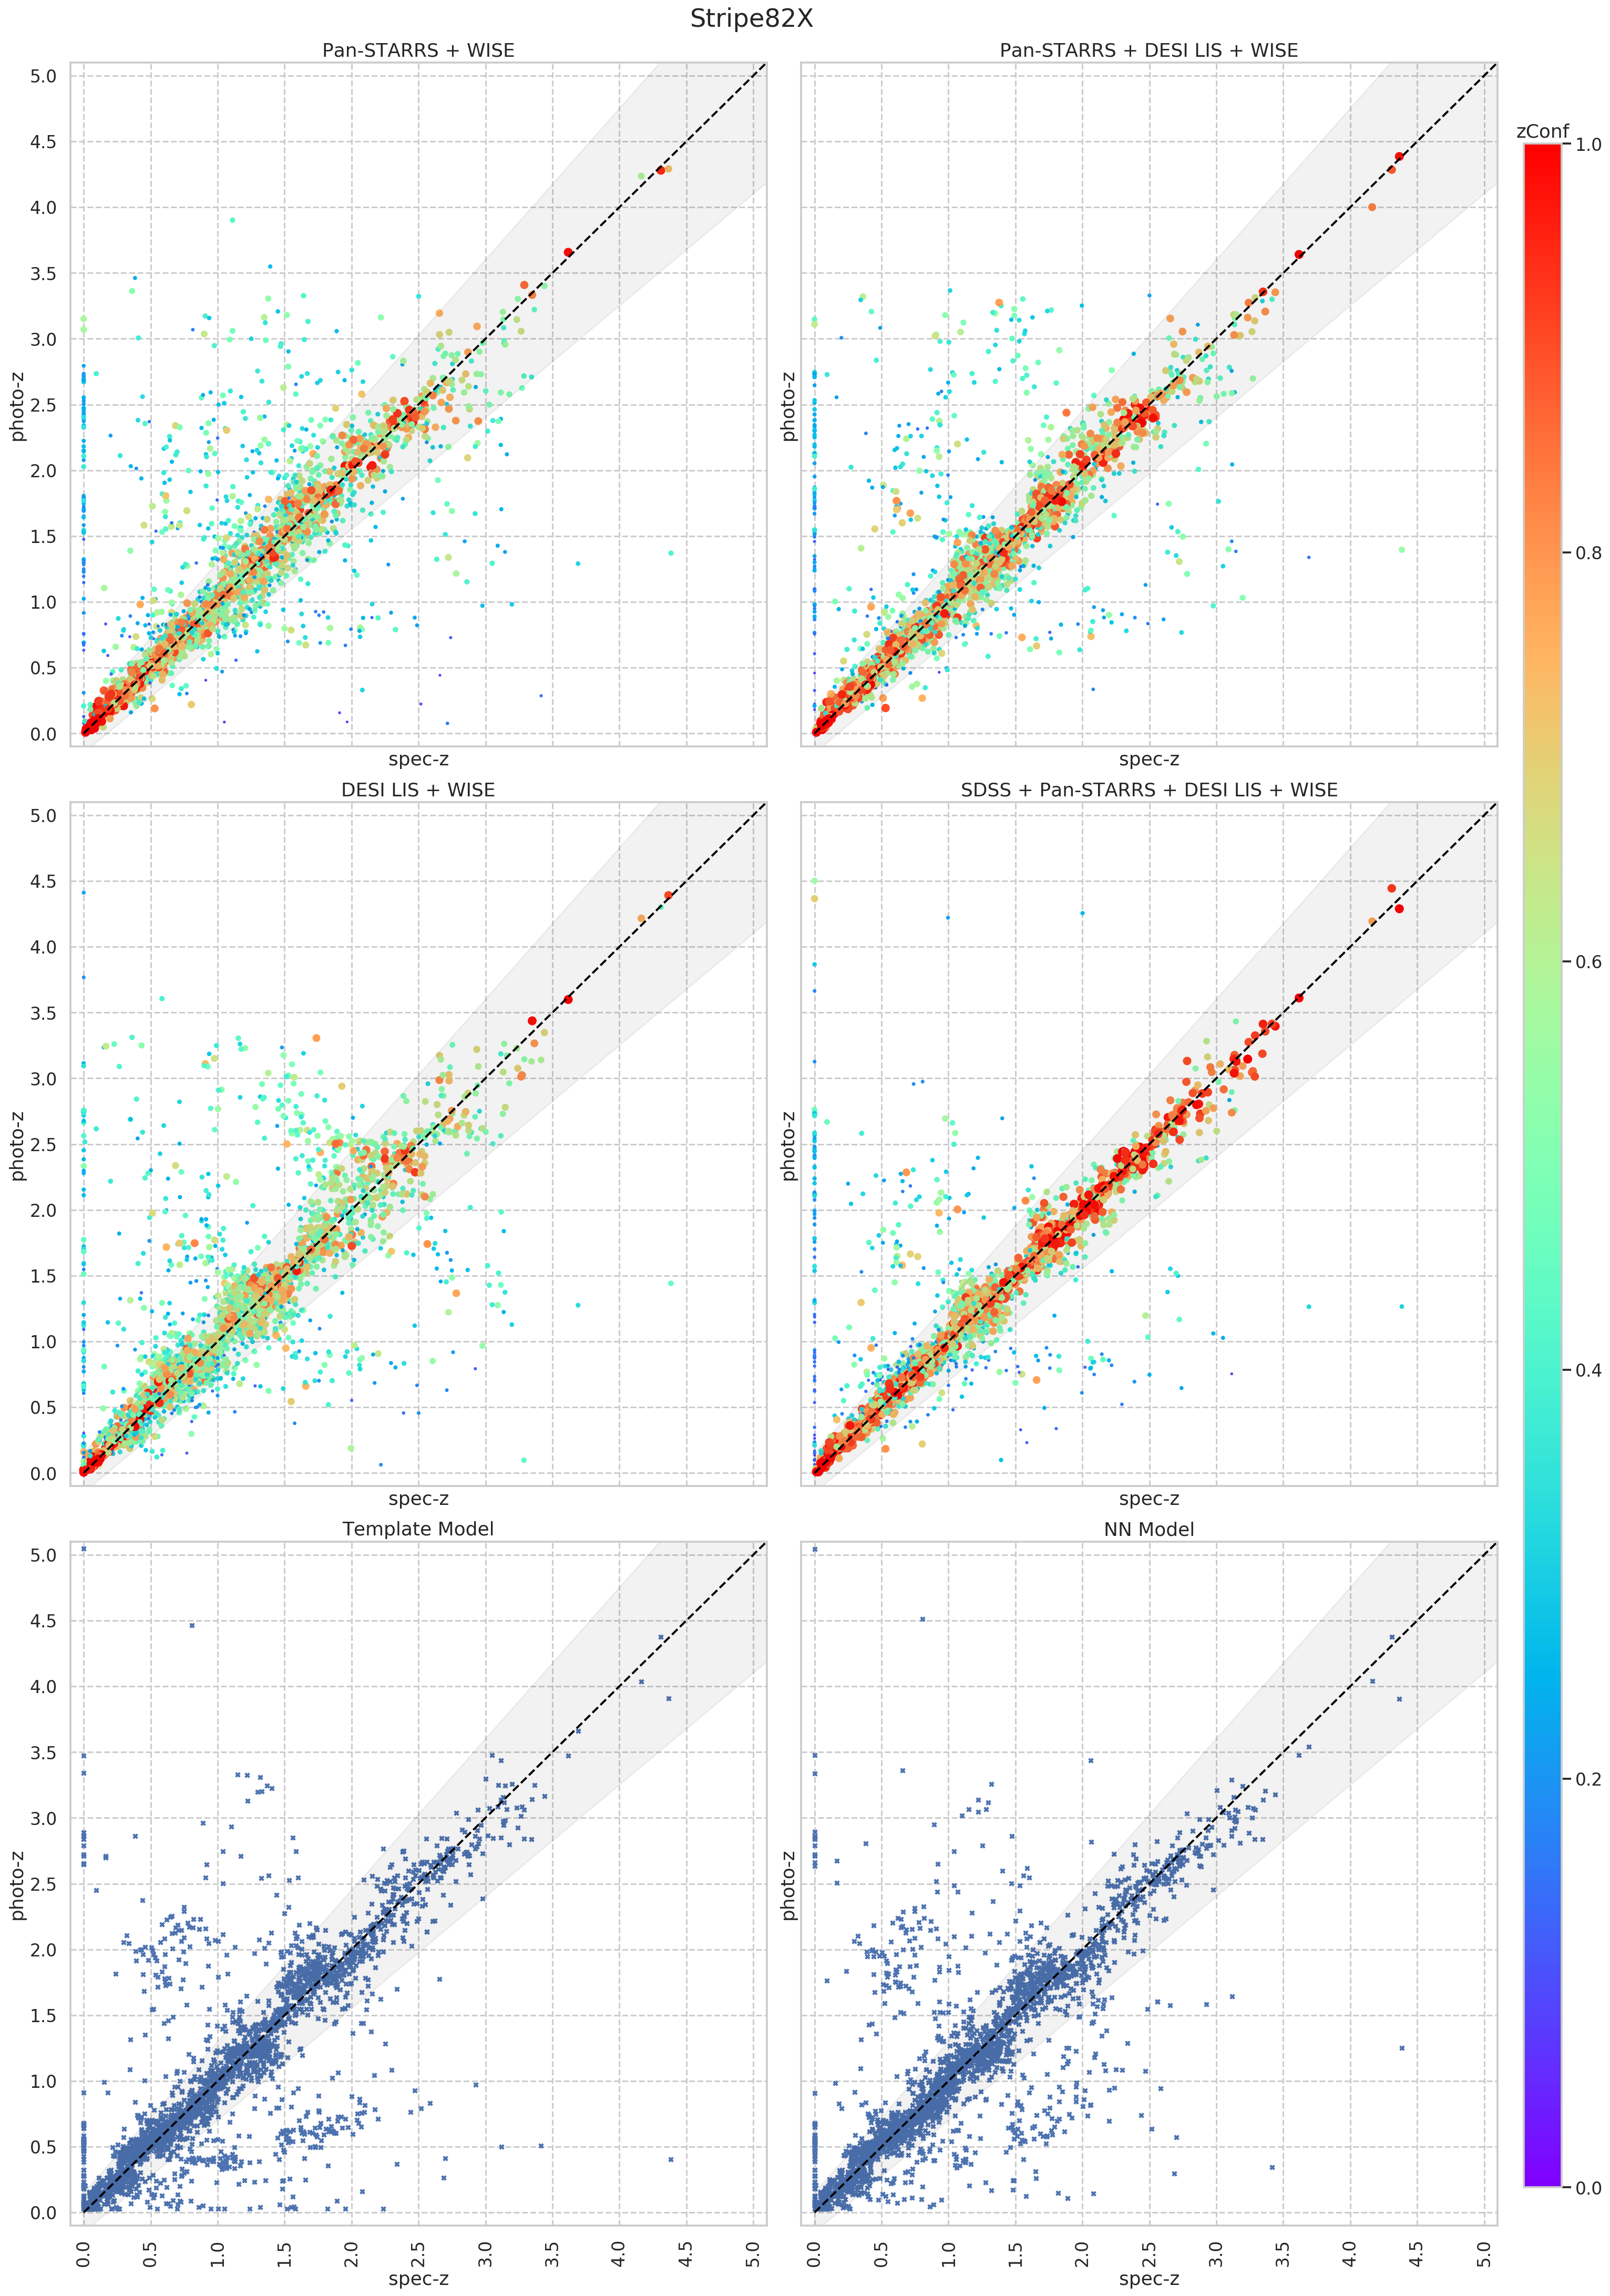
\includegraphics[width=0.9\linewidth]{images/scatterplots-stripe82x.png}
    \caption{Scatterplots of predictions on Stripe82X X-ray test sample of three models (from left to right) -- \ref{model:spdw}, \ref{model:pw}, \ref{model:dw}. The abscissa axis shows the spectral redshift value, and the ordinate axis shows the photometric redshift prediction. The color and size of dots show the prediction reliability zConf \eqref{eq:zconf}. The gray area around the diagonal is the area of predictions that are not catastrophic emissions according to metric \eqref{eq:n015}.}
    \label{fig:s82x}
\end{figure*}


\begin{figure*}
    \centering
    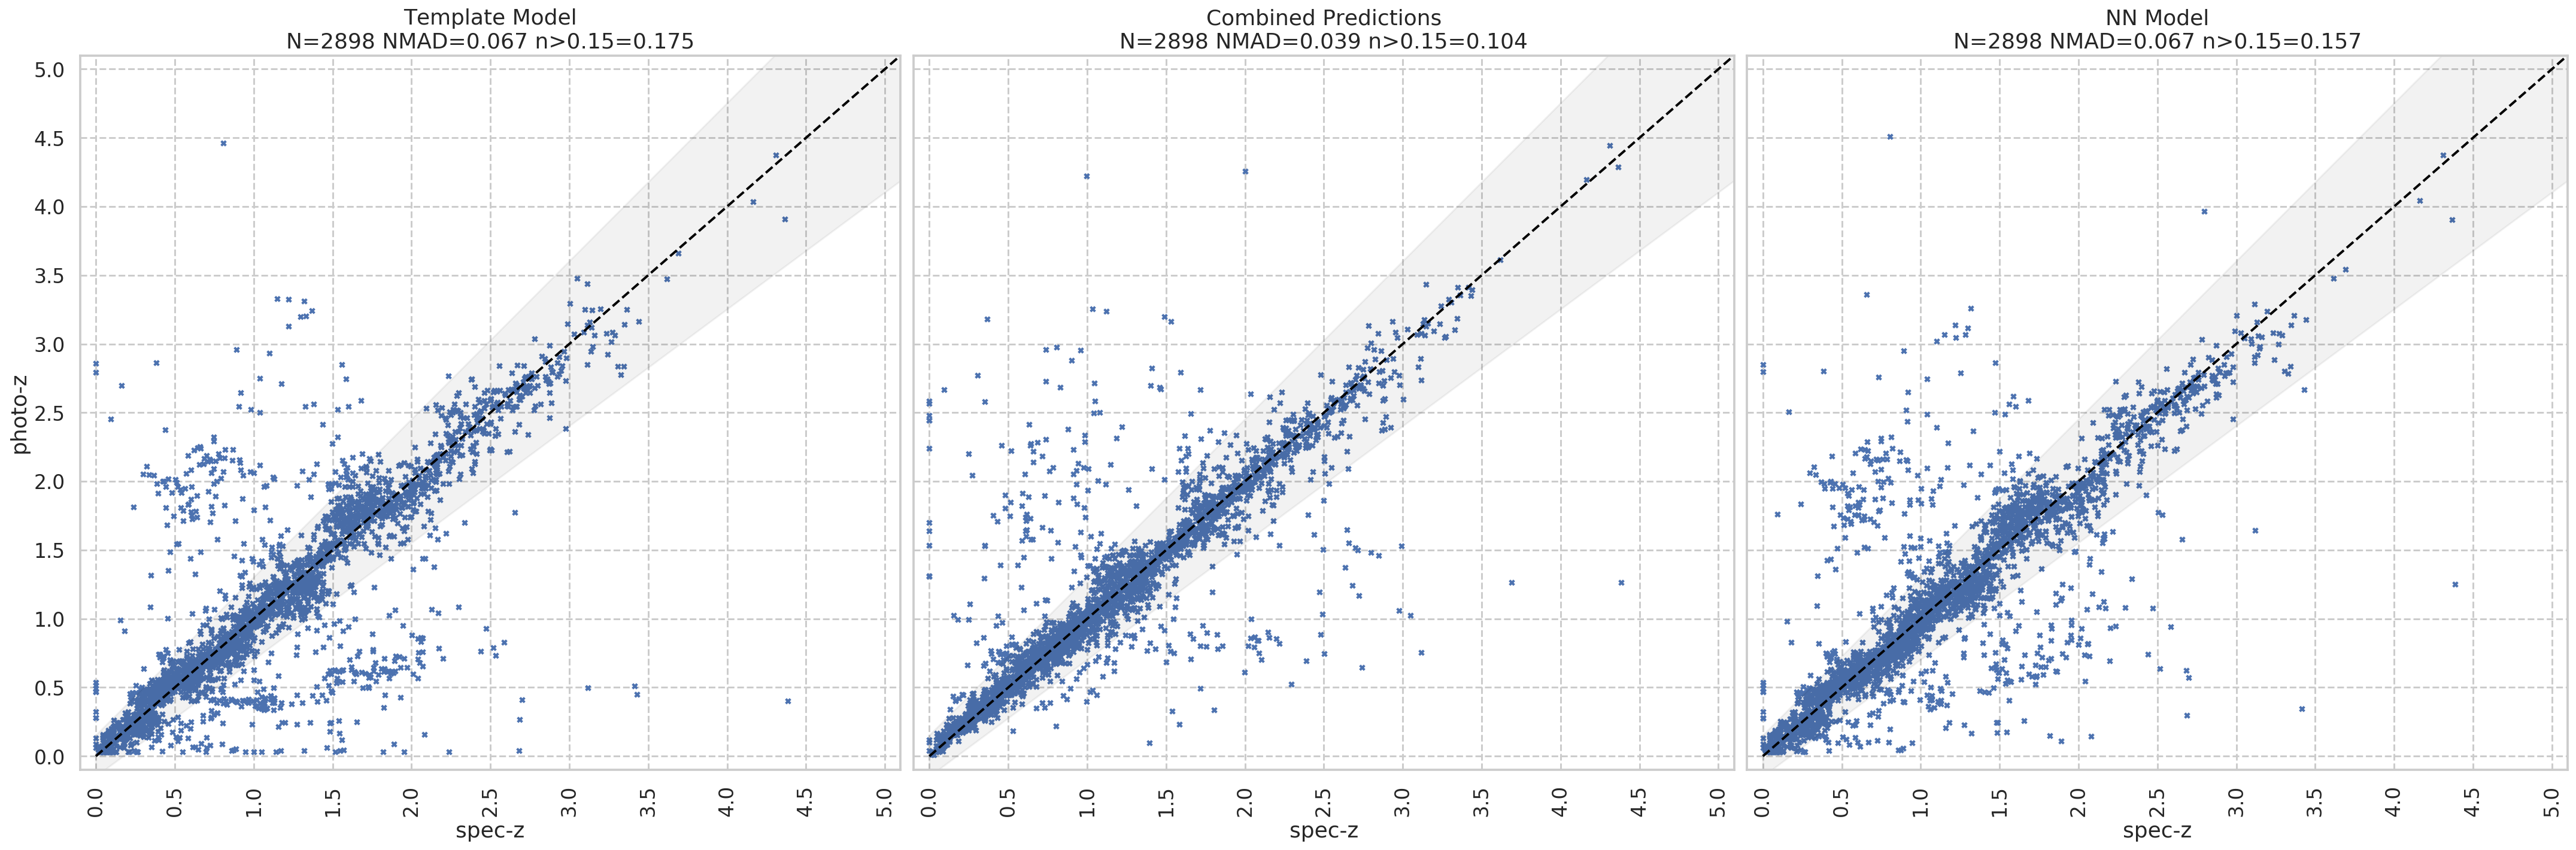
\includegraphics[width=0.9\linewidth]{images/scatterplots-stripe82x-sota-combined.png}
    \caption{Scatterplots of predictions of template model (Ananna, 2017), combined prediction of models \ref{model:pw} -- \ref{model:spdw}, neural network model (Brescia, 2019) on Stripe82X X-ray test sample (from left to right). The abscissa axis shows the spectral redshift value, and the ordinate axis shows the photometric redshift prediction. The gray area around the diagonal is the area of predictions that are not catastrophic emissions according to metric \eqref{eq:n015}.}
    \label{fig:s82x-sota35}
\end{figure*}

\begin{figure*}
    \centering
    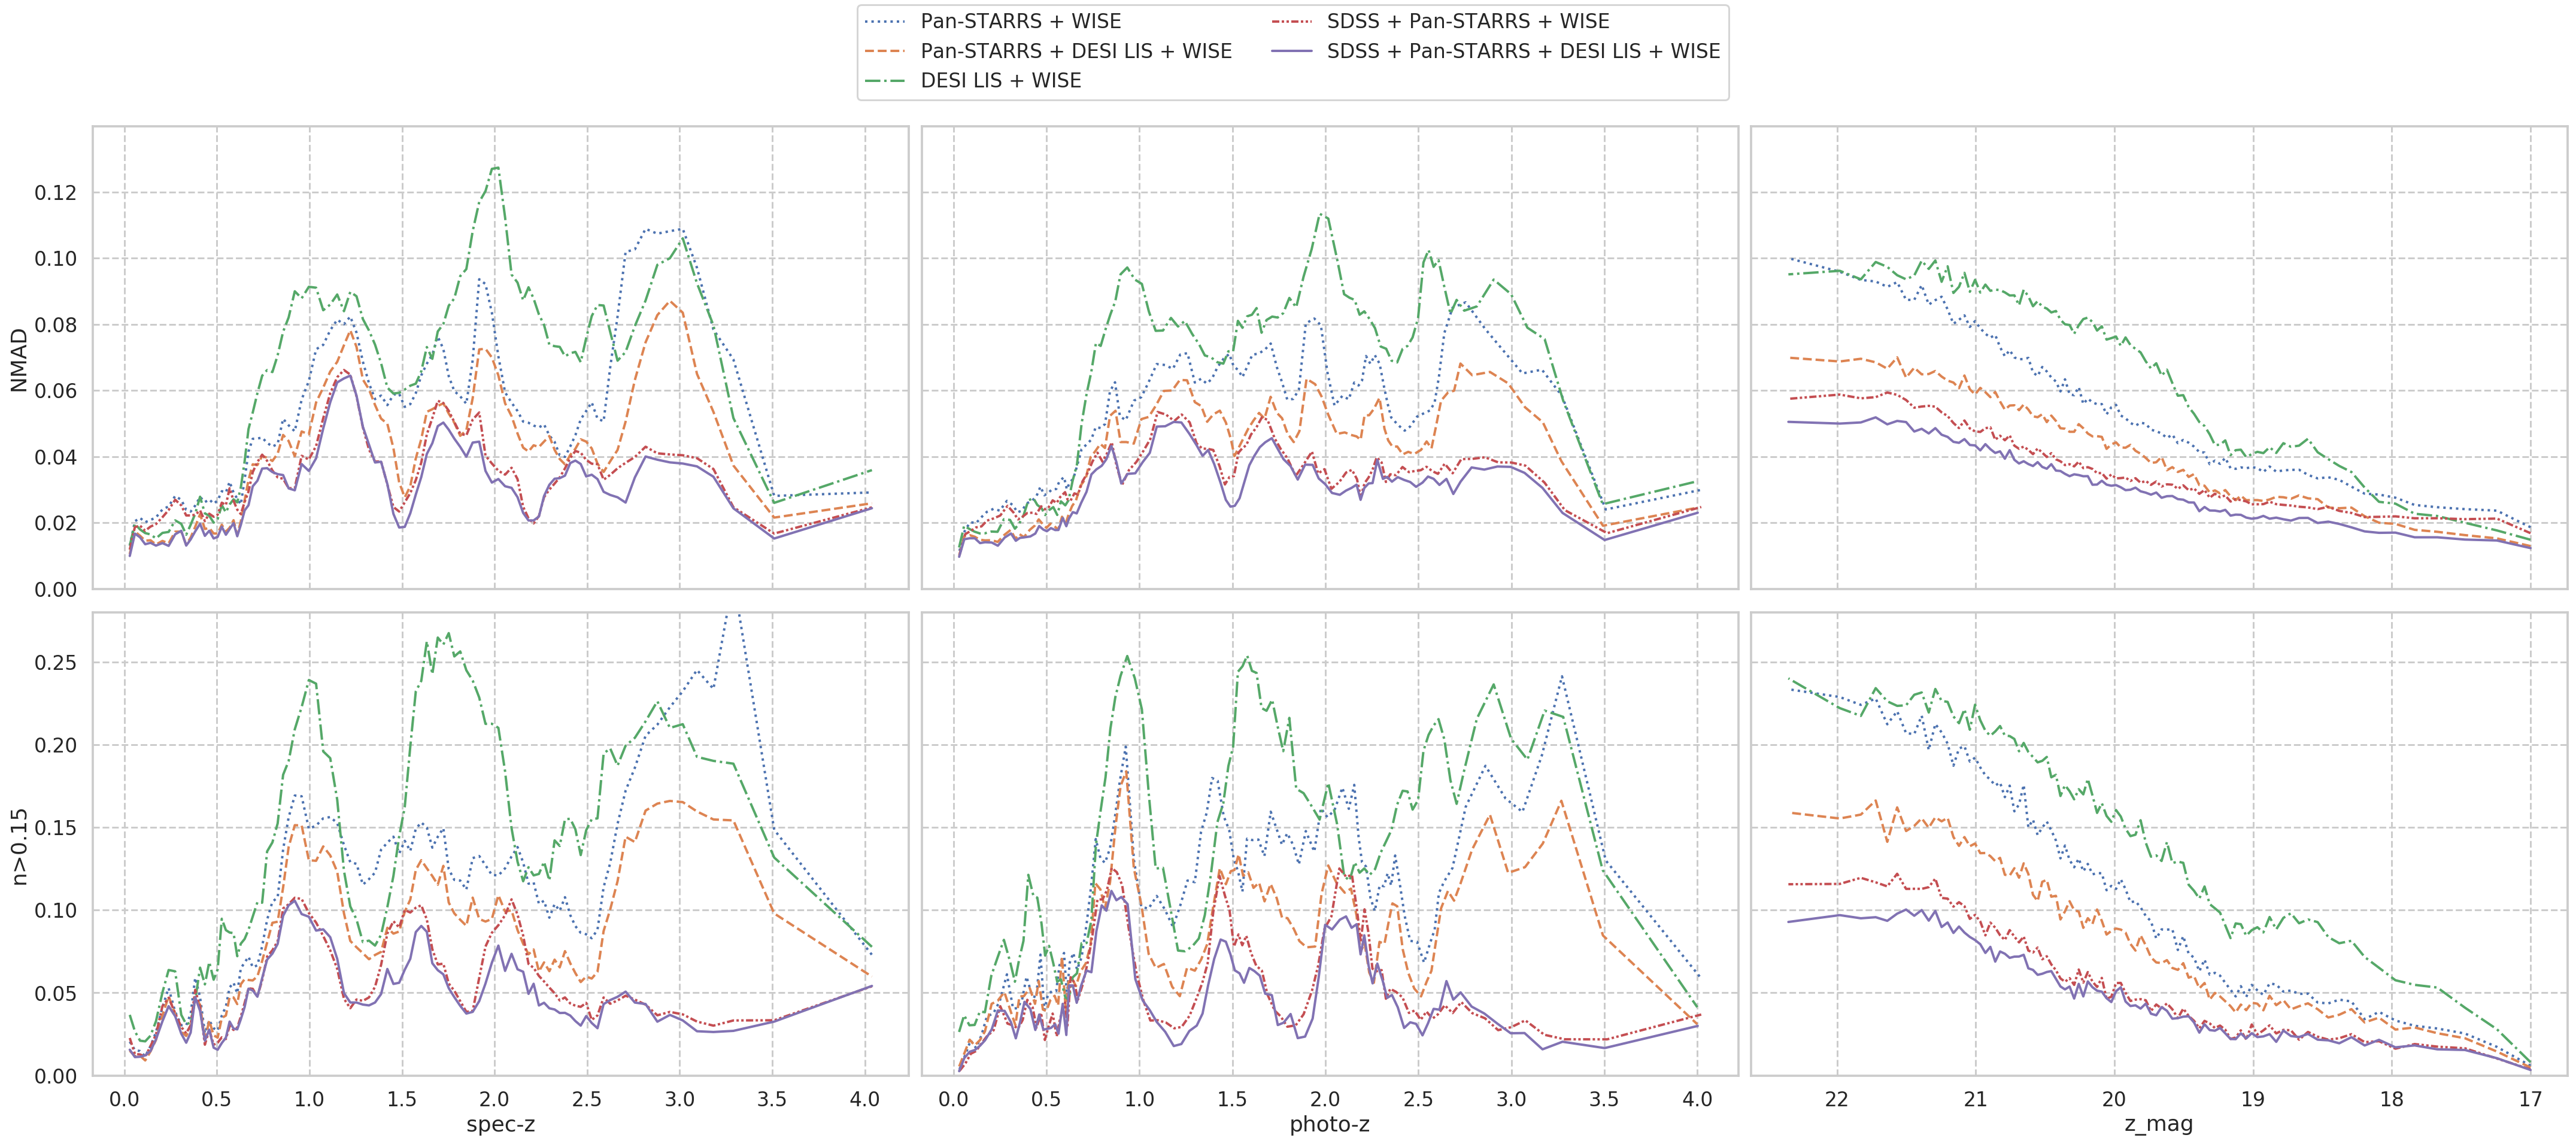
\includegraphics[width=0.9\linewidth]{images/metrics-cv2-ab-mini.png}
    \caption{Plots of NMAD \eqref{eq:nmad} (upper line of plots) and the fraction of catastrophic outliers \eqref{eq:n015} (lower line of plots) metrics as a function of (from left to right) spectral redshift value, photometric redshift prediction value, and stellar magnitude in the filter z) of cross-validation predictions. The solid line shows model \ref{model:spdw}, the dot line shows model \ref{model:pw}, the dashed line shows model \ref{model:pdw}, the dash-dot line shows model \ref{model:dw}, and dash-dot-dot line shows model \ref{model:spw}.}
    \label{fig:metrics-cv2-ab}
\end{figure*}

\begin{figure*}
    \centering
    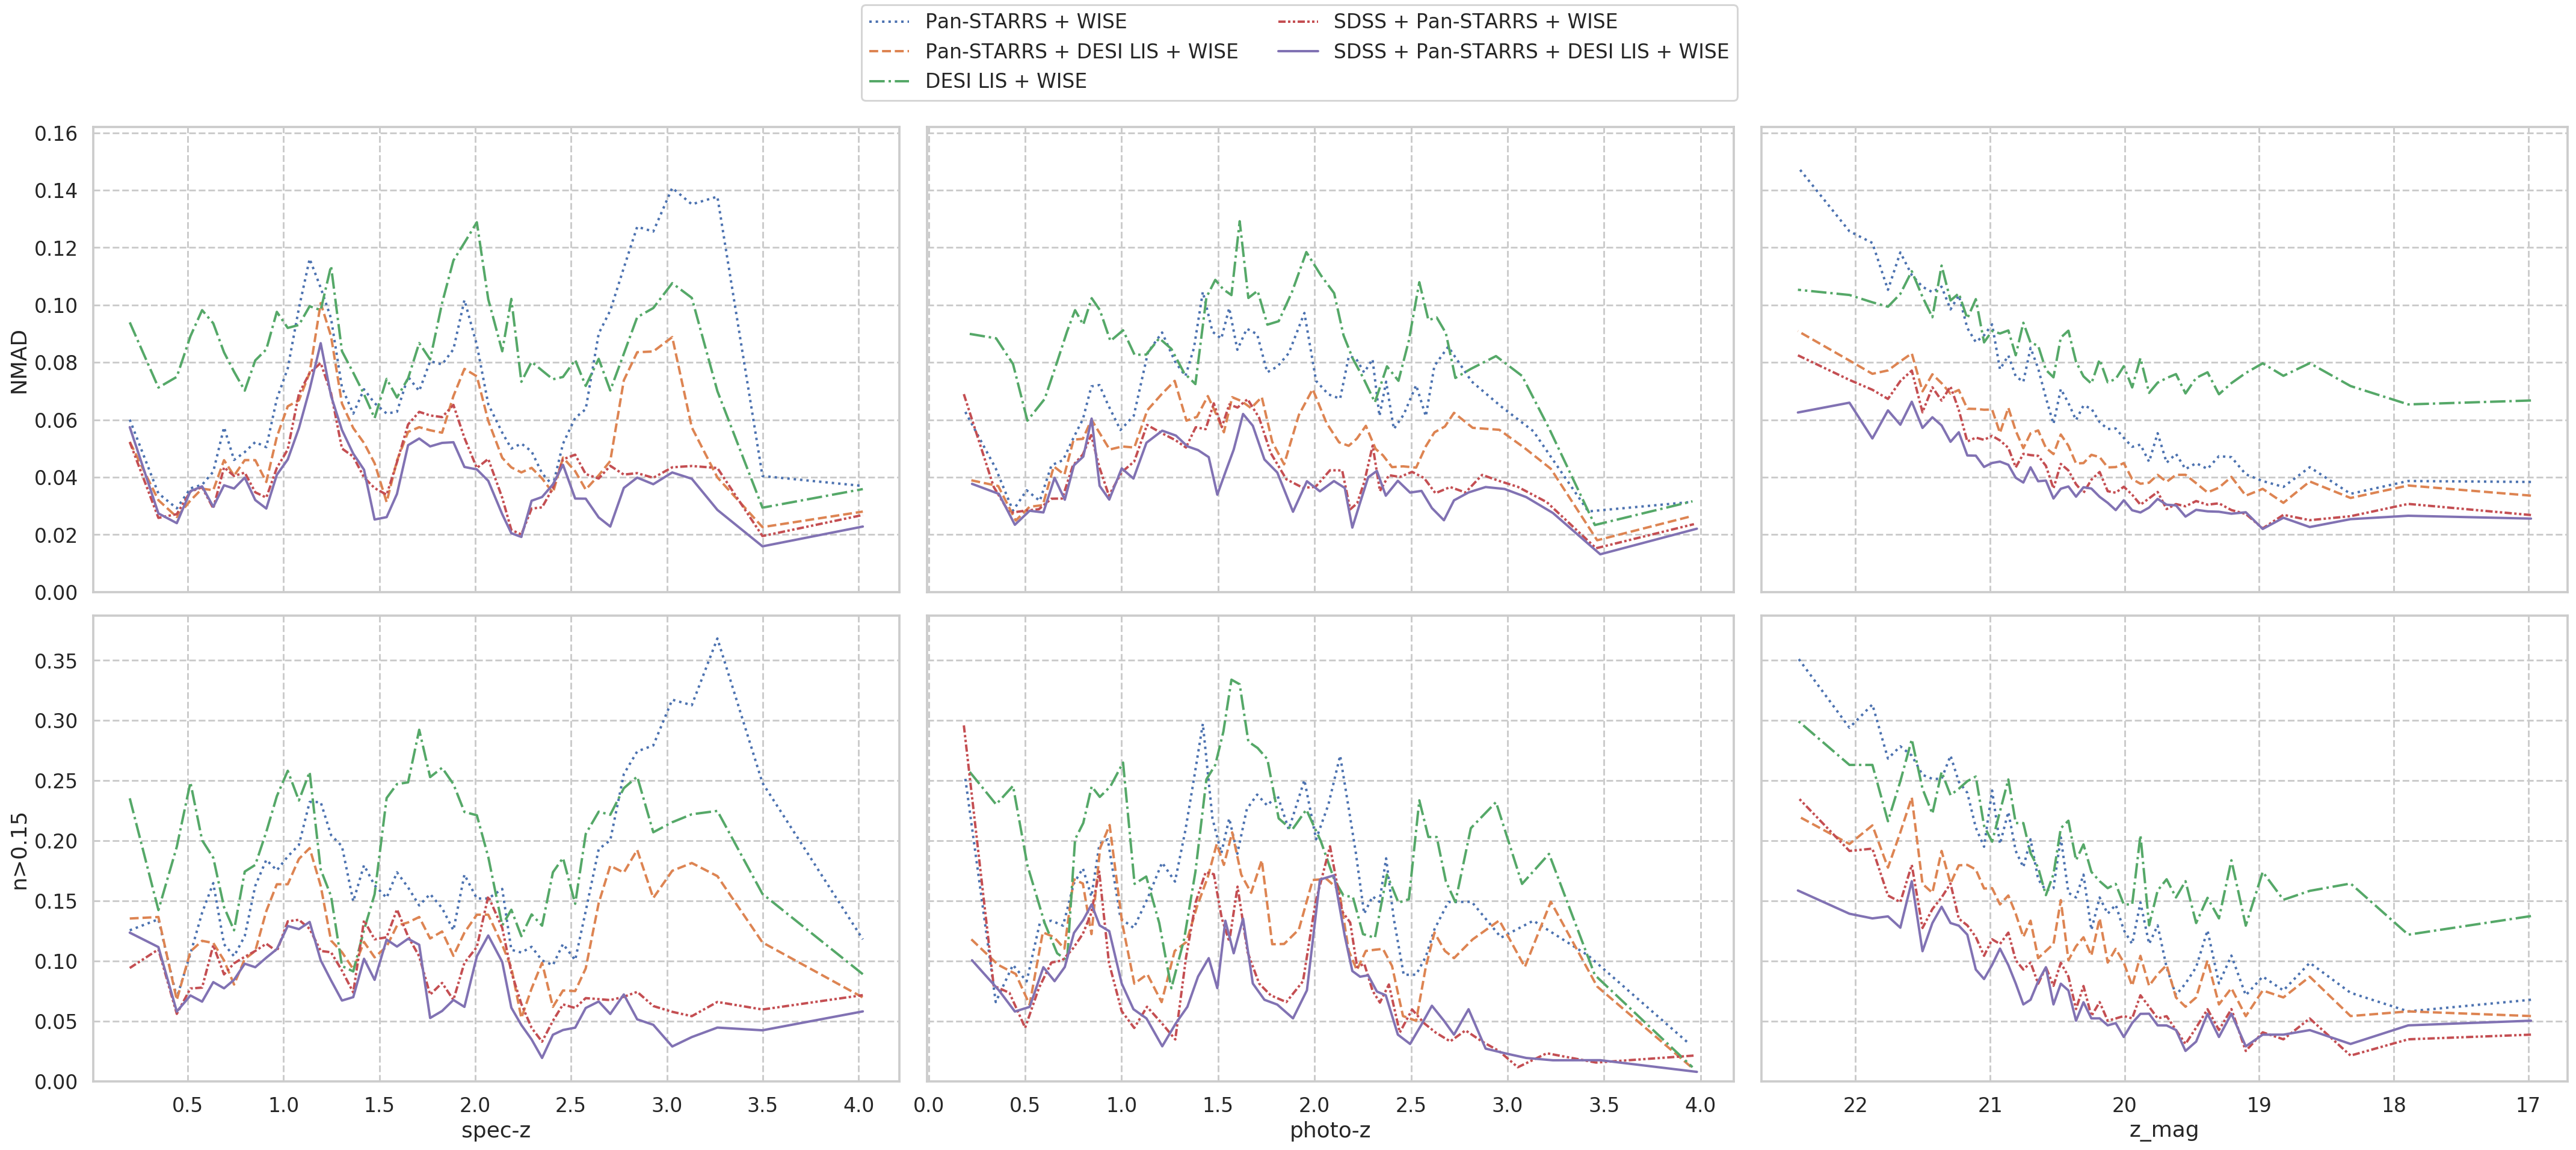
\includegraphics[width=0.9\linewidth]{images/metrics-dr16q-ab-mini.png}
    \caption{Plots of NMAD \eqref{eq:nmad} (upper line of plots) and the fraction of catastrophic outliers \eqref{eq:n015} (lower line of plots) metrics as a function of (from left to right) spectral redshift value, photometric redshift prediction value, and stellar magnitude in the filter z) on DR16q quasars test sample. The solid line shows model \ref{model:spdw}, the dot line shows model \ref{model:pw}, the dashed line shows model \ref{model:pdw}, the dash-dot line shows model \ref{model:dw}, and dash-dot-dot line shows model \ref{model:spw}.}
    \label{fig:metrics-dr16q}
\end{figure*}

\begin{table*}
	\begin{tabular}{llrrrrrrrrr}
            \hline
                              &                  & \multicolumn{3}{l}{Stripe82x-A17 sample} & \multicolumn{3}{l}{Quasars of DR16q} & \multicolumn{3}{l}{Cross-Validation} \\
                              &                  &               $NMAD$ &        $n>0.15$ &  $C_{68} - 0.68$ &           $NMAD$ &        $n>0.15$ &  $C_{68} - 0.68$ &           $NMAD$ &        $n>0.15$ &  $C_{68} - 0.68$ \\
            subsample & model &                      &                 &                  &                  &                 &                  &                  &                 &                  \\

\hline
            All objects       & \ref{model:pw} &                0.056 &           0.149 &            0.023 &            0.063 &           0.165 &            0.031 &            0.046 &           0.109 &            0.052 \\
                              & \ref{model:pdw} &                0.046 &           0.113 &            0.075 &            0.049 &            0.12 &            0.068 &            0.037 &           0.085 &            0.072 \\
                              & \ref{model:dw} &                0.074 &           0.177 &  \textbf{-0.003} &            0.083 &            0.19 &  \textbf{-0.005} &            0.058 &           0.143 &  \textbf{-0.008} \\
                              & \ref{model:spw} &                 0.04 &           0.105 &            0.089 &             0.04 &           0.088 &            0.082 &            0.031 &           0.054 &            0.084 \\
                              & \ref{model:spdw} &       \textbf{0.034} &  \textbf{0.089} &            0.104 &   \textbf{0.037} &  \textbf{0.076} &            0.093 &   \textbf{0.028} &  \textbf{0.048} &            0.093 \\
\hline
\hline
            $z_{spec} < 0.5$ & \ref{model:pw} &                0.038 &  \textbf{0.083} &   \textbf{0.003} &            0.038 &           0.113 &   \textbf{0.028} &             0.02 &           0.031 &            0.045 \\
                              & \ref{model:pdw} &                0.031 &           0.086 &             0.04 &            0.033 &           0.112 &            0.044 &            0.016 &           0.027 &            0.072 \\
                              & \ref{model:dw} &                0.048 &           0.111 &            0.035 &            0.077 &           0.197 &           -0.056 &            0.019 &           0.045 &  \textbf{-0.004} \\
                              & \ref{model:spw} &                0.032 &  \textbf{0.083} &            0.044 &            0.032 &  \textbf{0.085} &            0.063 &            0.018 &           0.026 &            0.076 \\
                              & \ref{model:spdw} &        \textbf{0.03} &           0.084 &            0.062 &   \textbf{0.031} &           0.097 &            0.056 &   \textbf{0.015} &  \textbf{0.025} &            0.094 \\
\hline
            $0.5 \leq z_{spec} < 1$ & \ref{model:pw} &                0.053 &           0.147 &             0.03 &            0.048 &           0.139 &            0.061 &            0.037 &           0.088 &             0.06 \\
                              & \ref{model:pdw} &                0.047 &           0.138 &            0.072 &            0.042 &           0.112 &            0.084 &             0.03 &           0.078 &             0.08 \\
                              & \ref{model:dw} &                0.081 &           0.204 &  \textbf{-0.011} &            0.085 &           0.186 &  \textbf{-0.023} &            0.049 &           0.126 &  \textbf{-0.013} \\
                              & \ref{model:spw} &                0.043 &           0.111 &            0.109 &            0.037 &           0.097 &            0.106 &             0.03 &            0.06 &            0.099 \\
                              & \ref{model:spdw} &       \textbf{0.038} &  \textbf{0.106} &            0.122 &   \textbf{0.035} &  \textbf{0.089} &            0.124 &   \textbf{0.026} &  \textbf{0.058} &            0.111 \\
\hline
            $1 \leq z_{spec} < 1.5$ & \ref{model:pw} &                0.079 &           0.173 &            0.025 &            0.083 &           0.195 &            0.031 &            0.069 &           0.142 &            0.051 \\
                              & \ref{model:pdw} &                0.061 &           0.109 &            0.074 &             0.07 &           0.146 &            0.066 &            0.059 &           0.099 &            0.074 \\
                              & \ref{model:dw} &                0.083 &           0.143 &    \textbf{0.01} &            0.088 &           0.177 &   \textbf{0.005} &            0.078 &           0.134 &   \textbf{0.019} \\
                              & \ref{model:spw} &                0.053 &           0.108 &            0.097 &            0.058 &           0.113 &             0.11 &            0.046 &            0.07 &            0.099 \\
                              & \ref{model:spdw} &       \textbf{0.048} &  \textbf{0.088} &            0.122 &   \textbf{0.057} &    \textbf{0.1} &            0.107 &   \textbf{0.043} &   \textbf{0.06} &            0.105 \\
\hline
            $1.5 \leq z_{spec} < 2$ & \ref{model:pw} &                0.075 &           0.158 &            0.075 &            0.076 &           0.157 &            0.088 &            0.069 &           0.142 &            0.061 \\
                              & \ref{model:pdw} &                0.043 &           0.102 &            0.127 &            0.056 &           0.128 &            0.088 &            0.051 &           0.109 &            0.077 \\
                              & \ref{model:dw} &                0.078 &           0.253 &  \textbf{-0.029} &            0.093 &           0.256 &  \textbf{-0.009} &            0.089 &           0.238 &  \textbf{-0.042} \\
                              & \ref{model:spw} &                 0.04 &           0.096 &            0.163 &            0.053 &           0.103 &            0.115 &            0.043 &           0.073 &            0.101 \\
                              & \ref{model:spdw} &       \textbf{0.031} &  \textbf{0.065} &            0.144 &   \textbf{0.044} &  \textbf{0.093} &             0.12 &   \textbf{0.038} &  \textbf{0.061} &            0.105 \\
\hline
            $2 \leq z_{spec}$ & \ref{model:pw} &                0.071 &           0.222 &  \textbf{-0.018} &            0.063 &           0.173 &  \textbf{-0.001} &            0.058 &           0.132 &            0.046 \\
                              & \ref{model:pdw} &                0.046 &           0.133 &            0.089 &            0.046 &           0.111 &            0.059 &            0.047 &           0.101 &            0.064 \\
                              & \ref{model:dw} &                0.091 &           0.206 &           -0.043 &            0.078 &           0.172 &            0.005 &             0.08 &           0.164 &  \textbf{-0.002} \\
                              & \ref{model:spw} &                0.039 &            0.14 &             0.03 &            0.035 &            0.07 &            0.053 &            0.033 &           0.048 &            0.064 \\
                              & \ref{model:spdw} &       \textbf{0.029} &  \textbf{0.098} &            0.072 &   \textbf{0.031} &  \textbf{0.055} &            0.072 &    \textbf{0.03} &  \textbf{0.043} &            0.072 \\
\hline
\hline
            $z_{mag} < 19$ & \ref{model:pw} &                0.037 &           0.046 &   \textbf{0.015} &            0.039 &           0.077 &            0.053 &            0.025 &           0.033 &            0.059 \\
                                   & \ref{model:pdw} &                0.027 &            0.04 &            0.043 &            0.034 &           0.068 &            0.066 &             0.02 &           0.029 &            0.077 \\
                                   & \ref{model:dw} &                0.038 &            0.08 &            0.036 &            0.071 &           0.152 &  \textbf{-0.012} &            0.026 &            0.06 &  \textbf{-0.006} \\
                                   & \ref{model:spw} &       \textbf{0.024} &           0.038 &            0.062 &            0.026 &  \textbf{0.035} &            0.102 &            0.019 &           0.018 &            0.092 \\
                                   & \ref{model:spdw} &       \textbf{0.024} &  \textbf{0.029} &            0.081 &   \textbf{0.025} &            0.04 &            0.096 &   \textbf{0.017} &  \textbf{0.017} &            0.104 \\
\hline
            $19 \leq z_{mag} < 20$ & \ref{model:pw} &                0.043 &           0.076 &            0.075 &            0.046 &           0.098 &            0.065 &            0.043 &           0.079 &            0.059 \\
                                   & \ref{model:pdw} &                0.036 &           0.065 &            0.114 &            0.038 &           0.075 &            0.082 &            0.035 &           0.064 &            0.076 \\
                                   & \ref{model:dw} &                0.071 &            0.11 &   \textbf{0.008} &            0.074 &           0.154 &  \textbf{-0.004} &            0.058 &           0.124 &  \textbf{-0.006} \\
                                   & \ref{model:spw} &                0.031 &           0.045 &            0.115 &             0.03 &            0.05 &            0.095 &            0.029 &           0.037 &             0.09 \\
                                   & \ref{model:spdw} &       \textbf{0.028} &  \textbf{0.041} &            0.131 &   \textbf{0.028} &  \textbf{0.044} &            0.099 &   \textbf{0.027} &  \textbf{0.035} &            0.097 \\
\hline
            $20 \leq z_{mag} < 20.5$ & \ref{model:pw} &                0.064 &           0.137 &            0.027 &            0.058 &           0.145 &            0.031 &            0.058 &           0.129 &            0.052 \\
                                   & \ref{model:pdw} &                0.046 &           0.105 &            0.107 &            0.045 &           0.105 &            0.069 &            0.048 &             0.1 &            0.071 \\
                                   & \ref{model:dw} &                0.075 &           0.165 &   \textbf{0.014} &            0.079 &           0.172 &   \textbf{0.007} &            0.081 &           0.174 &  \textbf{-0.007} \\
                                   & \ref{model:spw} &                0.041 &           0.087 &            0.105 &            0.037 &           0.065 &            0.083 &            0.037 &           0.059 &            0.087 \\
                                   & \ref{model:spdw} &       \textbf{0.033} &  \textbf{0.074} &            0.107 &   \textbf{0.033} &  \textbf{0.056} &            0.101 &   \textbf{0.034} &  \textbf{0.054} &            0.094 \\
\hline
            $20.5 \leq z_{mag} < 21$ & \ref{model:pw} &                0.076 &           0.199 &           -0.009 &            0.072 &           0.183 &            0.024 &            0.072 &           0.168 &             0.04 \\
                                   & \ref{model:pdw} &                0.056 &           0.121 &            0.078 &            0.054 &           0.127 &            0.077 &            0.057 &           0.128 &            0.063 \\
                                   & \ref{model:dw} &                0.088 &           0.219 &   \textbf{0.006} &            0.084 &           0.198 &   \textbf{0.004} &            0.089 &           0.206 &  \textbf{-0.011} \\
                                   & \ref{model:spw} &                0.054 &           0.126 &            0.076 &            0.046 &           0.099 &            0.067 &            0.044 &           0.083 &            0.072 \\
                                   & \ref{model:spdw} &       \textbf{0.044} &  \textbf{0.106} &            0.105 &   \textbf{0.039} &  \textbf{0.082} &             0.09 &    \textbf{0.04} &  \textbf{0.073} &            0.081 \\
\hline
            $21 \leq z_{mag} < 23$ & \ref{model:pw} &                0.119 &           0.319 &  \textbf{-0.011} &            0.102 &           0.258 &  \textbf{-0.003} &            0.088 &           0.213 &            0.037 \\
                                   & \ref{model:pdw} &                0.082 &           0.245 &            0.035 &            0.071 &           0.179 &            0.051 &            0.066 &           0.157 &            0.065 \\
                                   & \ref{model:dw} &                0.118 &           0.325 &           -0.073 &            0.098 &           0.236 &           -0.016 &            0.096 &           0.229 &  \textbf{-0.011} \\
                                   & \ref{model:spw} &                0.082 &           0.252 &            0.085 &            0.064 &           0.151 &            0.072 &            0.054 &           0.111 &            0.069 \\
                                   & \ref{model:spdw} &       \textbf{0.063} &   \textbf{0.21} &            0.095 &   \textbf{0.054} &  \textbf{0.124} &            0.085 &   \textbf{0.048} &  \textbf{0.094} &             0.08 \\
\hline
            \hline
            \end{tabular}
            \caption{Prediction metrics for models \ref{model:pw} -- \ref{model:spdw}. The first column shows the subsample of the whole sample, the second column the model number. The next three columns -- NMAD \eqref{eq:nmad}, catastrophic outliers fraction \eqref{eq:n015}, and 68\% confidence interval calibration \eqref{eq:c68} metrics on the Stripe82X X-ray object test sample, the second three columns -- on the SDSS DR16q quasar test sample, and the last three columns -- on cross-validation.}
\end{table*}

\begin{table*}
	\begin{tabular}{llllllllll}
            \hline
            {} & \multicolumn{3}{l}{$FSoft < 1e-14$ (951 objects)} & \multicolumn{3}{l}{$FSoft < 4e-14$ (2016 objects)} & \multicolumn{3}{l}{All (2223 objects)} \\
            {} &                        $NMAD$ &        $n>0.15$ & $C_{68} - 0.68$ &                         $NMAD$ &        $n>0.15$ &  $C_{68} - 0.68$ &                       $NMAD$ &        $n>0.15$ &  $C_{68} - 0.68$ \\
            Model            &                               &                 &                 &                                &                 &                  &                              &                 &                  \\
            \hline
            \ref{model:pw}   &                         0.068 &           0.188 &           0.016 &                          0.058 &           0.154 &            0.026 &                        0.056 &           0.148 &            0.026 \\
            \ref{model:pdw}  &                         0.049 &           0.127 &           0.084 &                          0.047 &           0.113 &             0.08 &                        0.045 &           0.108 &             0.08 \\
            \ref{model:dw}   &                         0.073 &           0.196 &  \textbf{0.005} &                          0.073 &           0.176 &  \textbf{-0.006} &                        0.073 &           0.172 &  \textbf{-0.011} \\
            \ref{model:spw}  &                         0.048 &           0.138 &           0.079 &                          0.042 &            0.11 &            0.091 &                         0.04 &           0.105 &            0.092 \\
            \ref{model:spdw} &                \textbf{0.038} &  \textbf{0.107} &             0.1 &                 \textbf{0.035} &  \textbf{0.092} &            0.109 &               \textbf{0.033} &  \textbf{0.088} &             0.11 \\
            Template Model   &                         0.061 &           0.161 &          -0.284 &                          0.064 &            0.17 &           -0.324 &                        0.064 &           0.175 &           -0.339 \\
            NN Model         &                         0.063 &           0.145 &          -0.199 &                          0.065 &           0.153 &           -0.243 &                        0.065 &           0.159 &           -0.256 \\
            \hline
            \end{tabular}
            \caption{Prediction metrics for models \ref{model:pw} -- \ref{model:spdw}, template model (Ananna, 2017) and neural network model (Brescia, 2019) on Stripe82X X-ray test sample. The first column shows model, the next three columns -- NMAD \eqref{eq:nmad}, catastrophic outliers fraction \eqref{eq:n015}, and 68\% confidence interval calibration \eqref{eq:c68} metrics for objects with $FSoft < 1e-14$, the second three columns -- for objects with $FSoft < 4e-14$, and the last three columns -- for the entire sample.}
\end{table*}

\subsection{PDZ reliability}

\begin{figure*}
    \centering
    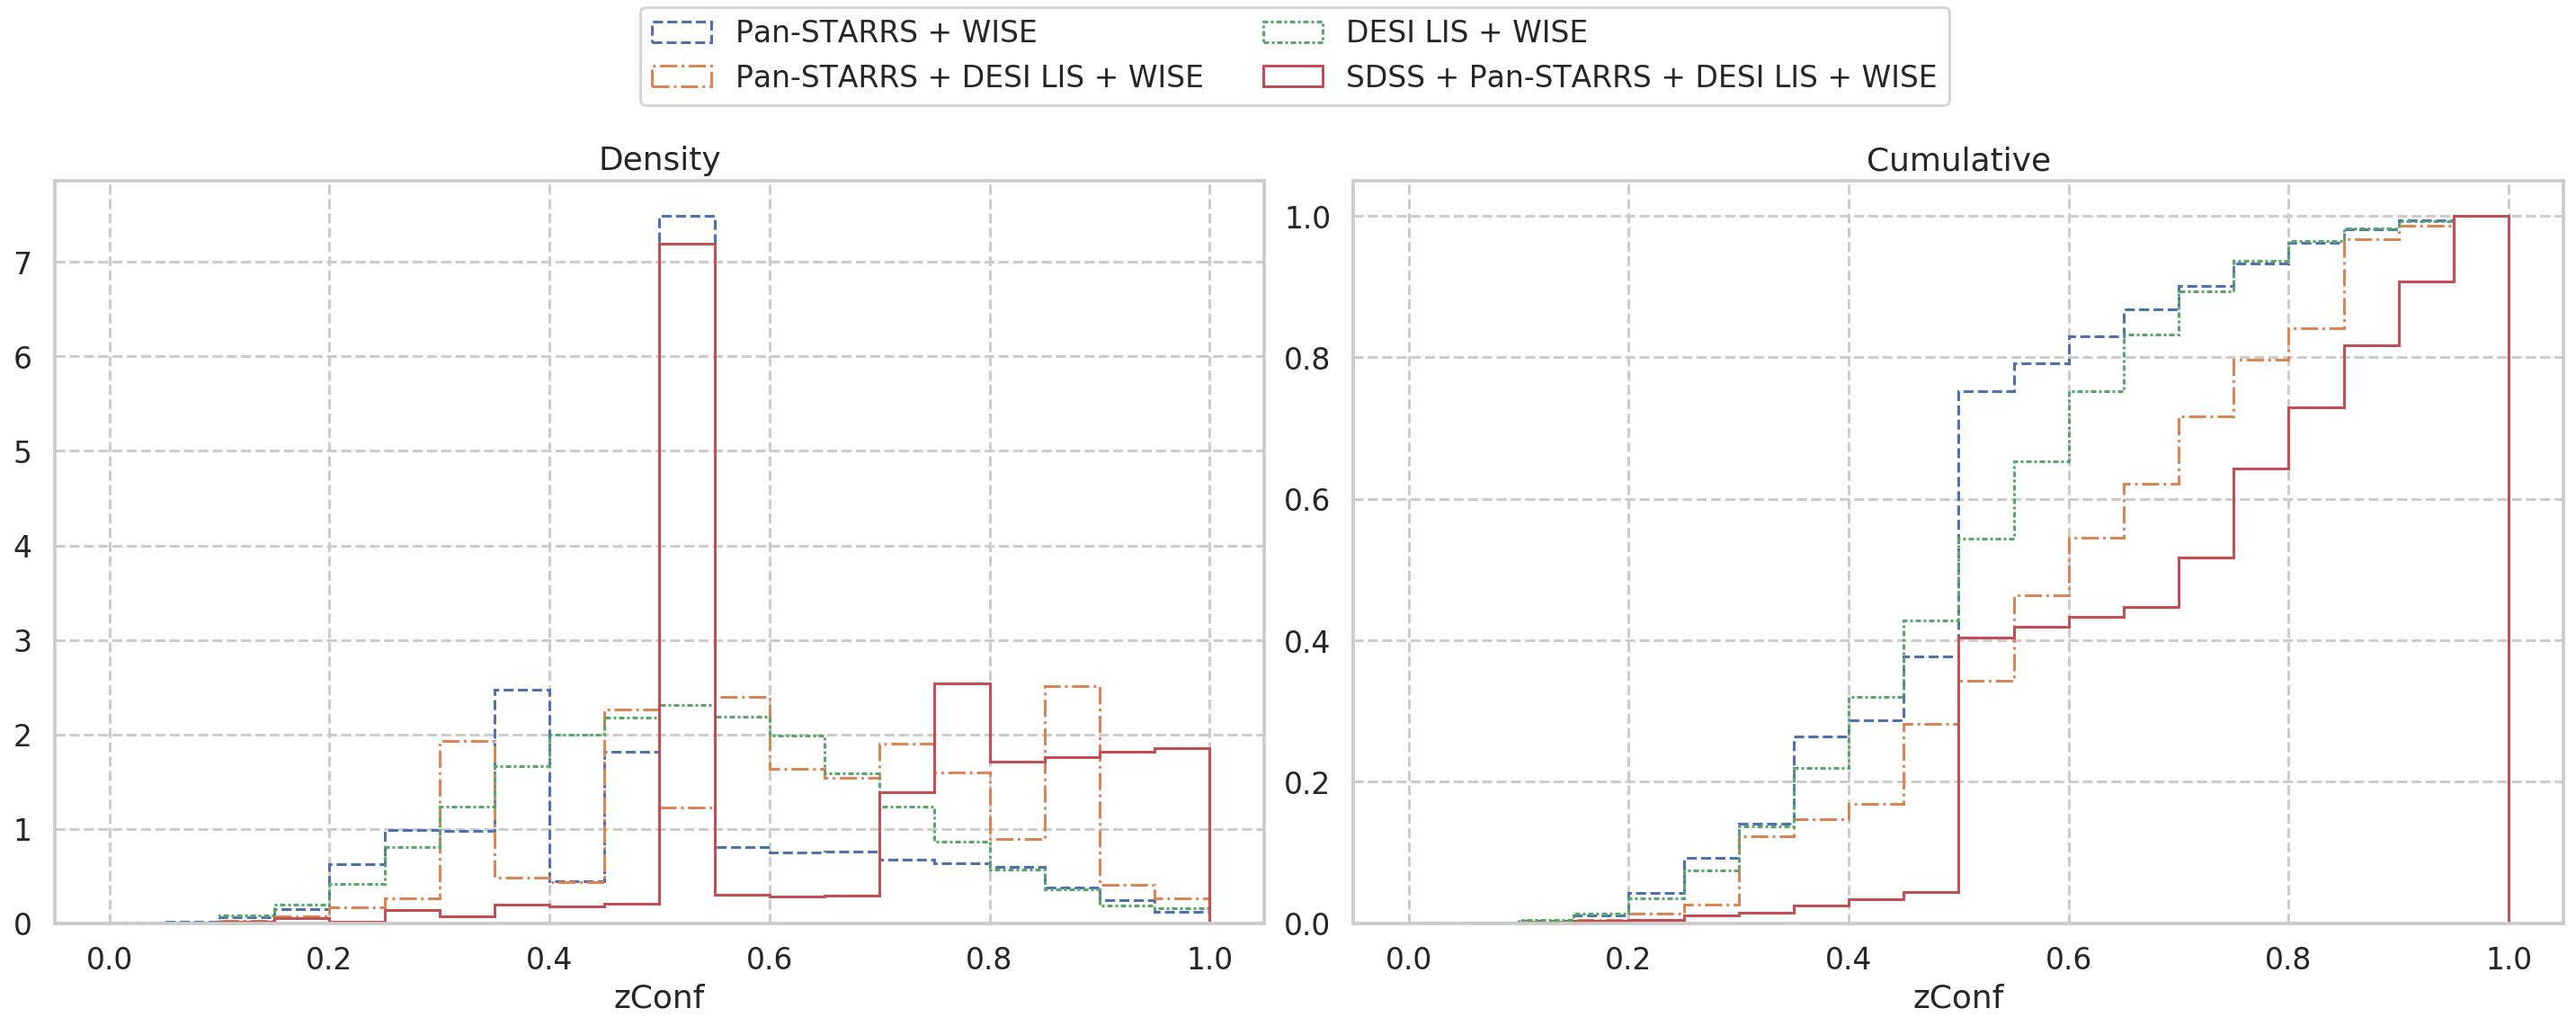
\includegraphics[width=0.9\linewidth]{images/zconf-cal-dr16q.png}
    \caption{zConf distribution on DR16q test sample}
    \label{fig:zconf-cal-dr16q}
\end{figure*}

\begin{figure*}
    \centering
    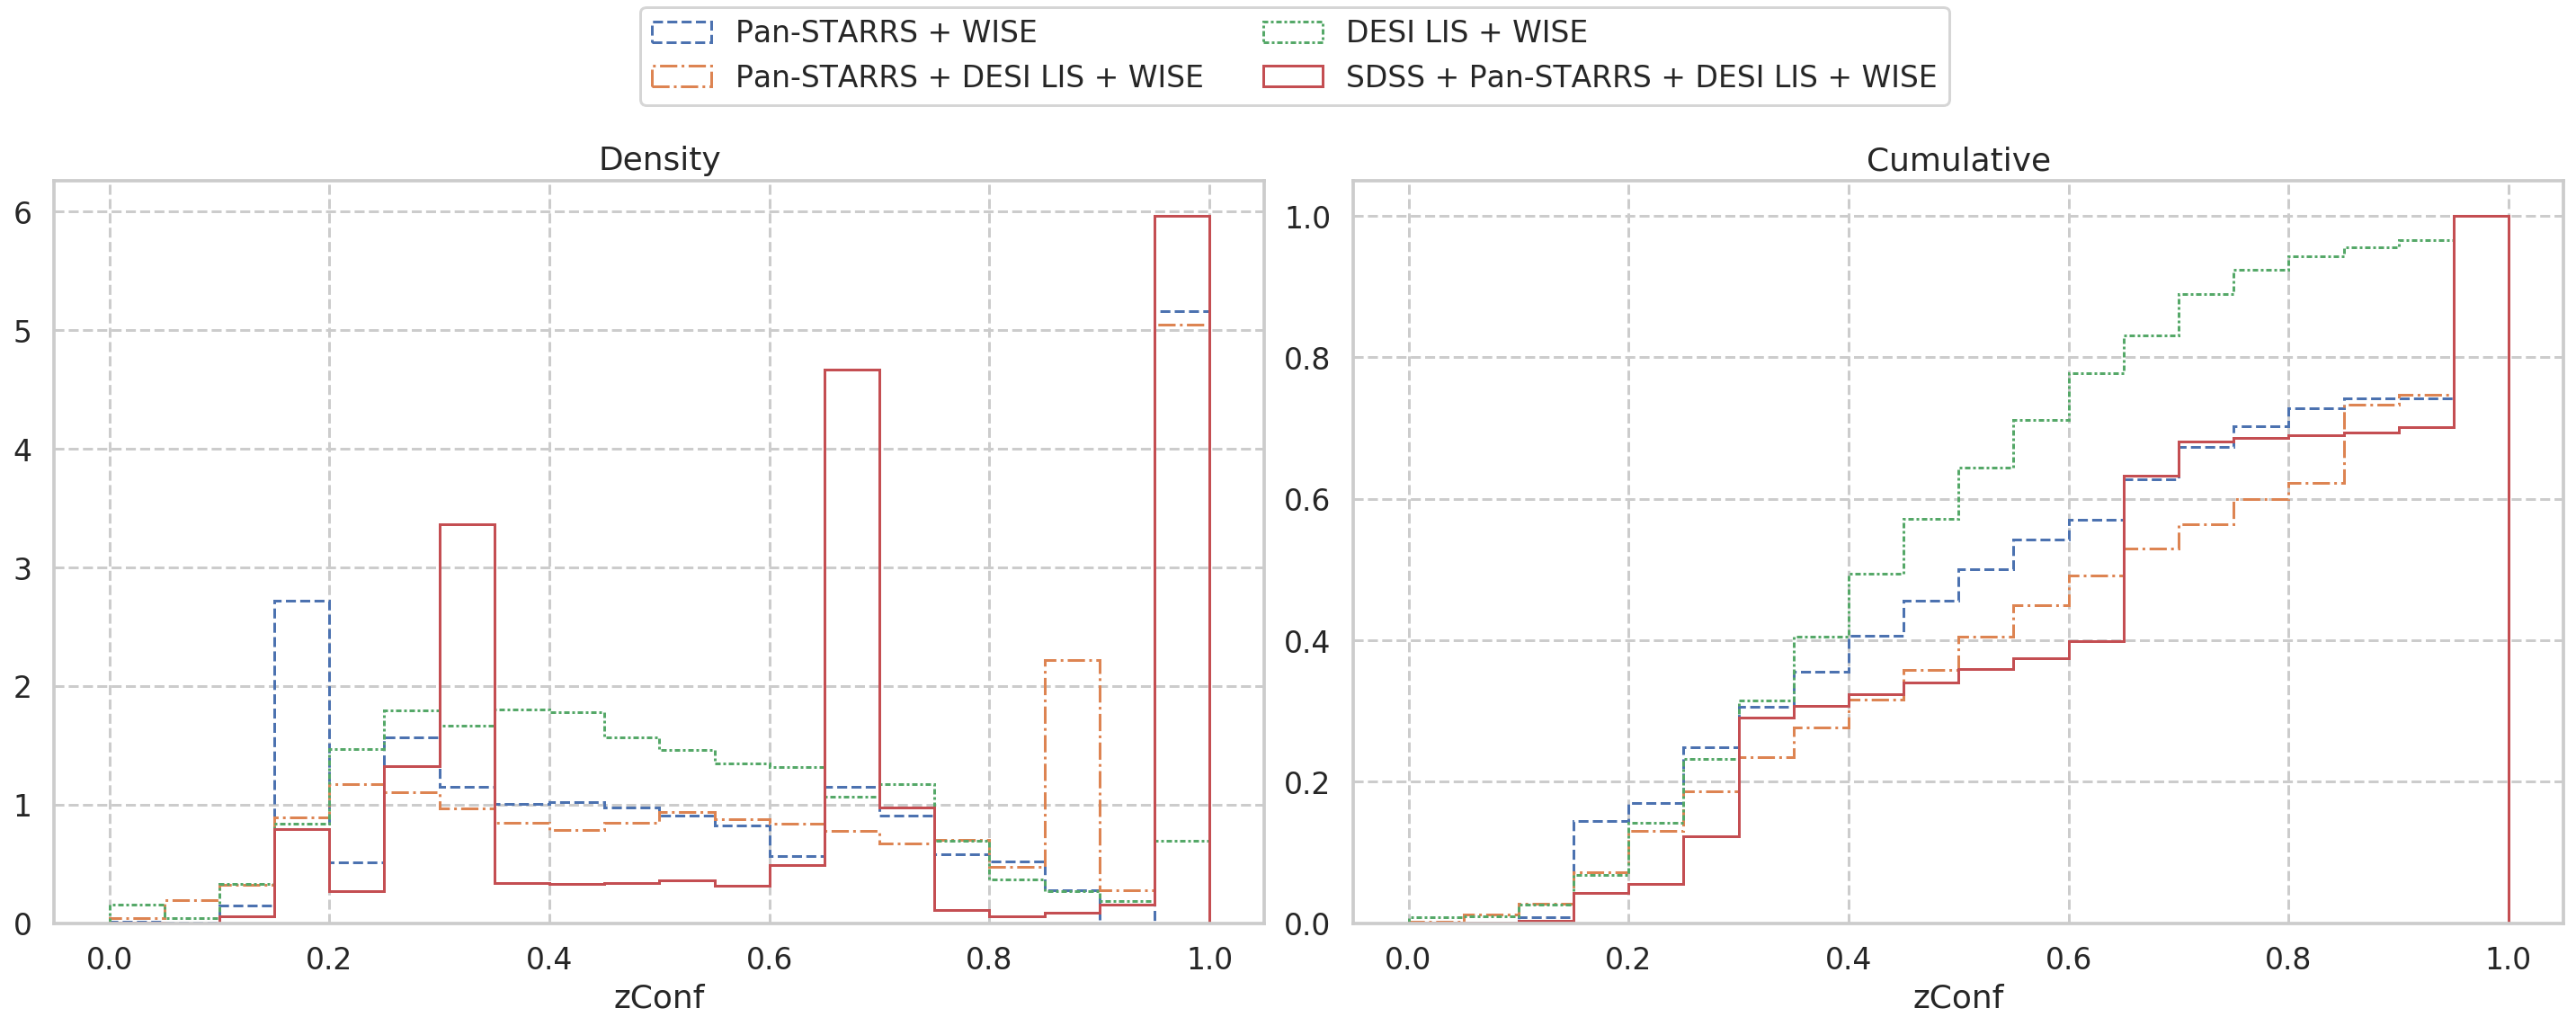
\includegraphics[width=0.9\linewidth]{images/zconf-cal-stripe82X.png}
    \caption{zConf distribution on Stripe82X test sample}
    \label{fig:zconf-cal-stripe82X}
\end{figure*}

% ===============================================================================
% ===============================================================================
% ===============================================================================

\section{Conclusion}

% В рамках работы было построено множество моделей photo-z на основе различных признаков, которые строятся по данным трех современных фотометрических обзоров~--- SDSS, Pan-STARRS1 и DESI Legacy Imaging Survey. Обучающая выборка состоит из $\sim$580000 оптических квазаров и галактик и сбалансирована, чтобы аппроксимировать распределение рентгеновских объектов. Разметка взята из спектрального каталога оптических объектов SDSS.

% На тестовой выборке рентгеновских объектов поля Stripe82X \cite{bib:ananna}, за счет использования данных всех трех вышеупомянутых обзоров, была достигнута точность по метрикам $NMAD$ и доля выбросов $n_{>0.15}$ значительно выше (почти в 2 раза), чем точность лучших моделей известных в литературе (SOTA), что является основным результатом работы. Для лучшей модели / шаблонной модели \cite{bib:ananna} / нейросетевой модели \cite{bib:brescia} на выборке Stripe82X получены значения метрик $NMAD$ = 0.034 / 0.065 / 0.066 и $n_{>0.15}$ = 0.088 / 0.170 / 0.156, соответственно.

The proposed photo-z models based on Random Forests show accuracy (up to 2 times) better than current SOTA results in the literature (on Stripe82X field). The main accuracy improvement comes from using a large training sample ($\sim$600k objects) with features from modern wide photometric surveys. First optical spectroscopic observations of eRosita sources show that the proposed photo-z models are effective in the ongoing search for distant X-ray quasars (see e.g. \citep{2020MNRAS.497.1842M,2020AstL...46..149K,2020AstL...46..429D}).

The presented photo-z models are integrated into the SRGz system designed to construct a three-dimensional map of X-ray sources on the Eastern Galactic Hemisphere of the SRG/eRosita All-Sky survey. The SRGz system is developed in the science working group of RU eROSITA consortium on X-ray source detection, identification, and eROSITA source catalog in the High Energy Astrophysics Department at Space Research Institute of the Russian Academy of Sciences.

% ===============================================================================
% ===============================================================================
% ===============================================================================

\section{Discussion}

Провалы в точности по zspec. Переход на ансамбли нейронных сетей. Источник данных о поглощении на всем небе?

\section*{Acknowledgments}
..

% bibliograpgy 
\bibliographystyle{mnras}
\bibliography{main}

\appendix

\section{Advanced metrics charts}

\begin{landscape}
\begin{figure}
    \centering
    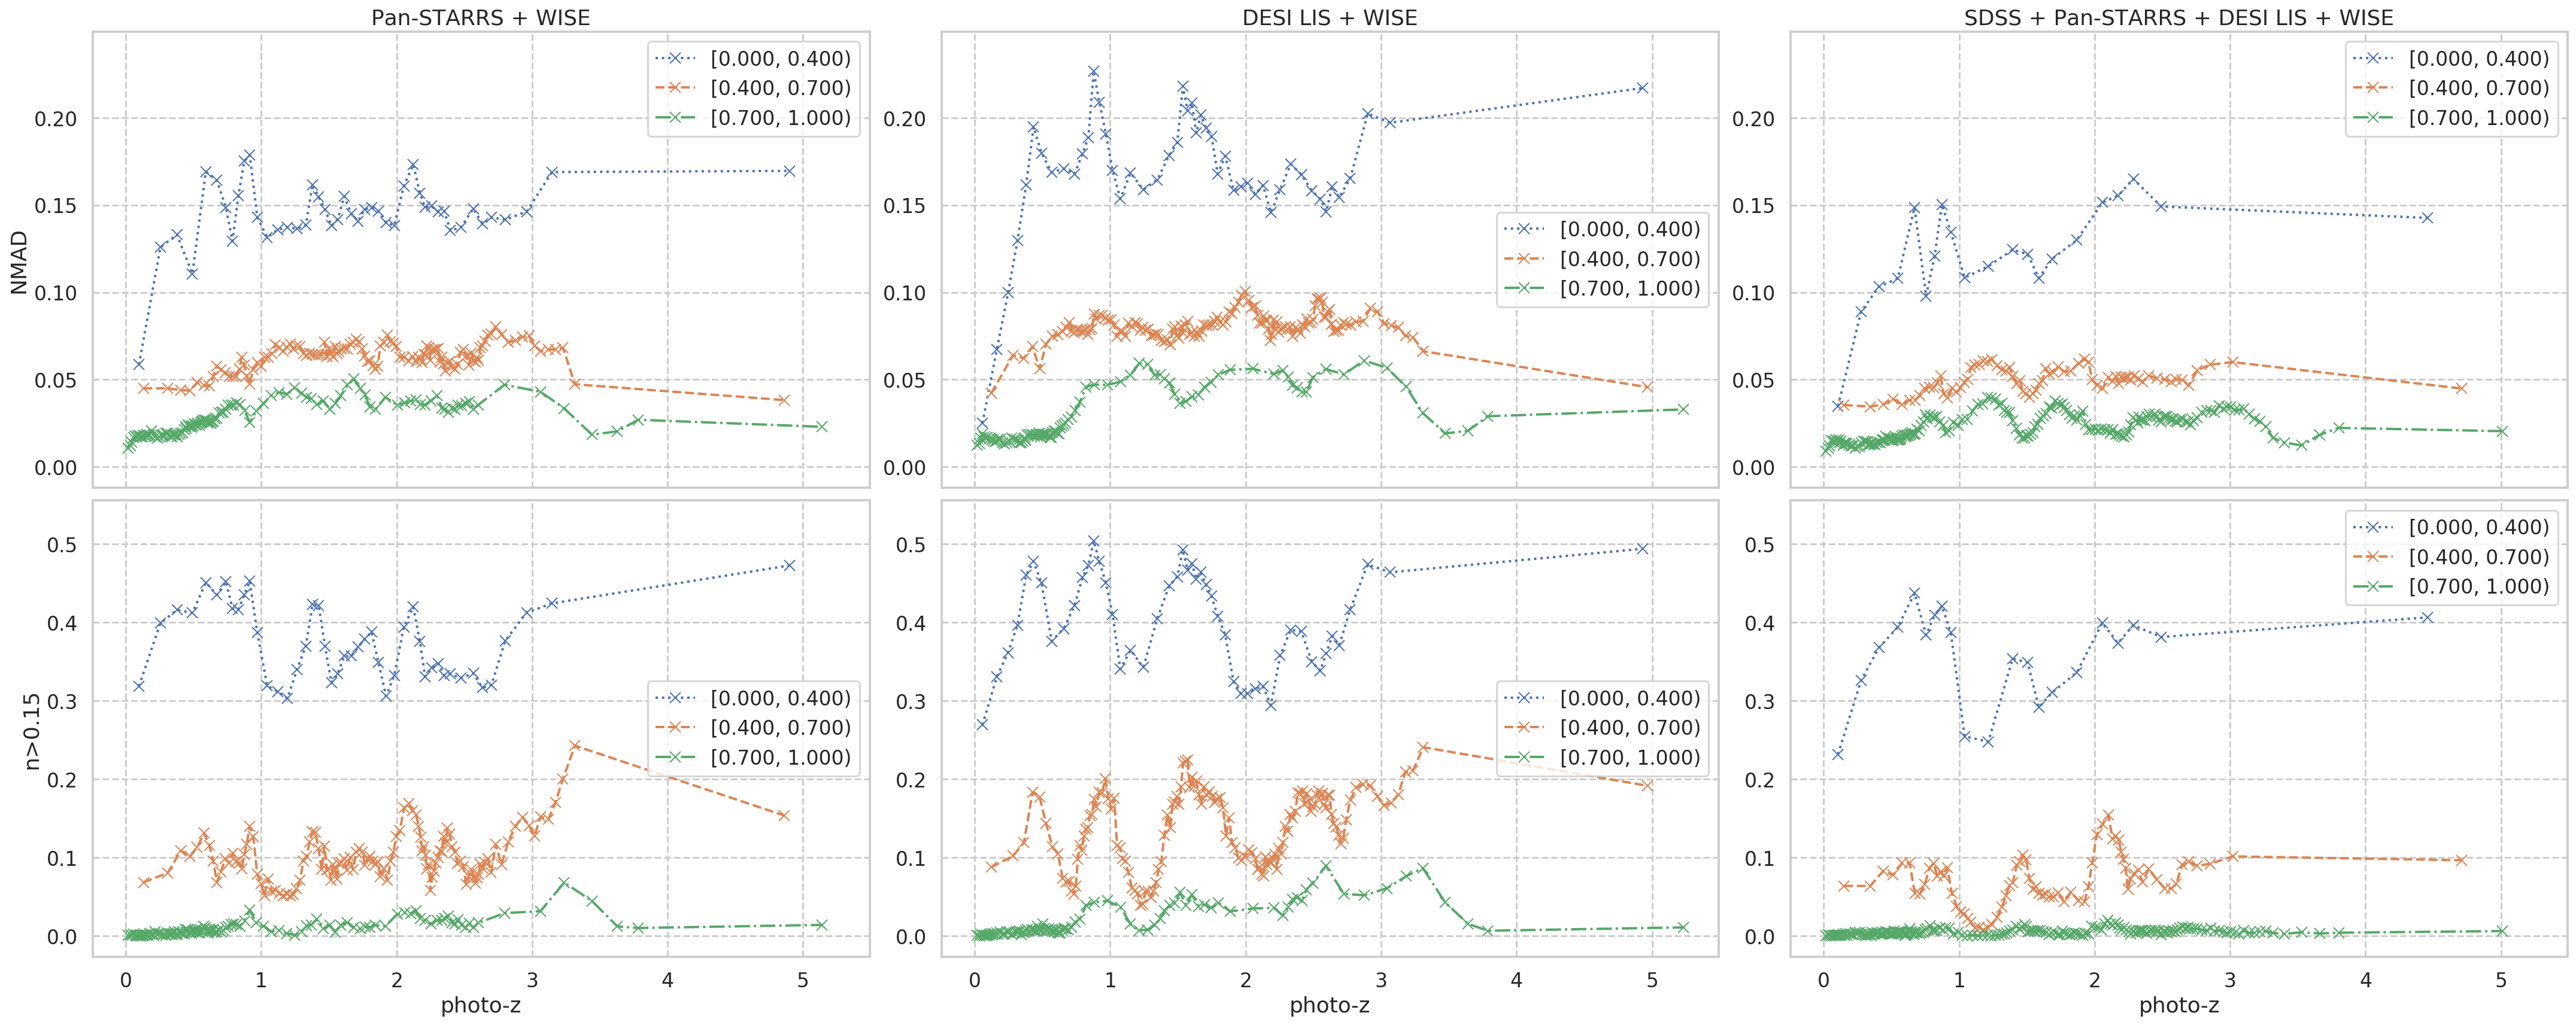
\includegraphics[width=25cm]{images/metrics-adv-photoz-x-zconf-cv2.png}
    \caption{Метрики в зависимости от photo-z для разных порогов по zConf на кросс-валидации}
    \label{fig:my_label}
\end{figure}
\end{landscape}


\begin{landscape}
\begin{figure}
    \centering
    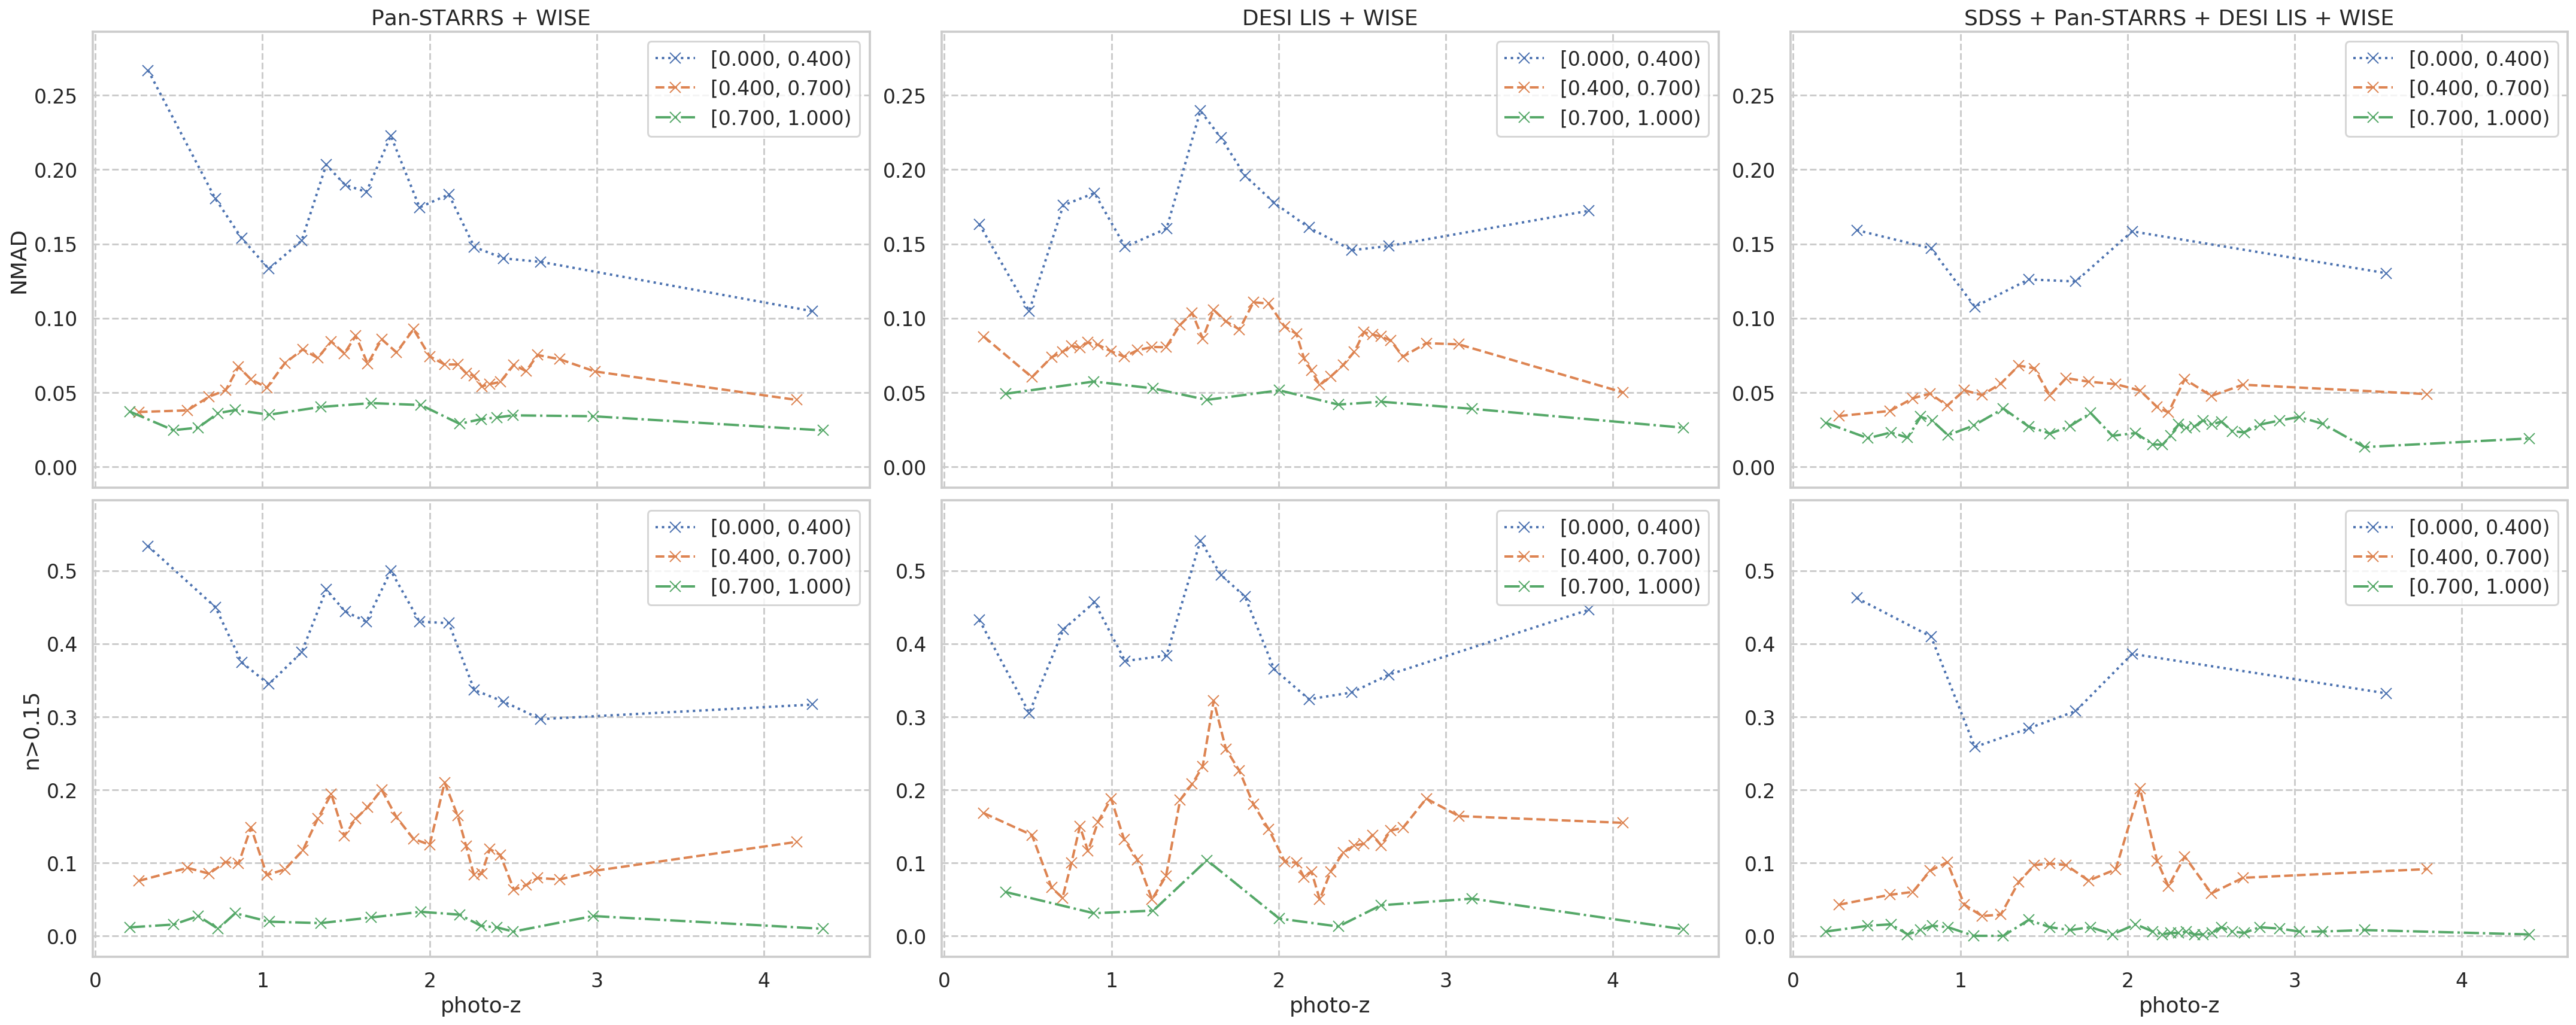
\includegraphics[width=0.9\linewidth]{images/metrics-adv-photoz-x-zconf-dr16q.png}
    \caption{Метрики в зависимости от photo-z для разных порогов по zConf на DR16q}
    \label{fig:my_label}
\end{figure}
\end{landscape}


\begin{landscape}
\begin{figure}
    \centering
    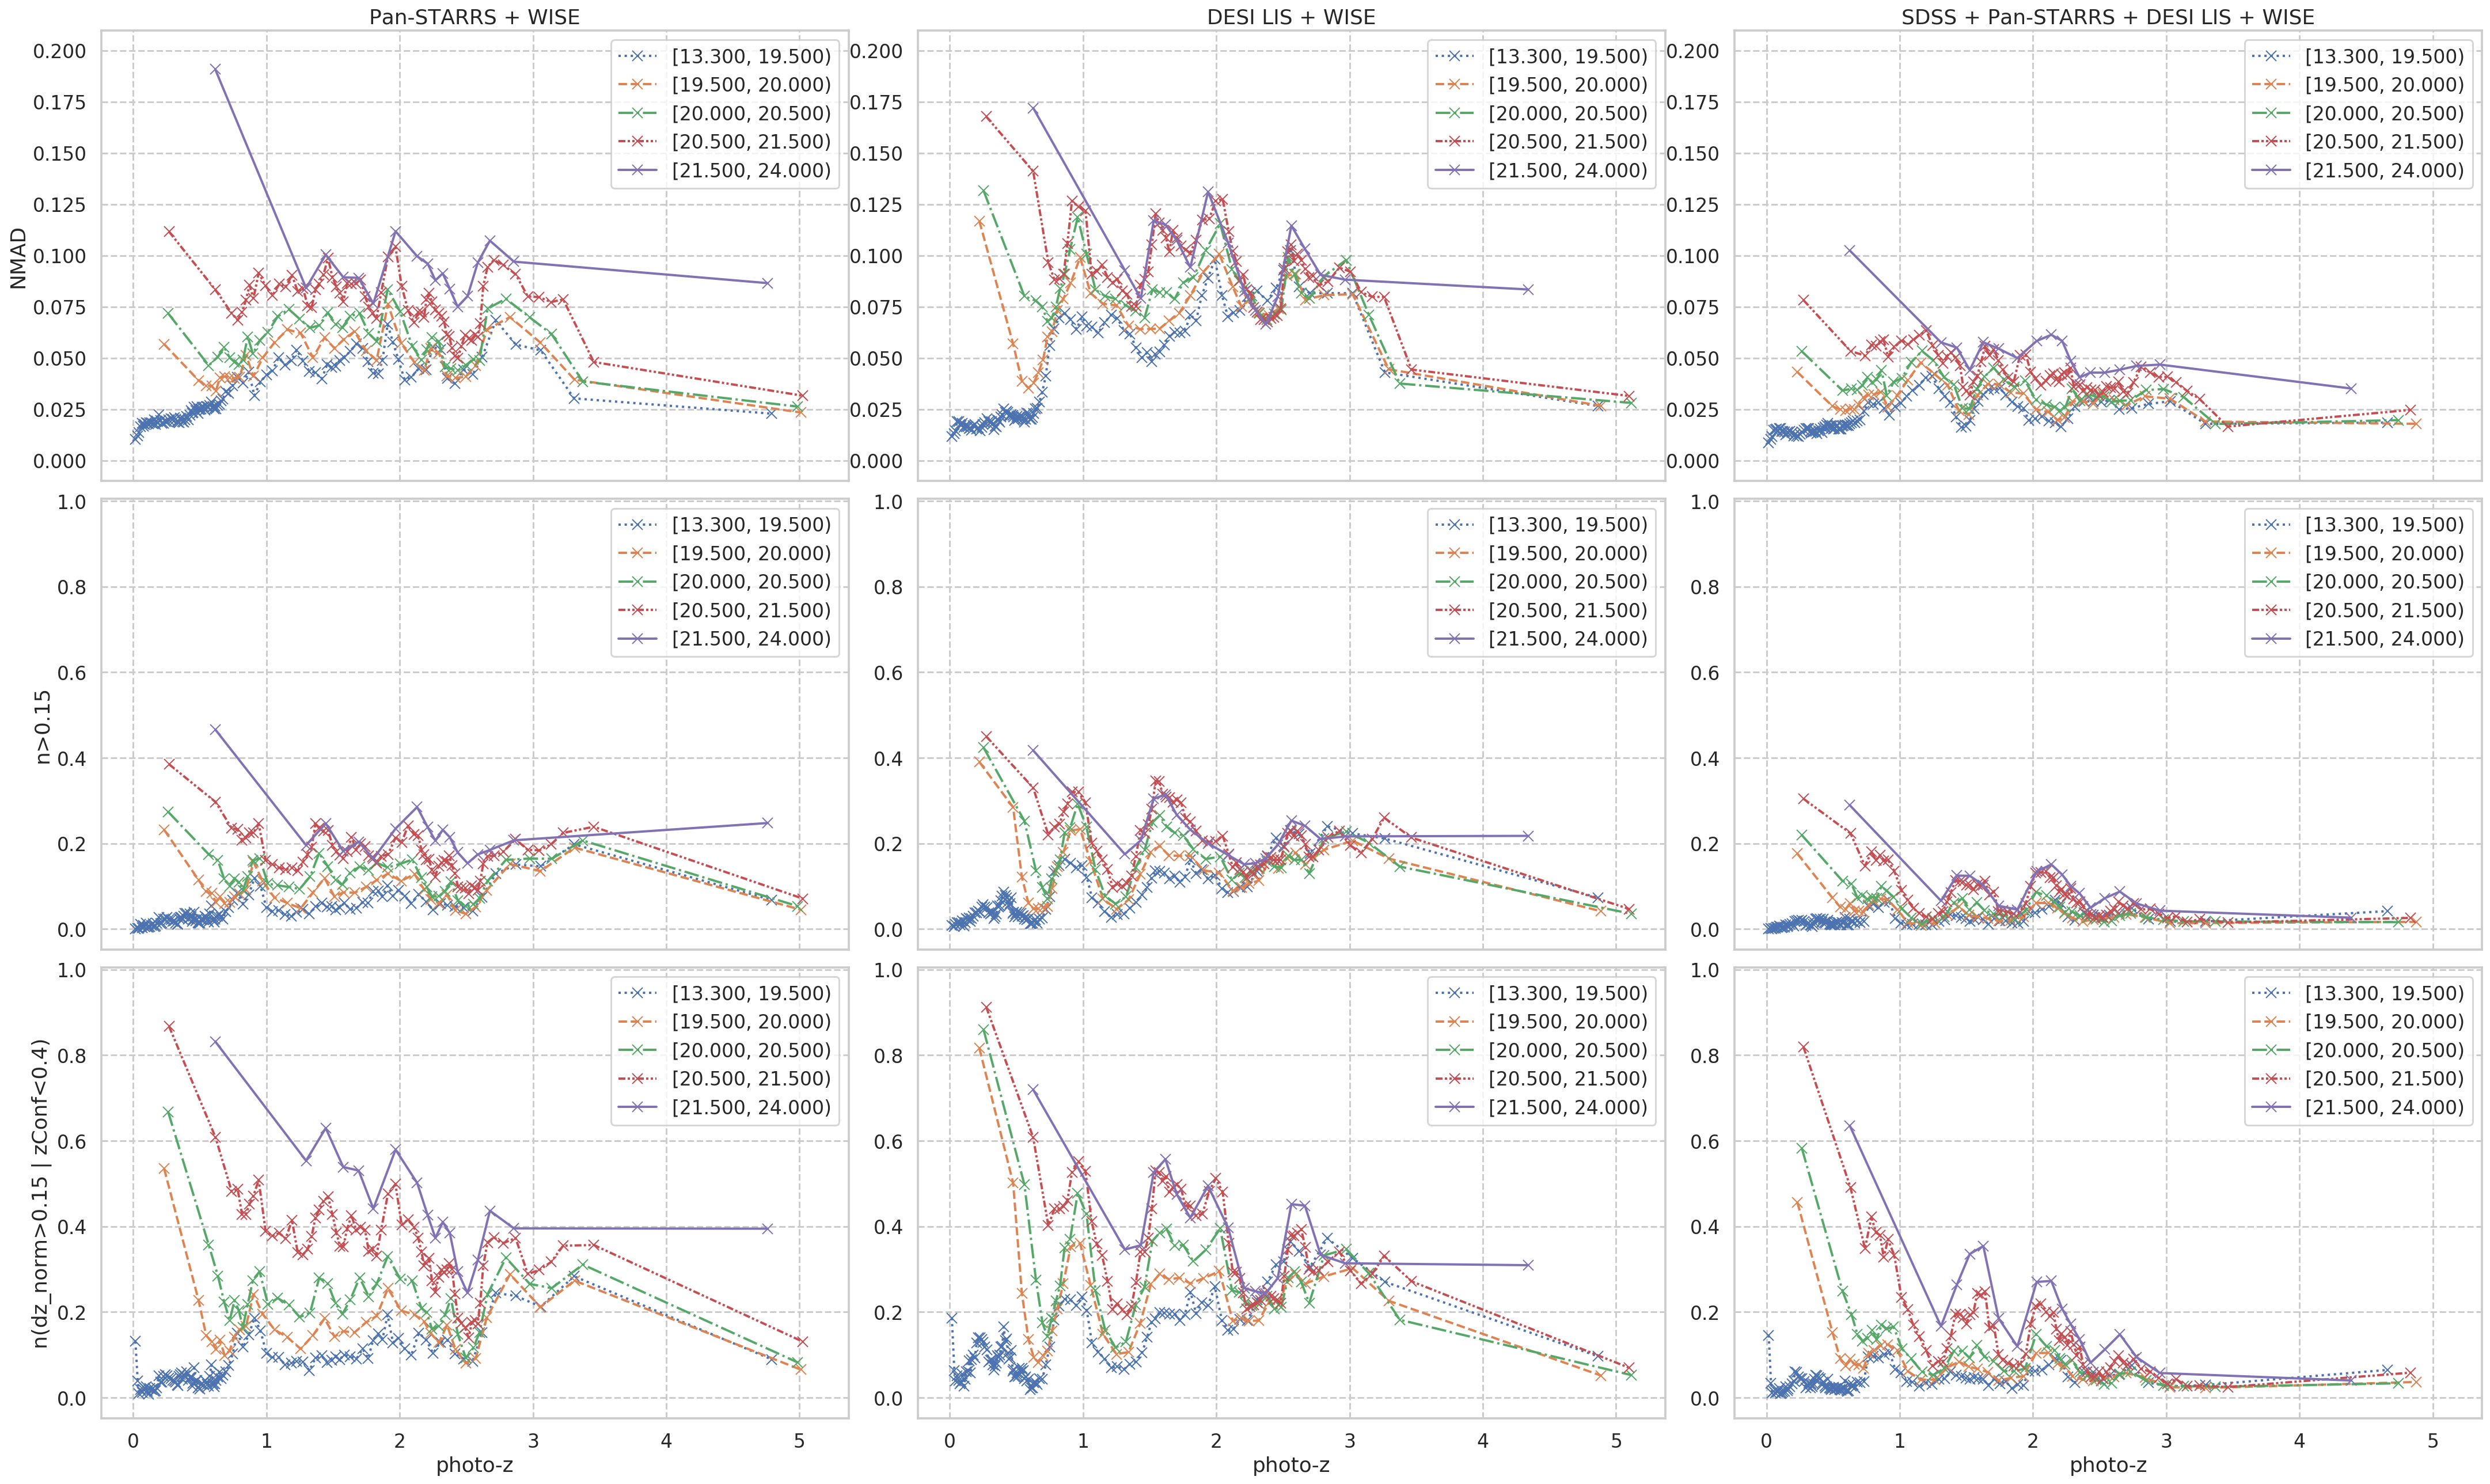
\includegraphics[width=0.9\linewidth]{images/metrics-adv-photoz-x-zmag-cv2.png}
    \caption{Метрики в зависимости от photo-z для разных порогов по $z_mag$ на кросс-валидации}
    \label{fig:my_label}
\end{figure}
\end{landscape}


\begin{landscape}
\begin{figure}
    \centering
    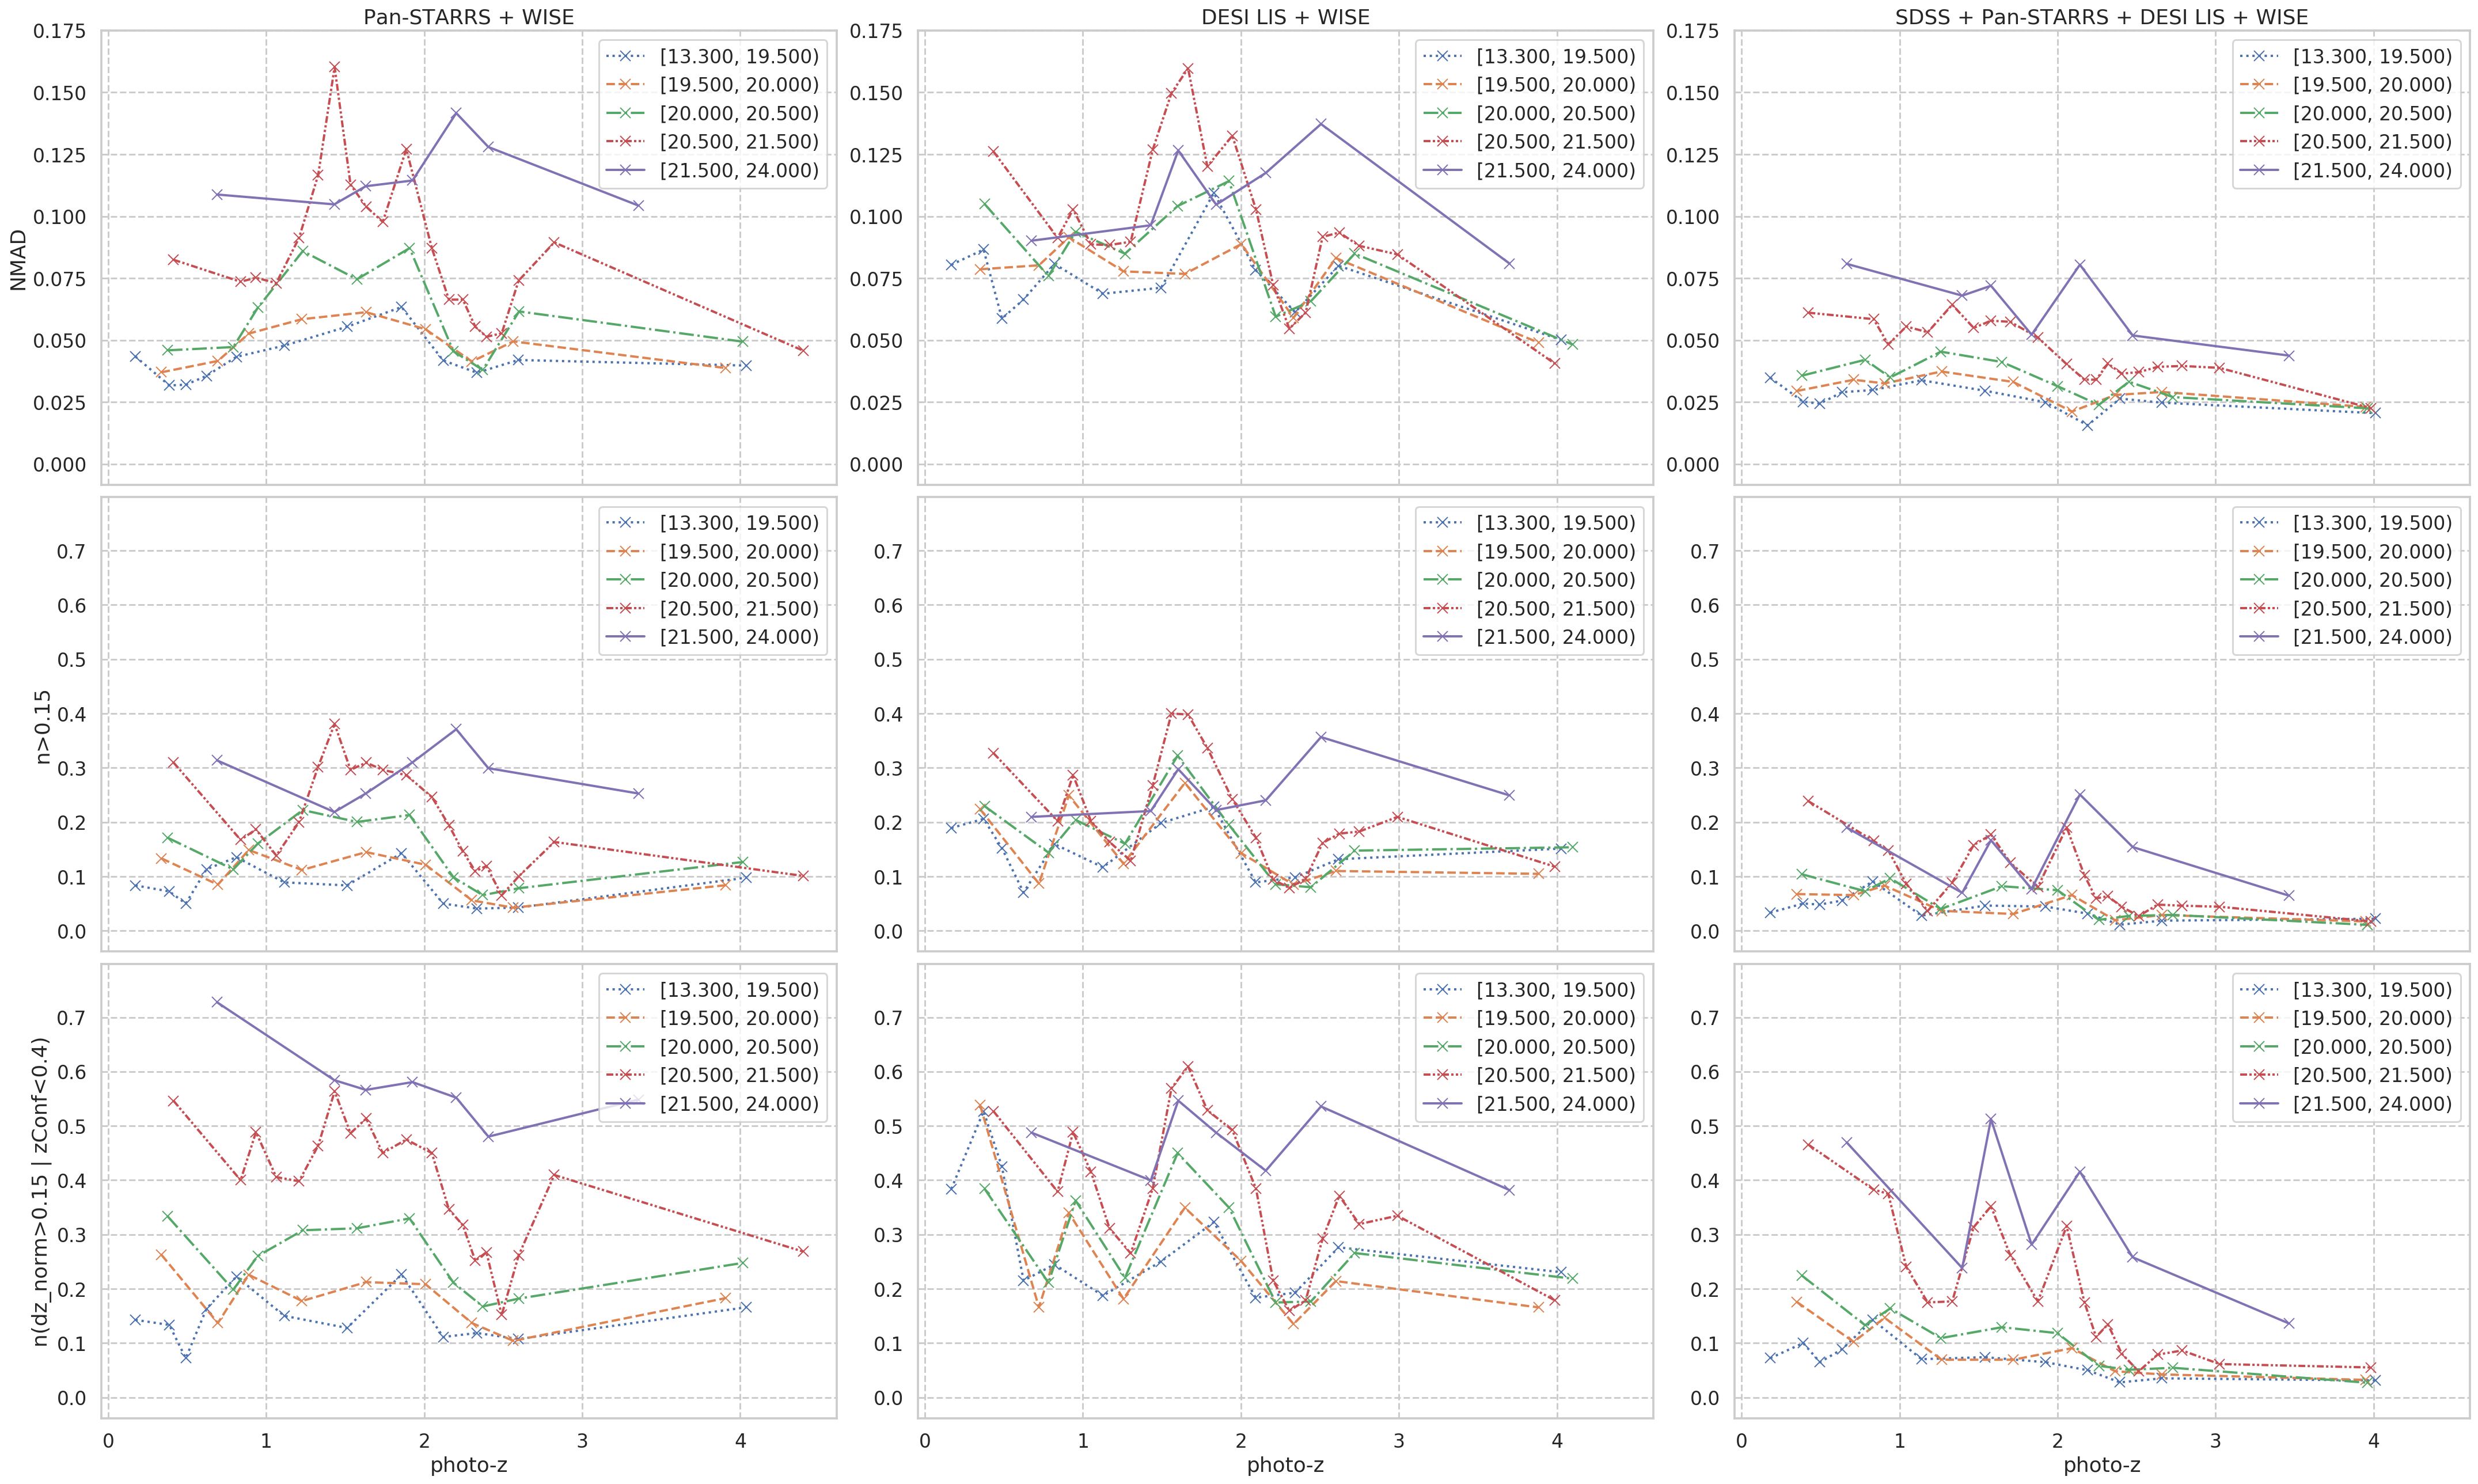
\includegraphics[width=0.9\linewidth]{images/metrics-adv-photoz-x-zmag-dr16q.png}
    \caption{Метрики в зависимости от photo-z для разных порогов по $z_mag$ на DR16q}
    \label{fig:my_label}
\end{figure}
\end{landscape}


\begin{landscape}
\begin{figure}
    \centering
    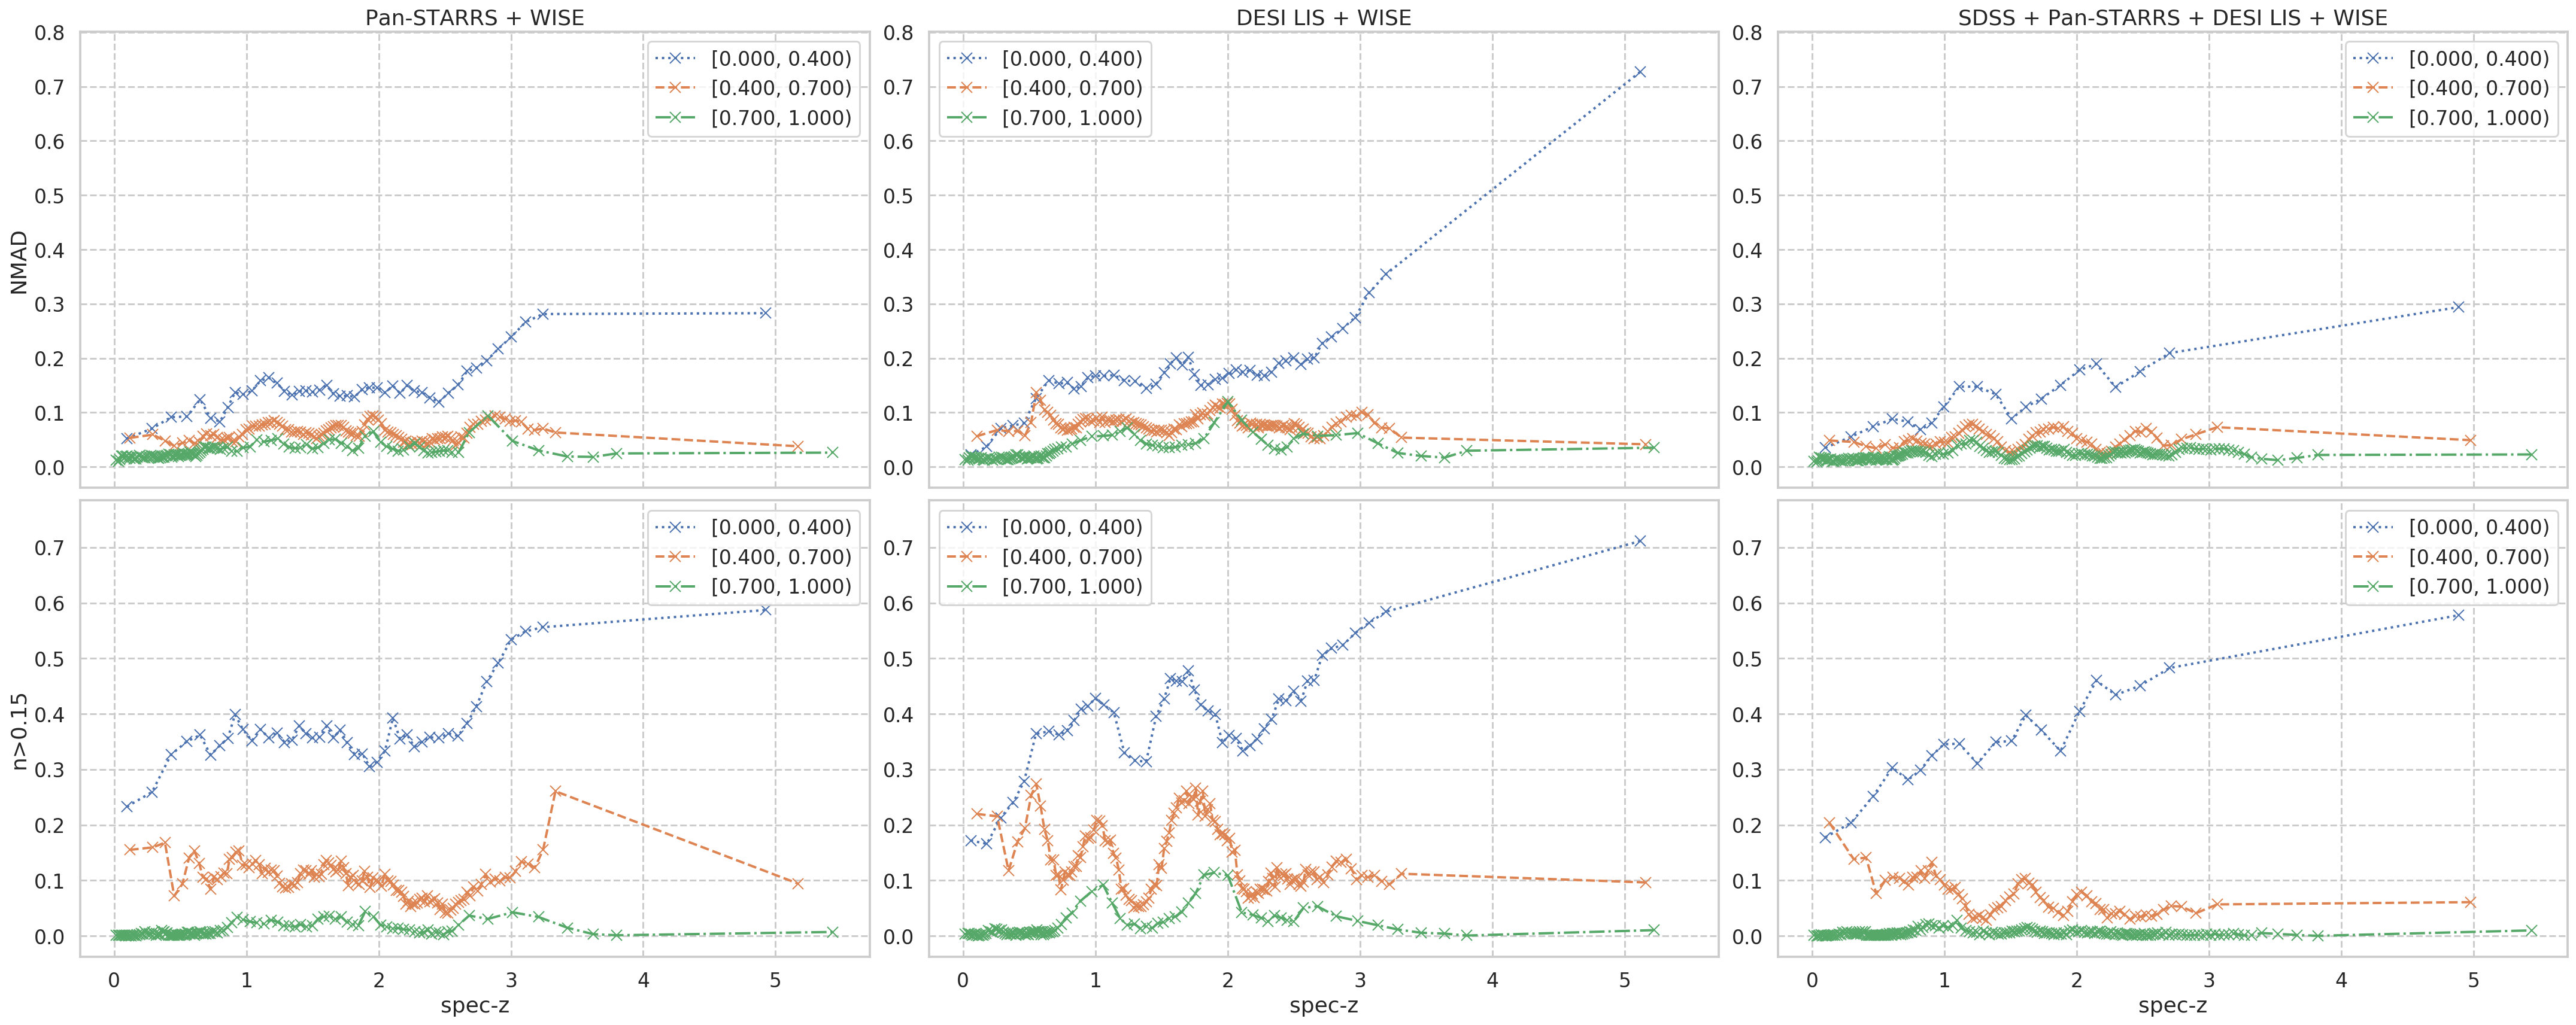
\includegraphics[width=0.9\linewidth]{images/metrics-adv-zspec-x-zconf-cv2.png}
    \caption{Метрики в зависимости от spec-z для разных порогов по zConf на кросс-валидации}
    \label{fig:my_label}
\end{figure}
\end{landscape}


\begin{landscape}
\begin{figure}
    \centering
    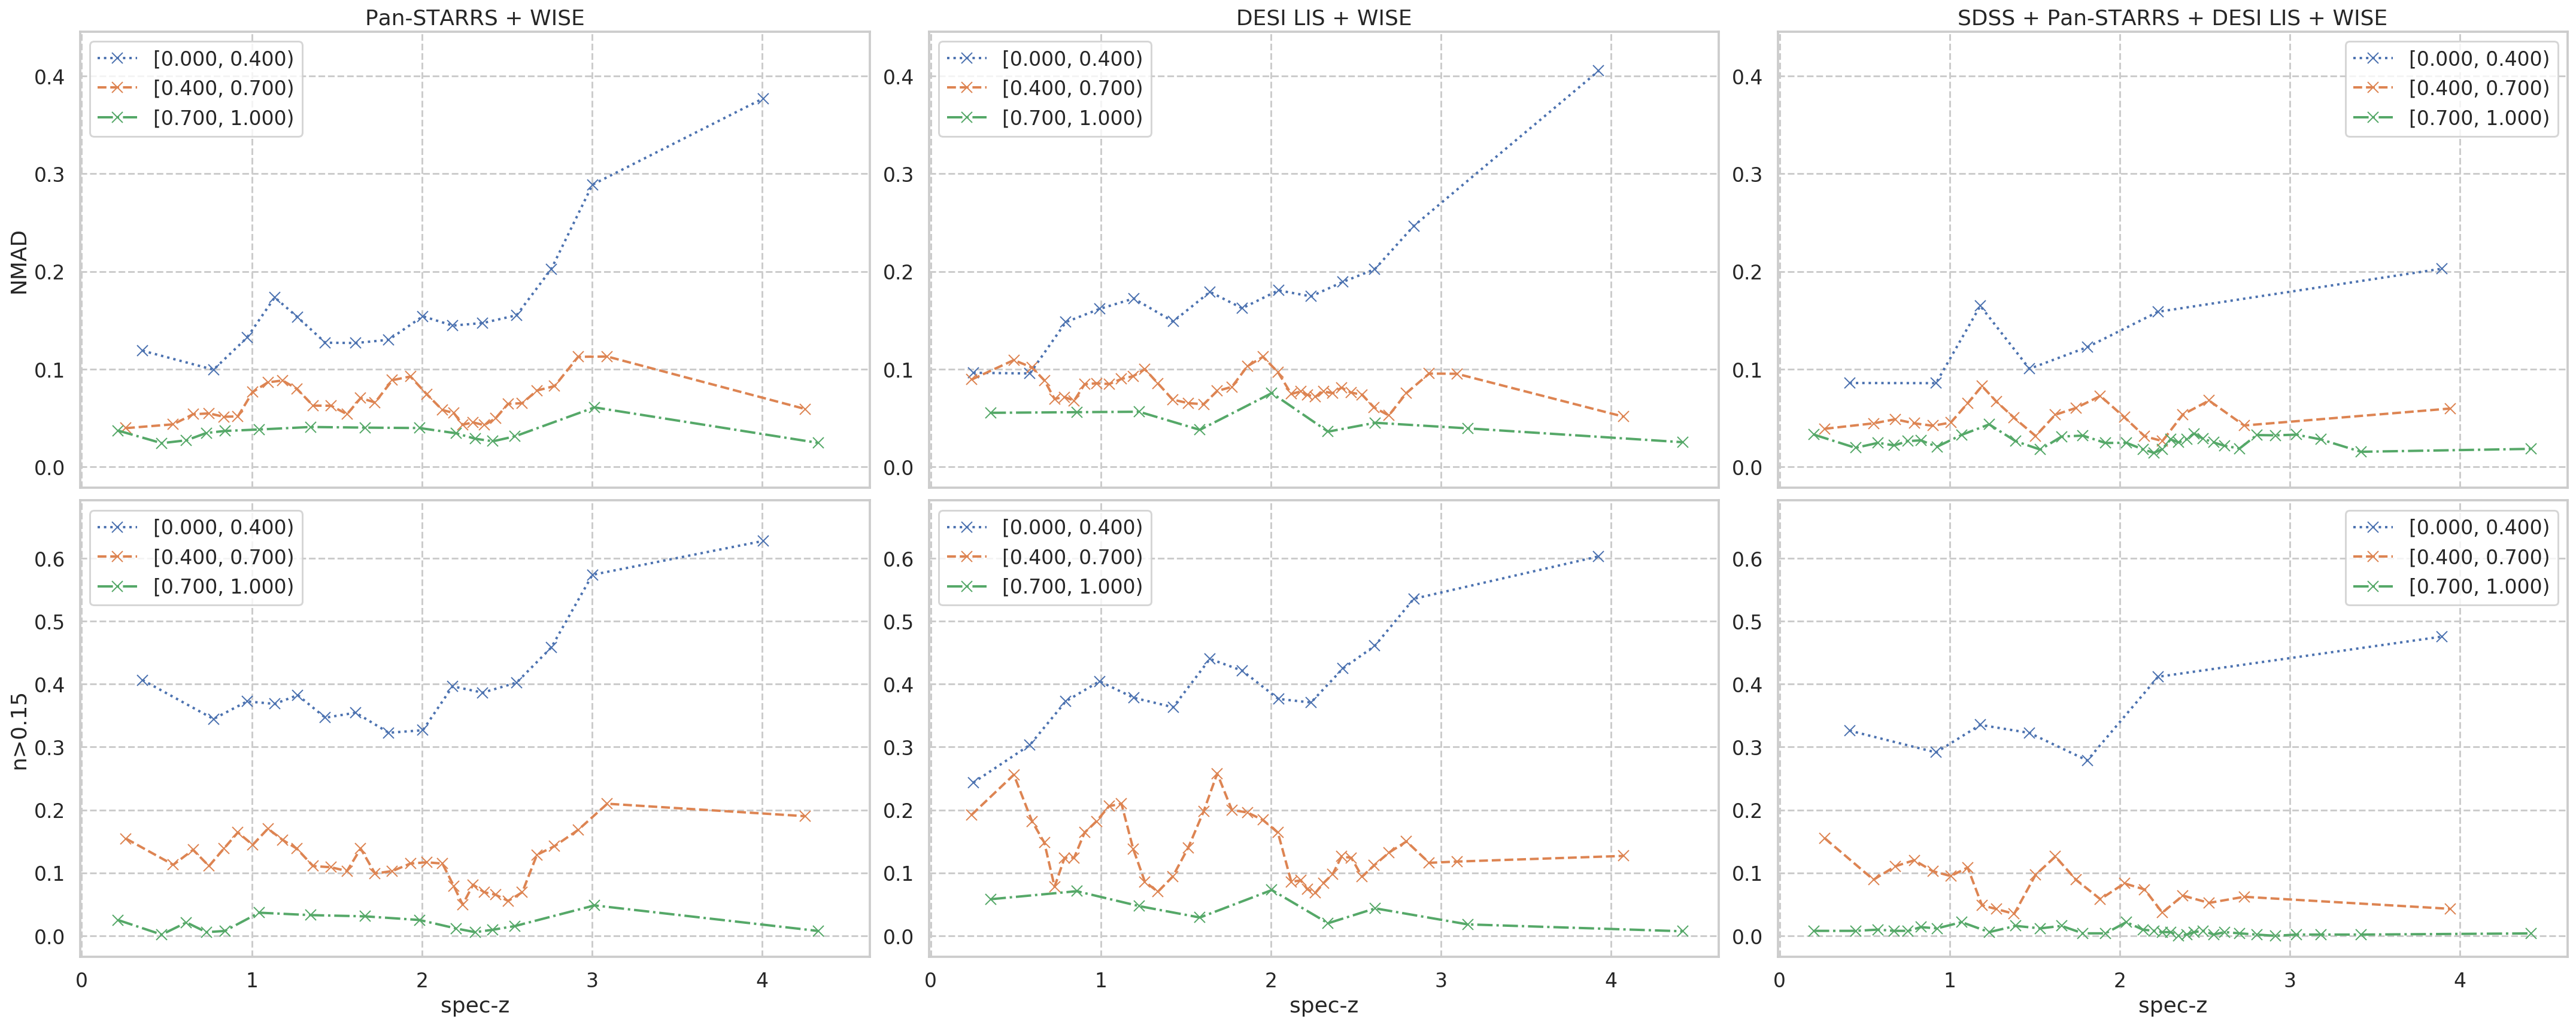
\includegraphics[width=0.9\linewidth]{images/metrics-adv-zspec-x-zconf-dr16q.png}
    \caption{Метрики в зависимости от spec-z для разных порогов по zConf на DR16q}
    \label{fig:my_label}
\end{figure}
\end{landscape}


\begin{landscape}
\begin{figure}
    \centering
    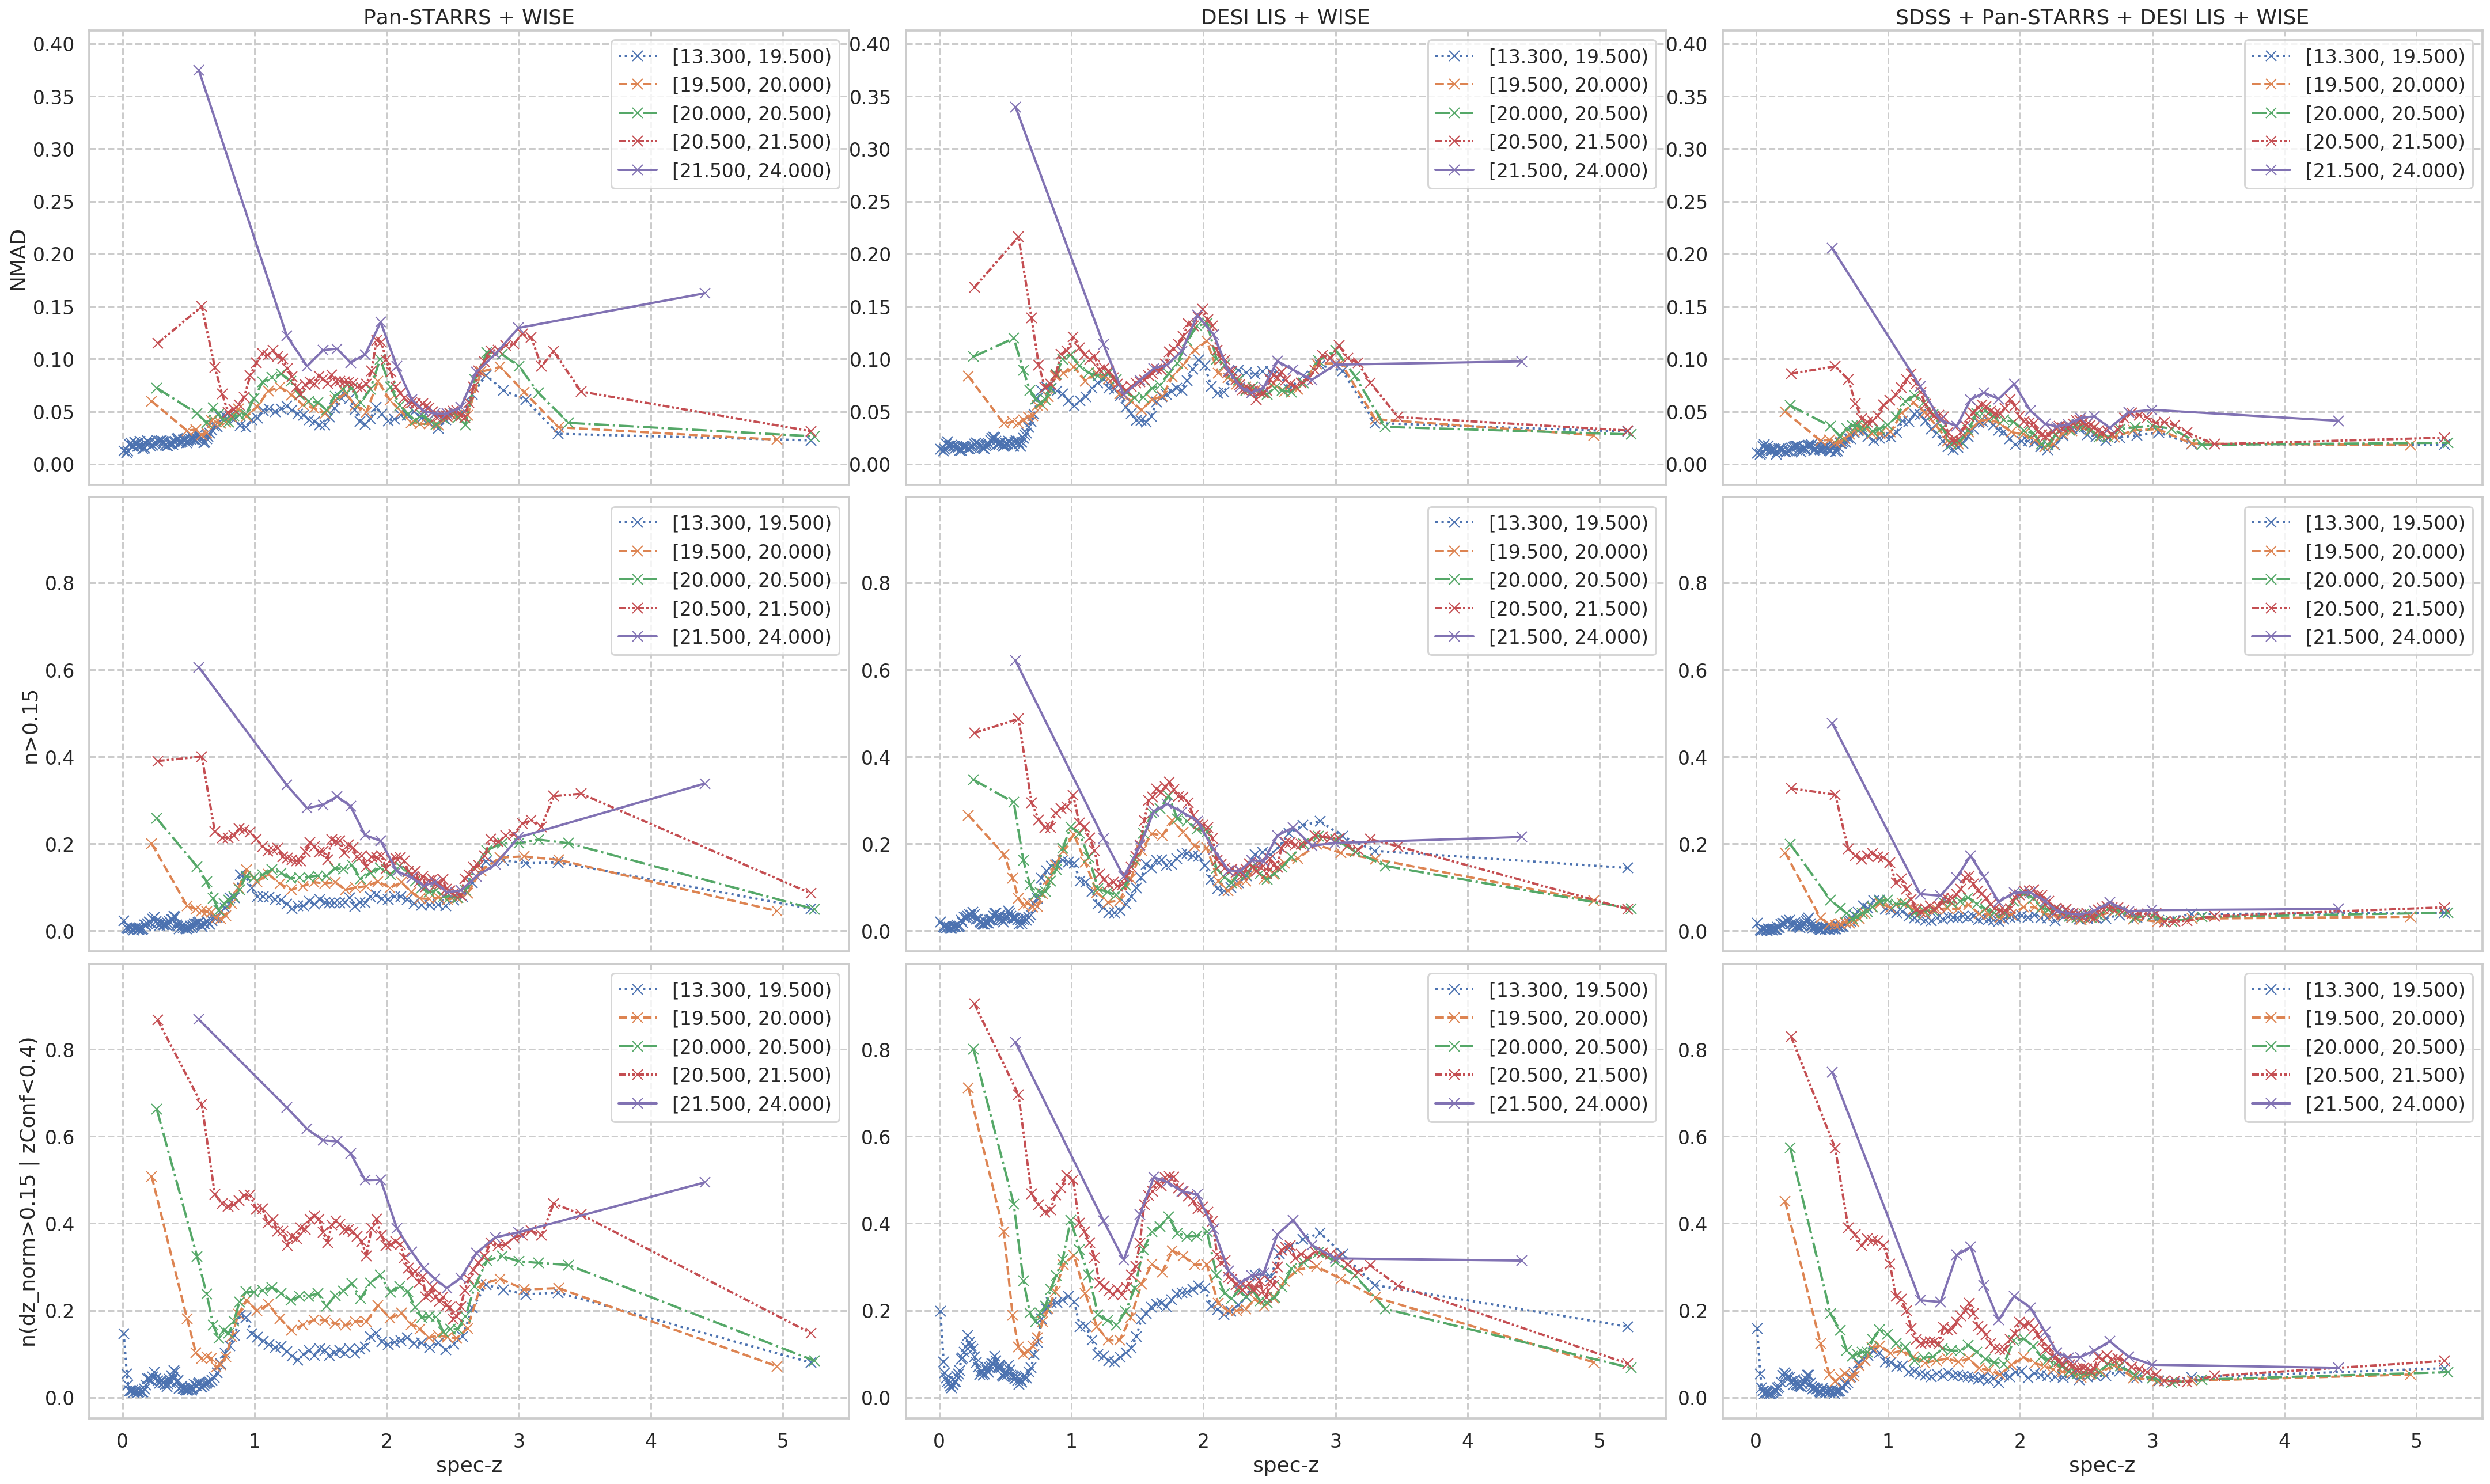
\includegraphics[width=0.9\linewidth]{images/metrics-adv-zspec-x-zmag-cv2.png}
    \caption{Метрики в зависимости от spec-z для разных порогов по $z_mag$ на кросс-валидации}
    \label{fig:my_label}
\end{figure}
\end{landscape}


\begin{landscape}
\begin{figure}
    \centering
    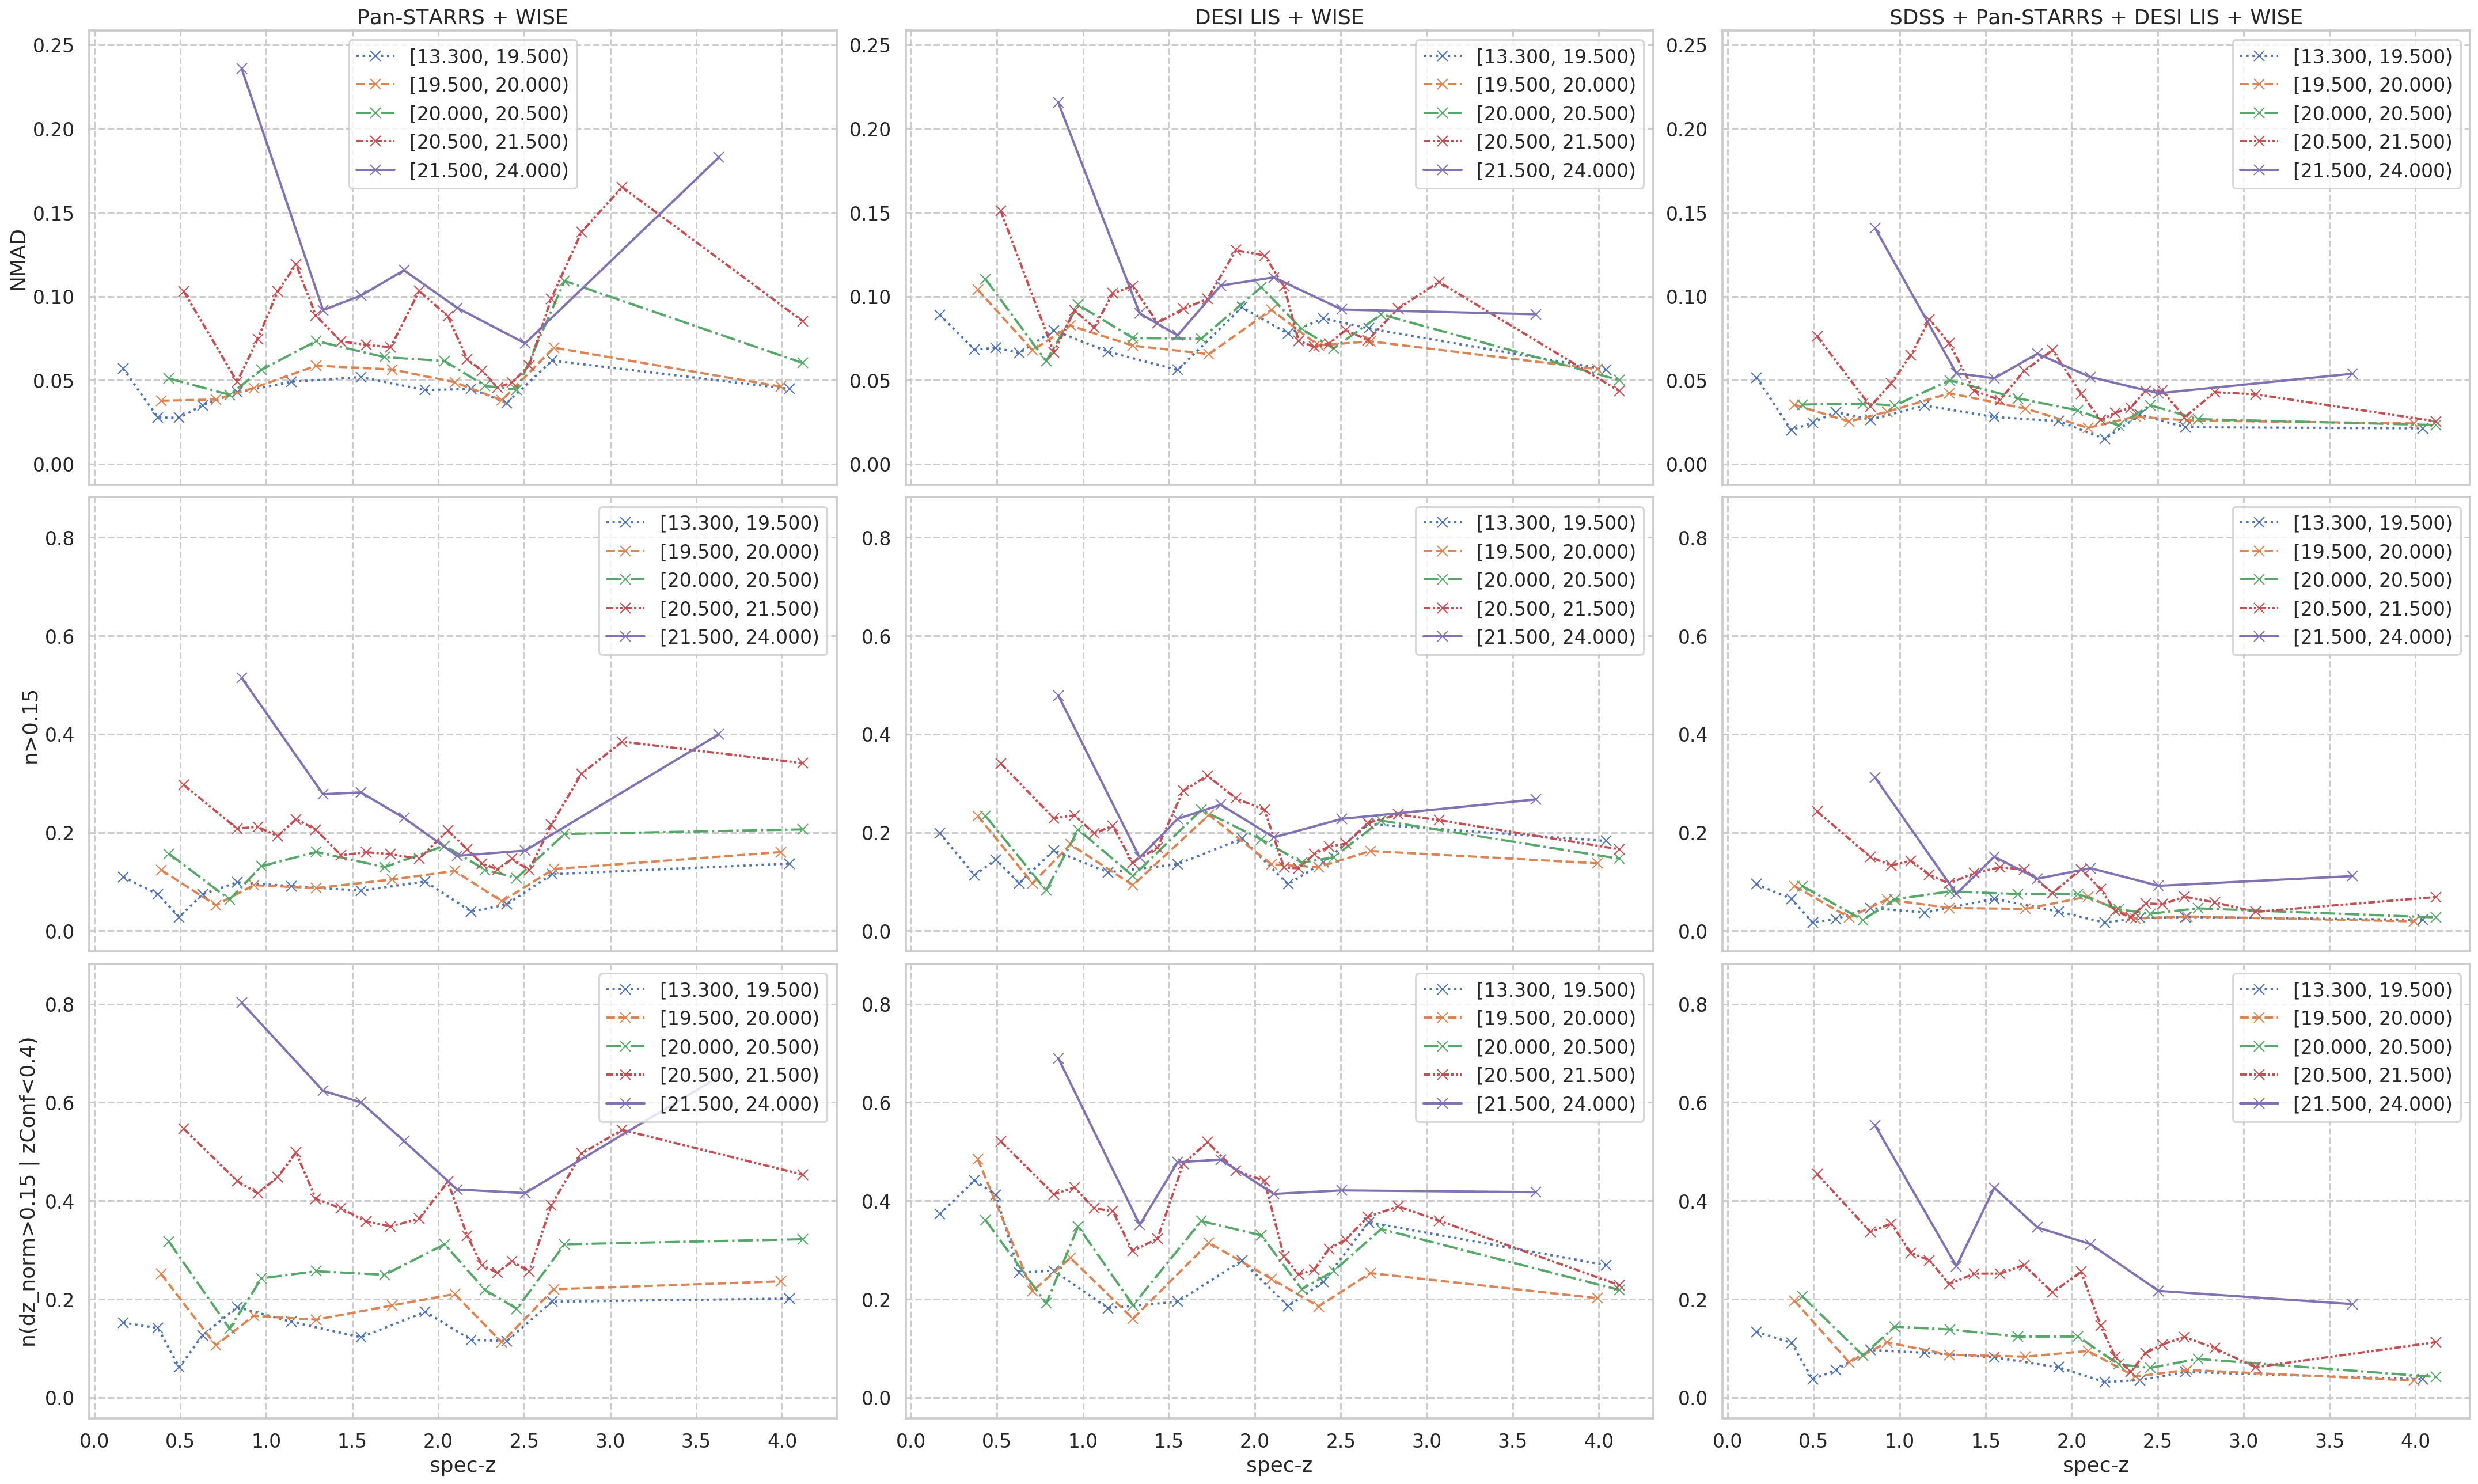
\includegraphics[width=0.9\linewidth]{images/metrics-adv-zspec-x-zmag-dr16q.png}
    \caption{Метрики в зависимости от spec-z для разных порогов по $z_mag$ на DR16q}
    \label{fig:my_label}
\end{figure}
\end{landscape}


\end{document}
